% !TeX program = xelatex
% !TeX encoding = UTF-8
\documentclass[12pt,a4paper]{article}
\usepackage{fontspec}
\usepackage[top=2.54cm,bottom=2.54cm,left=3.18cm,right=3.18cm,headheight=0pt,headsep=0pt,footskip=1.5cm]{geometry}
\setmainfont{NotoSerifSC-Regular.ttf}[Path=build-fonts/,BoldFont=NotoSerifSC-Bold.ttf]
\newfontfamily\headingfont{NotoSansSC-Regular.ttf}[Path=build-fonts/]
\newcommand{\songti}{\normalfont}
\newcommand{\heiti}{\headingfont}
\XeTeXlinebreaklocale "zh"
\XeTeXlinebreakskip=0pt plus 1pt
\usepackage{amsmath,amssymb,mathtools,bm}
\renewcommand{\theequation}{\arabic{equation}}
\usepackage{graphicx}
\usepackage{longtable,booktabs,array,tabularx,calc}
\usepackage{etoolbox}
\usepackage{float}
\usepackage{needspace}
\usepackage{caption}
\usepackage{setspace}
\usepackage{fancyhdr}
\usepackage{titlesec}
\usepackage{tocloft}
\usepackage{indentfirst}
\usepackage{enumitem}
\usepackage{fvextra}
\usepackage{xcolor}
\usepackage{xurl}
\usepackage[hidelinks]{hyperref}
\usepackage{bookmark}
\usepackage{eso-pic}
\usepackage{tikz}
\usetikzlibrary{positioning,arrows.meta,shapes.geometric,fit,backgrounds,calc}
\newcommand{\R}{\mathbb{R}}
\newcommand{\Bset}{\{0,1\}}
\DeclareMathOperator*{\argmin}{arg\,min}
\definecolor{paperGreen}{RGB}{132,168,60}
\definecolor{paperGreenDark}{RGB}{79,96,48}
\definecolor{paperGreenLight}{RGB}{212,224,192}
\definecolor{paperCream}{RGB}{245,243,232}
\tikzset{
  startstop/.style={rectangle,rounded corners=8pt,minimum width=3.2cm,minimum height=0.9cm,align=center,draw=paperGreenDark,fill=paperGreen,text=white,thick},
  process/.style={rectangle,minimum width=3.6cm,minimum height=0.9cm,align=center,draw=paperGreenDark,fill=paperCream,thick},
  decision/.style={diamond,aspect=2.1,minimum width=3.0cm,align=center,draw=paperGreenDark,fill=paperGreenLight,thick,inner sep=1pt},
  data/.style={trapezium,trapezium left angle=70,trapezium right angle=110,minimum width=3.2cm,minimum height=0.9cm,align=center,draw=paperGreenDark,fill=paperGreenLight!55,thick},
  verify/.style={rectangle,minimum width=3.4cm,minimum height=0.9cm,align=center,draw=paperGreenDark,fill=paperGreenLight,thick},
  layer/.style={rectangle,draw=paperGreenDark,dashed,inner sep=6pt},
  arrow/.style={-{Stealth[length=2.4mm]},thick,draw=paperGreenDark},
  lab/.style={font=\small,midway}
}
\newcommand{\sanhao}{\fontsize{16pt}{16pt}\selectfont}
\newcommand{\xiaosan}{\fontsize{15pt}{18.75pt}\selectfont}
\newcommand{\sihao}{\fontsize{14pt}{14pt}\selectfont}
\newcommand{\xiaosi}{\fontsize{12pt}{12pt}\selectfont}
\newcommand{\wuhao}{\fontsize{10.5pt}{10.5pt}\selectfont}
% 正文参考文献编号采用右上角标注
\newcommand{\supcite}[1]{\textsuperscript{[#1]}}

\AtBeginDocument{%
  \xiaosi\songti\setstretch{1.25}%
  % 统一所有行间公式与上下正文之间的距离
  \setlength{\abovedisplayskip}{7.5pt}%
  \setlength{\belowdisplayskip}{7.5pt}%
  \setlength{\abovedisplayshortskip}{7.5pt}%
  \setlength{\belowdisplayshortskip}{7.5pt}%
}
\setstretch{1.25}
\setlength{\parindent}{2em}
\setlength{\parskip}{7.5pt}
\pagestyle{fancy}
\fancyhf{}
\fancyfoot[C]{\xiaosi\thepage}
\renewcommand{\headrulewidth}{0pt}
\renewcommand{\footrulewidth}{0pt}
\fancypagestyle{plain}{\fancyhf{}\fancyfoot[C]{\xiaosi\thepage}\renewcommand{\headrulewidth}{0pt}\renewcommand{\footrulewidth}{0pt}}
\newcommand{\ChineseNumber}[1]{%
  \ifcase#1 零\or 一\or 二\or 三\or 四\or 五\or 六\or 七\or 八\or 九\or 十%
  \or 十一\or 十二\or 十三\or 十四\or 十五\or 十六\or 十七\or 十八\or 十九\or 二十\else #1\fi}
\renewcommand{\thesection}{\ChineseNumber{\value{section}}、}
\renewcommand{\thesubsection}{（\ChineseNumber{\value{subsection}}）}
\renewcommand{\thesubsubsection}{（\arabic{subsubsection}）}
\renewcommand{\theparagraph}{（\arabic{paragraph}）}
\renewcommand{\thesubparagraph}{\arabic{subparagraph}）}
\titleformat{\section}{\centering\heiti\xiaosan}{\thesection}{0.5em}{}
\titlespacing*{\section}{0pt}{12pt}{6pt}
\titleformat{\subsection}{\raggedright\heiti\sihao}{\thesubsection}{0.5em}{}
\titlespacing*{\subsection}{0pt}{6pt}{0pt}
\titleformat{\subsubsection}{\raggedright\songti\xiaosi\bfseries}{\thesubsubsection}{0.5em}{}
\titlespacing*{\subsubsection}{0pt}{6pt}{0pt}
\titleformat{\paragraph}[runin]{\raggedright\songti\xiaosi}{\theparagraph}{0.5em}{}
\titleformat{\subparagraph}[runin]{\raggedright\songti\xiaosi}{\thesubparagraph}{0.5em}{}
\setcounter{secnumdepth}{5}
\setcounter{tocdepth}{3}
% 目录按标题层级逐级缩进：一级顶格，二级和三级依次右移
\cftsetindents{section}{0em}{4em}
\cftsetindents{subsection}{0em}{4em}
\cftsetindents{subsubsection}{0em}{4em}
\makeatletter
\let\paper@l@subsection\l@subsection
\let\paper@l@subsubsection\l@subsubsection
\renewcommand*{\l@subsection}[2]{\paper@l@subsection{\hspace*{2em}#1}{#2}}
\renewcommand*{\l@subsubsection}[2]{\paper@l@subsubsection{\hspace*{4em}#1}{#2}}
\makeatother
\renewcommand{\figurename}{图}
\renewcommand{\tablename}{表}
\DeclareCaptionFont{captioncn}{\songti\xiaosi\setstretch{1.0}}
\DeclareCaptionLabelSeparator{twospaces}{\hspace{2em}}
\captionsetup{font=captioncn,labelsep=twospaces,justification=centering,singlelinecheck=true}
\captionsetup[table]{position=top}
\captionsetup[figure]{position=bottom}
\renewcommand{\thefootnote}{\textcircled{\scriptsize\arabic{footnote}}}
\graphicspath{{media/}}
\makeatletter
\def\maxwidth{\ifdim\Gin@nat@width>\linewidth\linewidth\else\Gin@nat@width\fi}
\def\maxheight{\ifdim\Gin@nat@height>0.82\textheight 0.82\textheight\else\Gin@nat@height\fi}
\def\fps@figure{htbp}
\patchcmd\longtable{\par}{\if@noskipsec\mbox{}\fi\par}{}{}
\makeatother
\AtBeginEnvironment{tabular}{\songti\xiaosi\setstretch{1.0}}
\AtBeginEnvironment{longtable}{\songti\xiaosi\setstretch{1.0}}
\setkeys{Gin}{width=\maxwidth,height=\maxheight,keepaspectratio}
\setlength{\emergencystretch}{3em}
\providecommand{\tightlist}{\setlength{\itemsep}{0pt}\setlength{\parskip}{0pt}}
\urlstyle{same}
\hypersetup{pdfauthor={},pdftitle={暖城向新·热力不息}}

\newcommand{\EnableBodyBackground}{%
  \AddToShipoutPictureBG{%
    \AtPageLowerLeft{%
      
\includegraphics[width=\paperwidth,height=\paperheight]{body-background.jpg}%
    }%
  }%
}

\newenvironment{refsectionflush}
  {\par\sloppy\setlength{\parindent}{0pt}\setlength{\parskip}{0pt}}
  {\par\fussy}
\newcommand{\refentry}[2]{%
  \par\noindent\hangindent=2em\hangafter=1
  [#1]\enspace #2\par}

\begin{document}

\AddToShipoutPictureBG*{%
  \AtPageLowerLeft{
\includegraphics[width=\paperwidth,height=\paperheight]{cover.jpg}}%
}
\thispagestyle{empty}
\null
\clearpage
\EnableBodyBackground
\pagestyle{empty}
\begin{center}
{\songti\sanhao\bfseries\setstretch{1.0} 暖城向新·热力不息\par}
\vspace{18pt}
{\heiti\sihao 摘\quad 要\par}
\end{center}
\vspace{3pt}
\par\indent 针对我国不同地区供热基础、气候条件和资源禀赋差异显著，传统规划方法难以同时协调存量资产利用、清洁能源消纳、管网温位、建筑舒适和极端天气保供等问题，本文研究既有大型集中供热系统低碳化重构、分散式独立供热系统清洁化转型以及夏热冬冷地区高品质供热系统新建三类典型场景。围绕“建什么、建多大、何时建设或退役、不同工况下怎样运行”，建立兼顾经济性、低碳性、可靠性与工程可实施性的城镇供热源荷匹配与规划寻优模型。

模型采用\textbf{“公用模型内核+场景适配器”}的总体结构。公用内核以多阶段资产演化为主线，将热源、管网、储热、建筑、电力系统、碳排放和风险因素纳入同一决策体系；以带温位的节点能量守恒描述不同品位热能的供需匹配，以容量、可用率、启停和爬坡约束描述设备运行，以储热递推和建筑热状态方程反映跨时段耦合，并统一核算投资、运行、维护、残值、能源费用和碳成本。模型以\textbf{生命周期净成本}为基础目标，将碳排放、化石峰值依赖、室内舒适、配电接入、施工能力和安全保供作为目标边界或约束，避免以单一成本指标掩盖供热不足、温位不匹配和工程不可行。

三类场景通过专用模块体现差异。三个场景共用同一条求解管线：先在代表时段上完成投资---运行联合规划，再冻结投资方案进行完整时序运行校核，规划阶段与回放阶段分别报告求解状态与间隙。乌鲁木齐在此基础上协调化石热源退役、工业余热与大型热泵接入、网络降温、末端改造和储热配置；固原重点考察设施选址、用户分配、燃料库存、配电与孤岛保供；武汉重点比较不同供热形态及其配电边界。热湿、噪声、地源多年平衡等未在本次算例中验证的功能，仅作为可选扩展说明。

计算过程按照\textbf{“数据审计---候选链预筛---模型装配---规划求解---压力测试---工程校核”}组织。统一各类输入的单位、时间尺度与来源，剔除受源温、距离、场地、配电和法规限制的不可行候选；固定投资变量后，重调度寒潮、余热下降、价格变化、需求响应退出和关键故障情景。三个场景的模拟窗口分别为4392 h、4392 h和2880 h，各给出代表时段规划解与冻结投资后的全季运行解，两类解分别报告求解状态与间隙。补充验证对三个场景各执行一次2023日日历年8760 h连续回放，规划层与回放层均取得状态0解、失供率为0，并分别通过15、16、17项验收条目。结果可为供热方案比选、投资安排与极端保供提供可追溯的决策依据。

\vspace{-4.5pt}
\noindent{\heiti\xiaosi 关键词：}{\songti\xiaosi 城镇供热；源荷匹配；规划寻优；低碳转型；供热可靠性}
\clearpage
\thispagestyle{empty}
\begin{center}{\heiti\sihao 目\quad 录}\end{center}
\begingroup
\setlength{\parskip}{0pt}
\setlength{\cftbeforesecskip}{1pt}
\makeatletter
\@starttoc{toc}
\makeatother
\endgroup
\clearpage
\pagenumbering{arabic}
\setcounter{page}{1}
\pagestyle{fancy}
\section{研究背景与文献综述}

\subsection{城镇供热转型背景}

城镇供热兼具公共服务和能源消费属性，涉及热源、管网、换热站、建筑末端、电力系统及用户行为等多个环节。热能消费约占全球终端能源消费的一半，可再生热力的增长仍不足以支撑供热部门快速脱碳\supcite{26}。我国相关政策也对建筑用能电气化、可再生能源替代和既有建筑节能改造提出了明确要求\supcite{24}，供热规划因而需要由单一热源扩容转向源、网、荷、储协同配置。

我国各地区的气候、资源和既有资产差异显著。北方大型城市侧重既有热网与热源的改造和退出，县城及农村地区需要确定集中与分散供热边界，夏热冬冷地区还需统筹冬季供热、夏季供冷、生活热水与配电容量。不同场景不能沿用同一技术组合，需要建立可按场景配置的规划方法。

\subsection{建筑热环境与居民用热需求}

老旧建筑保温不足、空气渗透、末端老化和二次网失调会造成近端过热、远端欠热、回水温度偏高及泵耗增加。图\ref{fig:building-heating-imbalance}直观展示了围护结构散热、管网输配和房间温度不均之间的关系。既有建筑节能水平差异较大\supcite{25}，仅改造热源并不能保证室温和用热公平同步改善。因此，规划中还应考虑围护结构、散热末端、热计量、控制条件和最不利房间。

\begin{figure}[H]
\centering
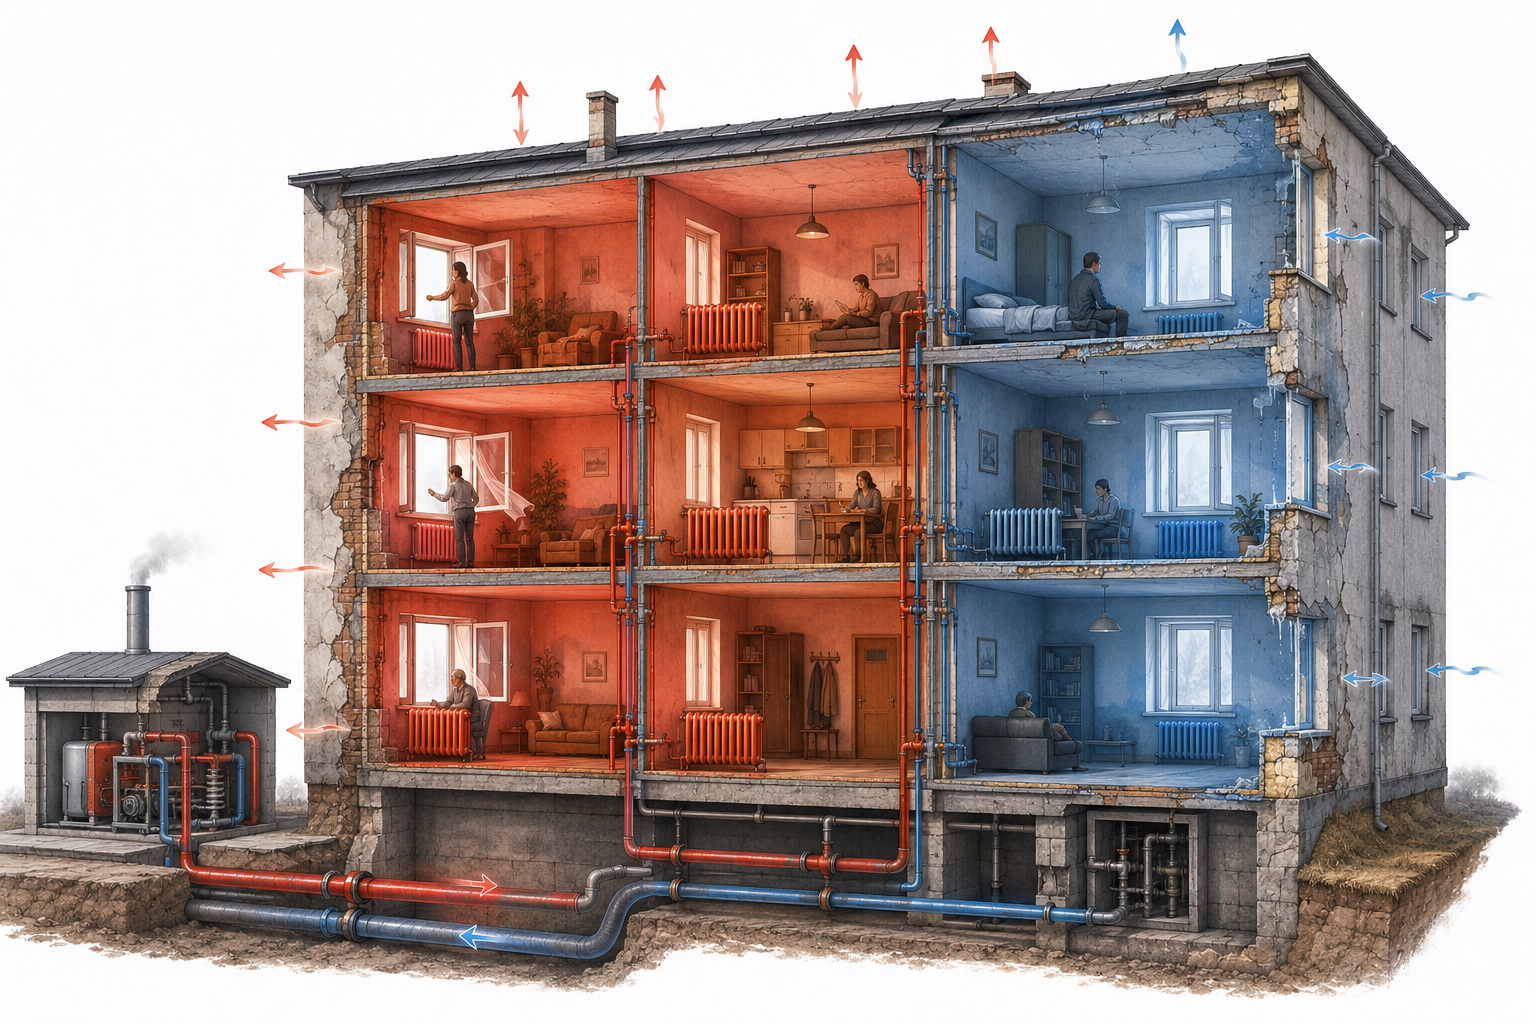
\includegraphics[width=0.75\textwidth,height=0.32\textheight,keepaspectratio]{media/building_heating_imbalance.png}
\caption{老旧建筑供热不均与热损失示意图}
\label{fig:building-heating-imbalance}
\end{figure}

热泵等电气化设备可能抬升冬季电力峰值，围护结构和末端改造又会增加初始投资。方案评价除成本和碳排放外，还需兼顾舒适度、配电容量、居民可负担性、维护条件和极端保供能力。

\subsection{传统供热规划的局限}

传统方法多采用“先定技术路线、再核算容量、最后用典型日校核”的流程，难以反映热源、管网、建筑、储热和电网之间的耦合关系。例如，管网降温会影响末端改造，热泵扩容会增加配电投资，储热替代峰值容量还受到充放热功率和时序状态约束。

室外温度、资源可用率、能源价格和设备故障均具有时变性。仅依据年平均负荷或单个设计日规划，难以同时保证全年经济性和寒潮期间的供热可靠性。因此，需要联合确定设备建设、改造、退役与逐时运行方式。

\subsection{国内外研究进展}

\subsubsection{国内研究进展}

国内供热低碳转型主要包括三类路径：既有集中供热系统的热源与管网改造，县城及农村地区的分散清洁供热，以及建筑节能与智慧供热改造。相关实践已覆盖工业余热、大型热泵、低温热网、生物质、太阳能、热计量和气候补偿控制等技术，但各类项目多围绕单项设备或局部系统展开。建筑改造后热源和管网容量如何调整、不同地区集中与分散供热边界如何确定、需求响应能够提供多少稳定调节能力，仍需统一量化。

国内研究已采用综合能源系统优化、多目标规划、鲁棒优化和需求响应等方法，但对最不利房间、二次网失调、回水温度、居民可负担性以及极端工况可靠性的处理仍不充分，跨场景模型结构也较少。

\subsubsection{国外研究进展}

欧洲已形成建筑节能、区域供热、热泵、余热利用和低温热网相结合的技术路径。2024年空间供暖和生活热水约占欧盟家庭终端能源消费的77.1\%\supcite{27}。北欧地区通过地方热力规划确定区域供热与个体供热的服务边界，并将低温输配、余热、大型热泵、可再生能源和季节储热协同配置；第四代区域供热研究进一步强调需求侧柔性与低温热源利用\supcite{20,21}。

国外研究已由单设备优化转向综合规划，常用混合整数规划、多目标优化、随机或鲁棒优化等方法分析热源容量、网络拓扑、储热和建筑柔性。但研究结论受资源、市场和监管条件影响较大，部分模型仍聚焦单一环节，对大规模热泵带来的配电峰值及跨系统约束考虑不足。

相关研究主要围绕可再生能源、电力、储能、分布式发电、数学优化和碳中和等主题展开，余热、可再生热、热储能与微电网之间具有较强关联。供热转型研究已由单一热源技术评价逐步转向能源系统协同与优化决策。

\subsubsection{研究不足与本文切入点}

综合国内外研究，现有成果已经形成较丰富的技术库，但从单项技术可行性走向区域转型方案，仍存在以下不足。

第一，系统边界较为分散。热源、管网、建筑、储热和配电系统常由不同模型分别处理，导致热源侧的清洁替代无法同步反映末端适配、回水温度、配电增容和建筑改造需求。热量在总量上平衡，并不意味着温位、空间位置和输配能力同时满足要求。

第二，规划与运行衔接不足。部分研究使用年平均量或少量典型日确定容量，对设备建设、改造和退役的年度时序描述较弱；另一些研究侧重逐时调度，却将容量和网络结构视为已知条件。由此得到的方案可能具有较好的年平均指标，但在寒潮、资源中断或设备故障时缺少可靠容量。

第三，低碳、经济与民生目标缺少统一权衡。年度清洁热占比不能直接代表极寒峰值的化石依赖程度，最低成本方案也未必满足最不利房间温度、居民可负担性和关键建筑保供要求。若不区分生命周期成本、运行现金成本和风险成本，方案之间也难以公平比较。

第四，物理精度与求解规模之间存在矛盾。连续水力、温度衰减、建筑热惯性和设备性能曲线能够提高工程真实性，但全部直接纳入大规模整数模型会显著增加计算难度；过度简化又可能产生温位不匹配、储热状态不闭合或网络输送不可行的方案。现有研究对优化模型与工程校核如何分工，尚缺少统一、可复核的流程。

第五，模型的场景迁移能力有限。既有大型热网重构、分散供热清洁化和夏热冬冷地区新建系统在资产基础、负荷特征和主导约束上差异明显，分别建模虽能体现局部特点，却难以形成一致的数据清单、指标定义和比较方法。

基于上述不足，本文以“公用模型内核+场景适配器”为总体结构，将资产演化、带温位能量平衡、储热、建筑状态、电力约束、成本碳排和可靠性纳入统一框架，并针对三类场景加载差异化约束。规划模型负责筛选建设、改造、退役和运行组合，寒潮、资源中断、设备故障及价格变化等情景用于压力测试；本次完成节点热平衡、容量、储热和关键断面的数值校核，连续水力与房间级温度作为工程扩展，从而形成可计算、可比较的供热转型决策流程。


\subsection{数学建模的决策支撑}

供热转型已经由单一设备选型发展为跨年度、跨区域、跨能源载体并包含不确定性的系统组合决策。热源退役、工业余热接入、管网降温、建筑改造、储热配置和配电增容之间相互影响，任何一项决策都不能脱离其他环节单独评价。传统经验和单项仿真能够判断某一设备或既定方案是否可行，但难以在大量候选组合中同时比较建设时序、容量配置、运行方式和极端工况下的可靠性。

数学模型将热量守恒、温位兼容、设备容量、建筑舒适、储热状态、电网接入和可靠性要求转化为统一的变量与约束，并在工程边界满足的条件下比较生命周期成本、碳排放和风险。模型采用统一的度量方式描述热源、管网、建筑和电网之间的关系，用于筛选满足约束的候选路径。

本文采用“优化筛选---压力测试---数值校核”的计算流程。首先检查负荷、气象、设备性能、能源价格和碳排放因子的来源与适用范围；其次核验热量、电力、储热和等效热状态的守恒残差，并在寒潮、余热下降、设备故障和电网受限等情景下重新调度；最后检查最大流量管段、最远换热站和回水异常节点。连续水力、房间级温度以及校核结果自动回写属于扩展功能，本次未启用。

模型可用于候选技术组合筛选、热源与储热容量配置、管网改造与降温路径、建筑改造顺序、设备建设和退役时序以及极端工况下的风险识别。数学建模负责规划决策和方案比较，工程专业仍负责资源调查、设备选型、施工图设计、地质勘察、环保与配电审批及现场调试。只有模型约束、压力测试和专业工程校核均通过的方案，才能作为实施依据。


\clearpage
\section{负荷预测与协同优化模型}

\subsection{基本假设}

为明确模型适用范围，作如下假设：
\begingroup
\setlength{\parskip}{0pt}
\newcommand{\assumptionline}[2]{\par\noindent\hangindent=1.8em\hangafter=1 #1.\hspace{0.5em}#2}
\assumptionline{1}{研究区域由热源节点、管网节点、换热站和典型建筑构成，同类建筑在保持负荷特征的前提下聚合处理；}
\assumptionline{2}{气象、建筑参数、设备性能和能源价格按1~h时间步长输入；时间区间采用左闭右开形式，乌鲁木齐取[2024-10-10, 2025-04-11)的法定供热期，固原取[2024-10-15, 2025-04-16)的法定供热期，武汉取[2024-11-16, 2025-03-16)的项目服务周期，对应4392~h、4392~h和2880~h；}
\assumptionline{3}{热源容量、启停状态、稳定出力和爬坡能力均受运行边界约束；}
\assumptionline{4}{主模型采用离散温位和固定供回水温差，候选方案确定后再进行连续温度与水力校核；}
\assumptionline{5}{储热设备具有容量、充放功率、效率和自损失约束，同一时段不得同时充热和放热；}
\assumptionline{6}{建筑室温满足舒适边界，需求响应仅利用建筑热惯性转移负荷，不减少建筑的实际热需求；}
\assumptionline{7}{供暖季逐时计算满足热量守恒、储热状态连续和配电容量限制；}
\assumptionline{8}{温度、流量、压力、可靠性和防冻结等工程指标作为方案可行性的判定条件。}
\par
\endgroup
\vspace{-7.5pt}

三城市供暖季负荷持续曲线见图\ref{fig:code-load-duration}。乌鲁木齐、固原和武汉的峰值负荷分别为1317、1246和598~kW，95\%分位负荷分别为996、900和441~kW，平均负荷分别为588、544和237~kW。相应等效满负荷小时数为1962、1919和1140~h，反映了不同气候条件下的负荷水平与持续特征。图中负荷由气象、建筑参数和场景边界计算得到，用于容量配置与逐时调度，不作为现场实测值。

\begin{figure}[H]
\centering
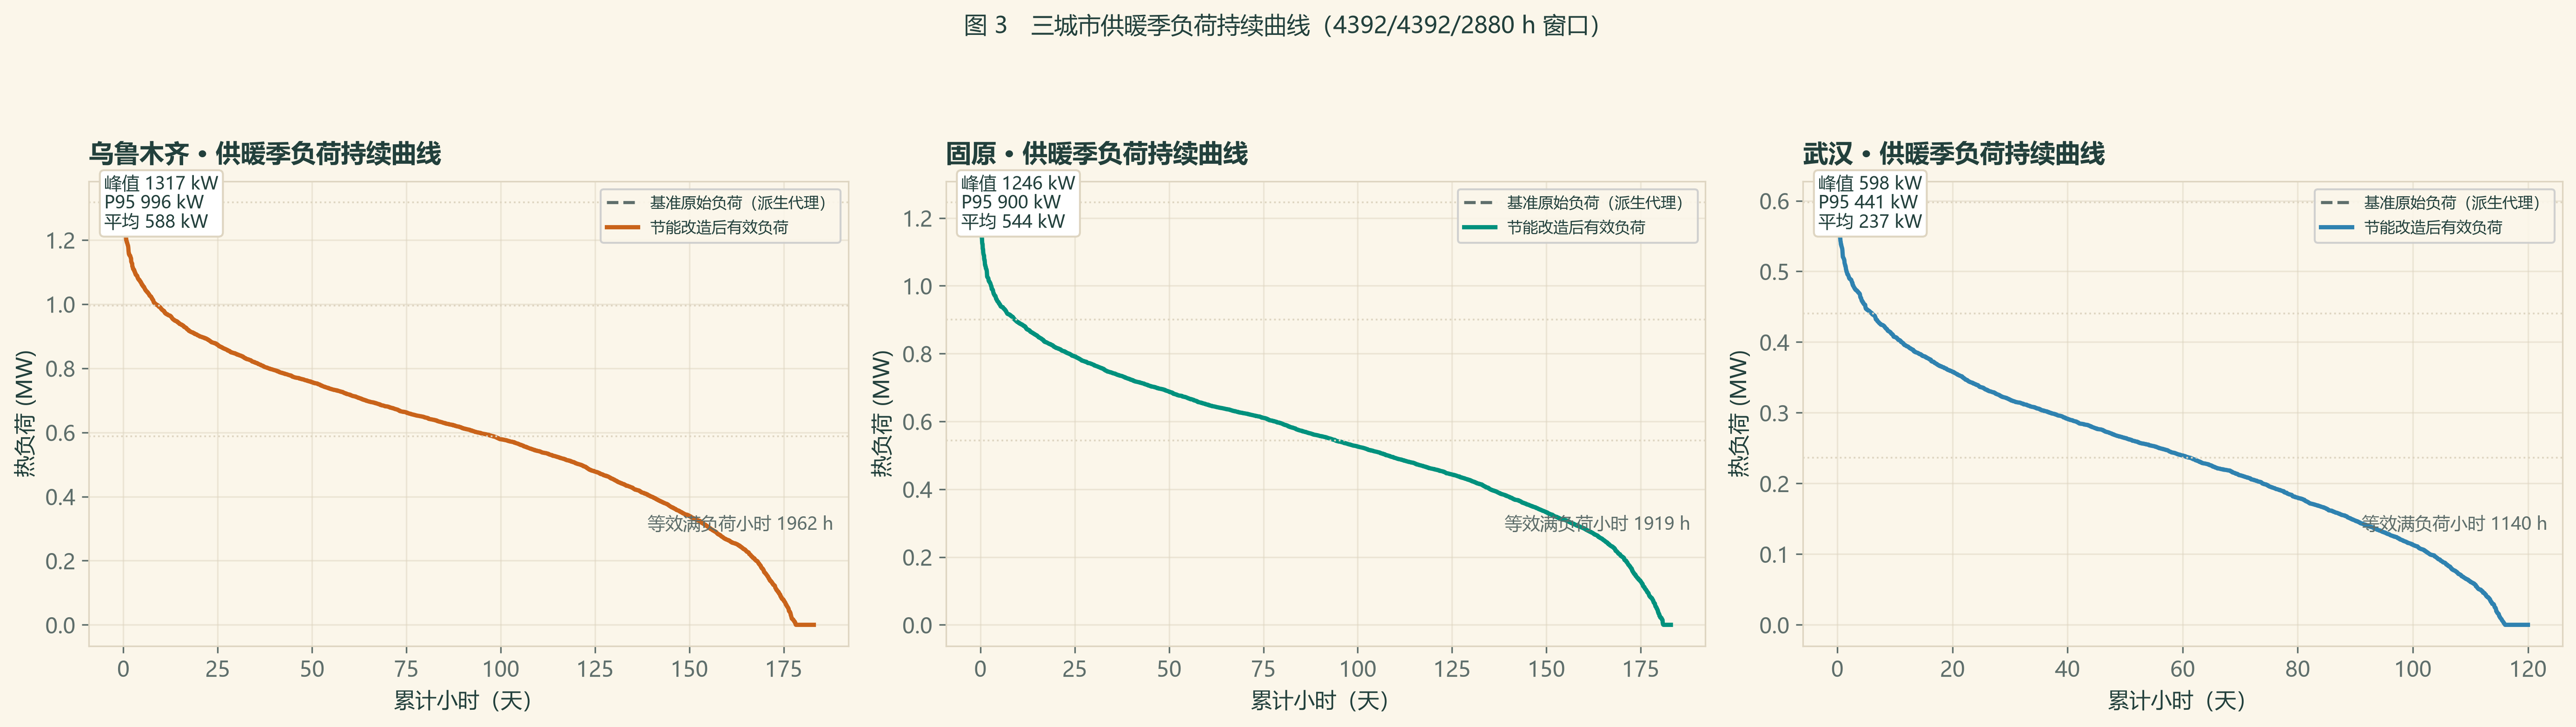
\includegraphics[width=0.98\textwidth,height=0.44\textheight,keepaspectratio,trim=0 0 0 100,clip]{media/code-results/fig03_load_duration_curve.png}
\caption{三城市供暖季负荷持续曲线}
\label{fig:code-load-duration}
\end{figure}

\subsection{模型结构}

模型以建筑逐时负荷为入口，将规划期内的热源建设、设备退役、管网改造、储热配置和配电增容，与供暖季内的热源出力、管网输配、储热充放和建筑热状态统一描述。三个算例均设置3个聚合负荷节点；乌鲁木齐、固原和武汉分别配置7、6、7类热源以及3、2、1条聚合管段。城市层确定资产配置与建设时序，区域层描述热源、管段、换热站和储热之间的能量传输，用户层以聚合节点承载典型建筑负荷与可调节热状态。聚合节点分别对应城市总体边界、区域输配单元和用户侧同类建筑群，不等同于完整城市地理网络。

公用模型内核包含负荷预测、热源转换、节点平衡、管网输配、储热递推、电力平衡和可靠性约束；场景适配模块根据城市的既有资产、资源条件、网络结构和服务需求加载专用约束。整体关系如图\ref{fig:model-cn-overall}所示。

\begin{figure}[H]
\centering
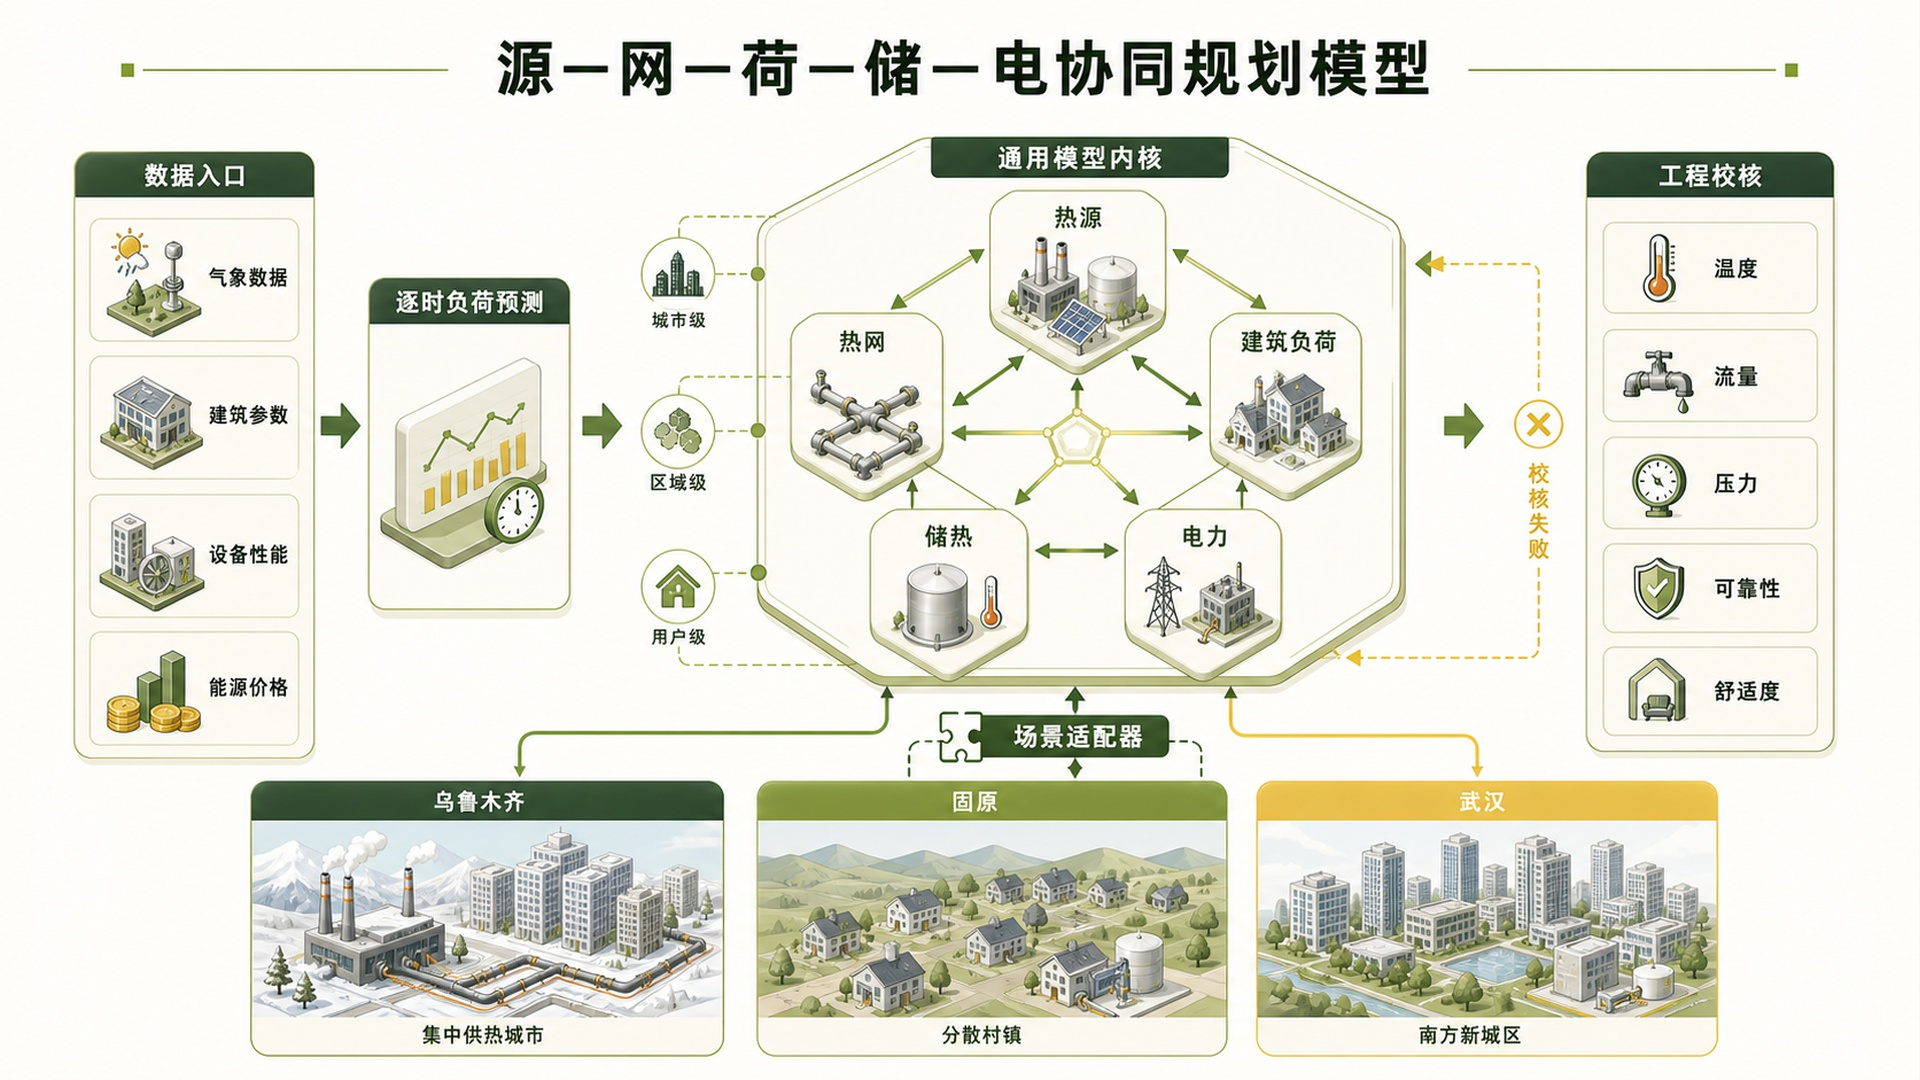
\includegraphics[width=0.76\textwidth,height=0.38\textheight,keepaspectratio]{media/model-cn/01_总体模型框架.jpg}
\caption{协同规划模型框架}
\label{fig:model-cn-overall}
\end{figure}

规划、运行和工程校核采用分层衔接方式。规划层确定建设与容量方案，运行层完成逐时调度；本次数值校核包括热平衡、容量、储热状态、配电边界和失供量检查，工程复核包括温位、关键管段和回水边界。将工程边界自动回写并重新求解属于扩展功能，本次未启用。计算流程如图\ref{fig:model-cn-loop}所示。

\begin{figure}[H]
\centering
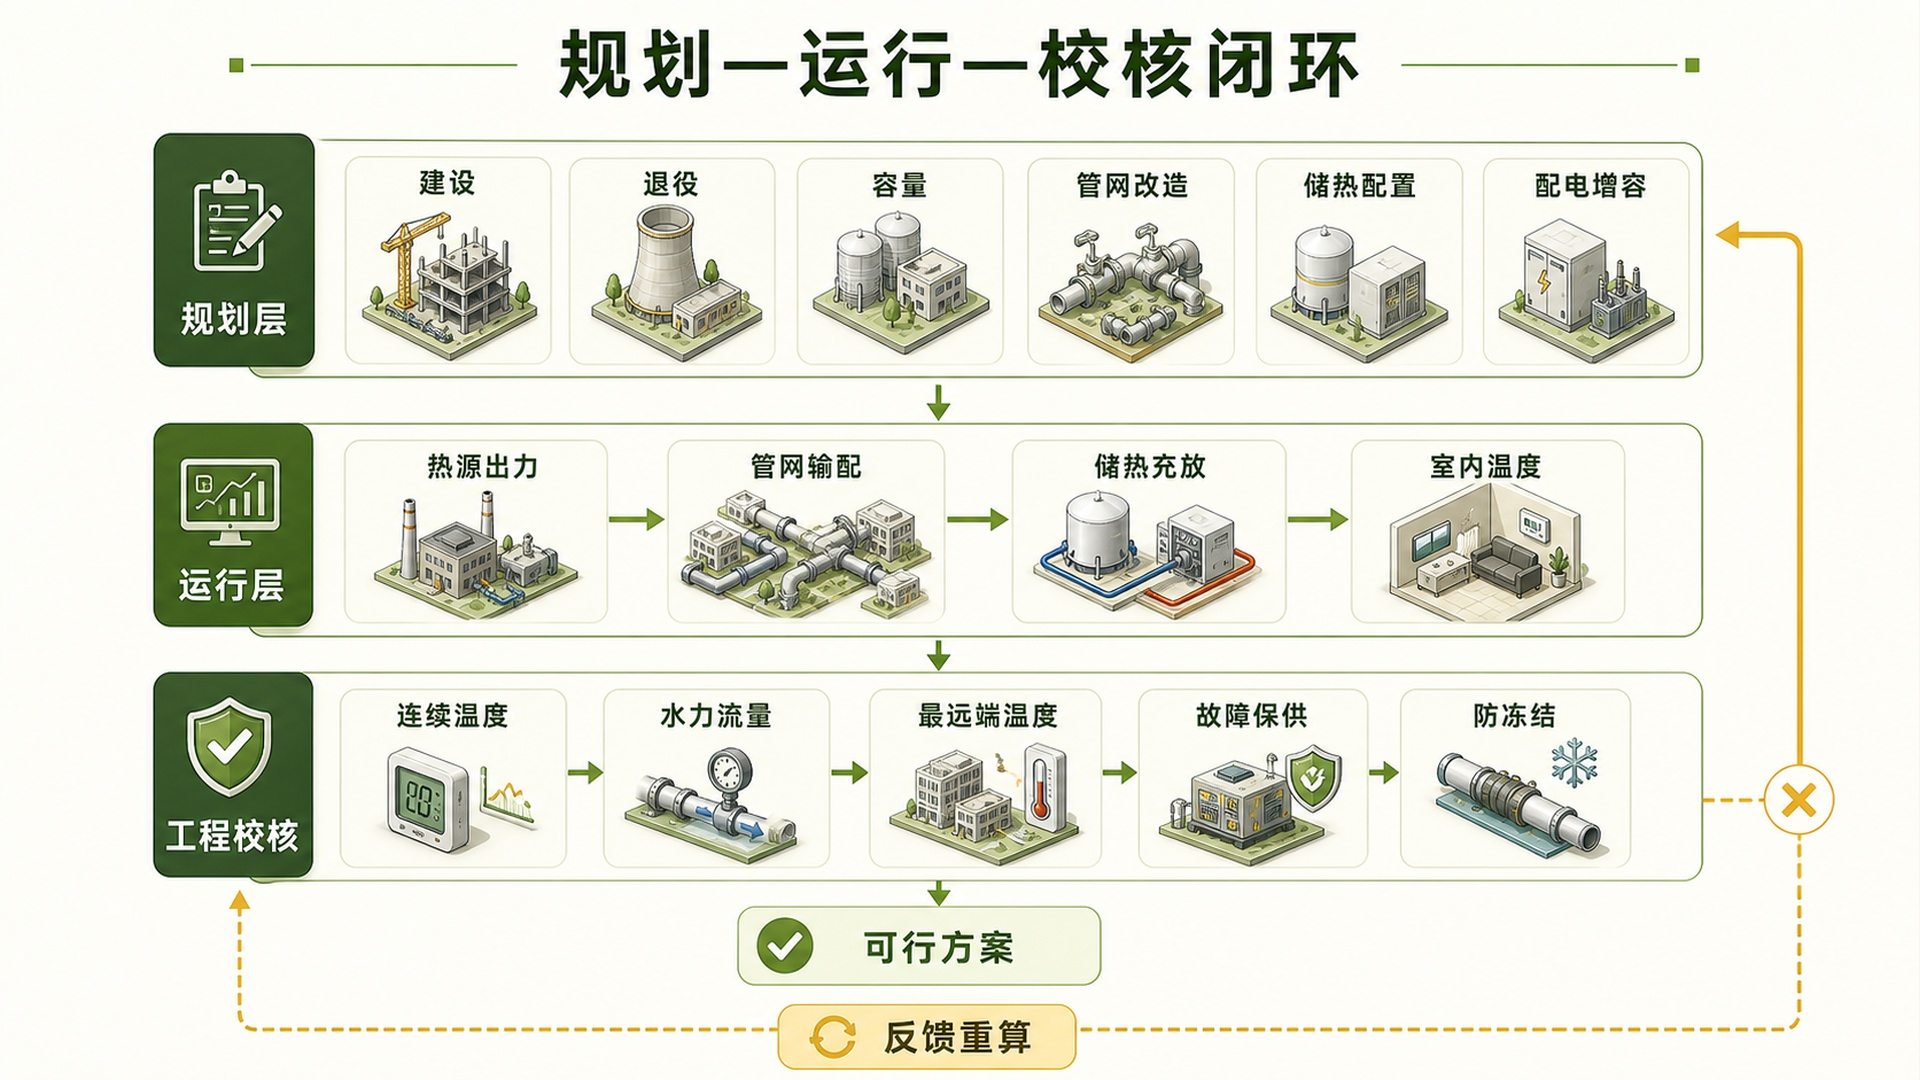
\includegraphics[width=0.76\textwidth,height=0.36\textheight,keepaspectratio]{media/model-cn/05_规划运行校核闭环.jpg}
\caption{规划与校核流程}
\label{fig:model-cn-loop}
\end{figure}

\subsection{建筑负荷}

\subsubsection{负荷分解}

建筑供热负荷由围护结构传热、渗透换气和机械新风热损失构成，同时扣除太阳辐射及人员、设备等内部得热：
\begin{equation}
Q_{b,t}^{\mathrm{load}}=Q_{b,t}^{\mathrm{trans}}+Q_{b,t}^{\mathrm{inf}}+Q_{b,t}^{\mathrm{vent}}-Q_{b,t}^{\mathrm{sol}}-Q_{b,t}^{\mathrm{int}}.
\label{eq:load-decomp}
\end{equation}
围护结构传热与渗透换气损失分别为
\begin{align}
Q_{b,t}^{\mathrm{trans}}&=U_bA_b\left(\theta_{b,t}^{a}-T_t^{\mathrm{out}}\right),\\
Q_{b,t}^{\mathrm{inf}}&=\frac{\rho_ac_an_b^{\mathrm{inf}}V_b}{3.6\times10^6}
\left(\theta_{b,t}^{a}-T_t^{\mathrm{out}}\right).
\end{align}
式中，$U_b$为综合传热系数，$A_b$为围护结构面积，$n_b^{\mathrm{inf}}$为换气次数（次/h），$V_b$为建筑体积；当$\rho_a$取kg/m$^3$、$c_a$取J/(kg$\cdot$K)时，除以$3600$完成小时换算，再除以$1000$得到kW。负荷分解关系见图\ref{fig:model-cn-load}。

\begin{figure}[H]
\centering
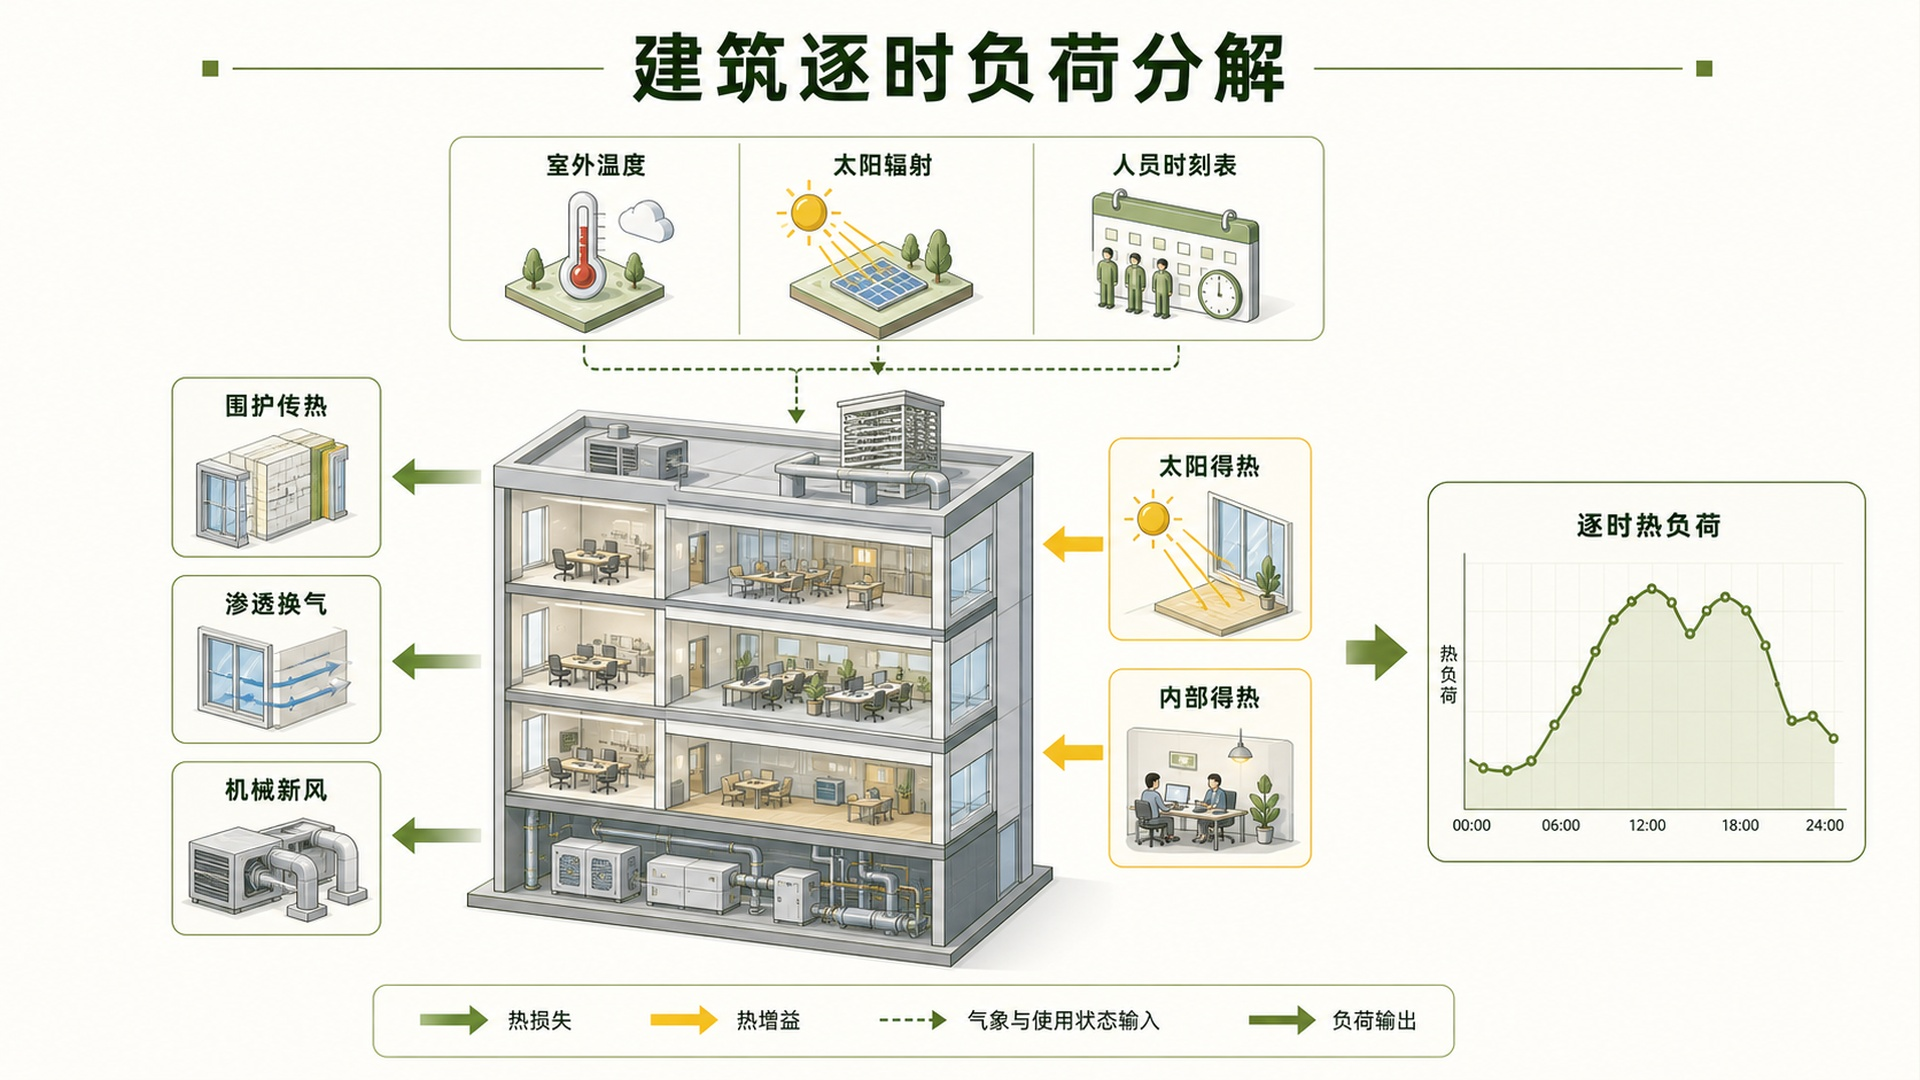
\includegraphics[width=0.76\textwidth,height=0.36\textheight,keepaspectratio]{media/model-cn/02_建筑逐时负荷分解.jpg}
\caption{建筑逐时负荷分解}
\label{fig:model-cn-load}
\end{figure}

\subsubsection{热惯性模型}

本次代码采用单一等效热状态表示用户侧热惯性。令$E_{b,t}$为相对基准状态的蓄热量，$C_b$为聚合节点等效热容，$q_{b,t}^{+}$和$q_{b,t}^{-}$分别表示相对基准的负荷增加量和削减量，$\lambda_b$为每个时间步的衰减率，则
\begin{align}
E_{b,t}&=(1-\lambda_b)E_{b,t-1}+\left(q_{b,t}^{+}-q_{b,t}^{-}\right)\Delta t,\\
\Delta\theta_{b,t}&=\frac{E_{b,t}}{C_b},\qquad \Delta t=1~\mathrm h.
\end{align}
式中$\lambda_b$取该节点的逐时恢复损失率，$|\Delta\theta_{b,t}|$受最大温度偏移约束；需求响应仅在允许窗口内转移负荷，并满足全窗口能量守恒。需要说明该状态量的作用位置：基准轨迹由节点外生负荷曲线给出，$E_{b,t}$不回馈到节点热平衡的显性需求项，而是用于记录移峰量与舒适偏差惩罚，因此它描述的是相对基准的调节裕度，不是独立的室温状态。

三个场景主链采用上述单一等效热状态，不进行房间级温度模拟。图\ref{fig:model-cn-2r2c}保留原有建筑热惯性结构示意，其两节点结构用于说明围护与室内空气的分层热容，与上式的聚合等效热状态不是同一个模型；凡启用楼栋级室温递推的算例，其状态方程按式\eqref{eq:alg-building}单独登记，两者不互换。

\begin{figure}[H]
\centering
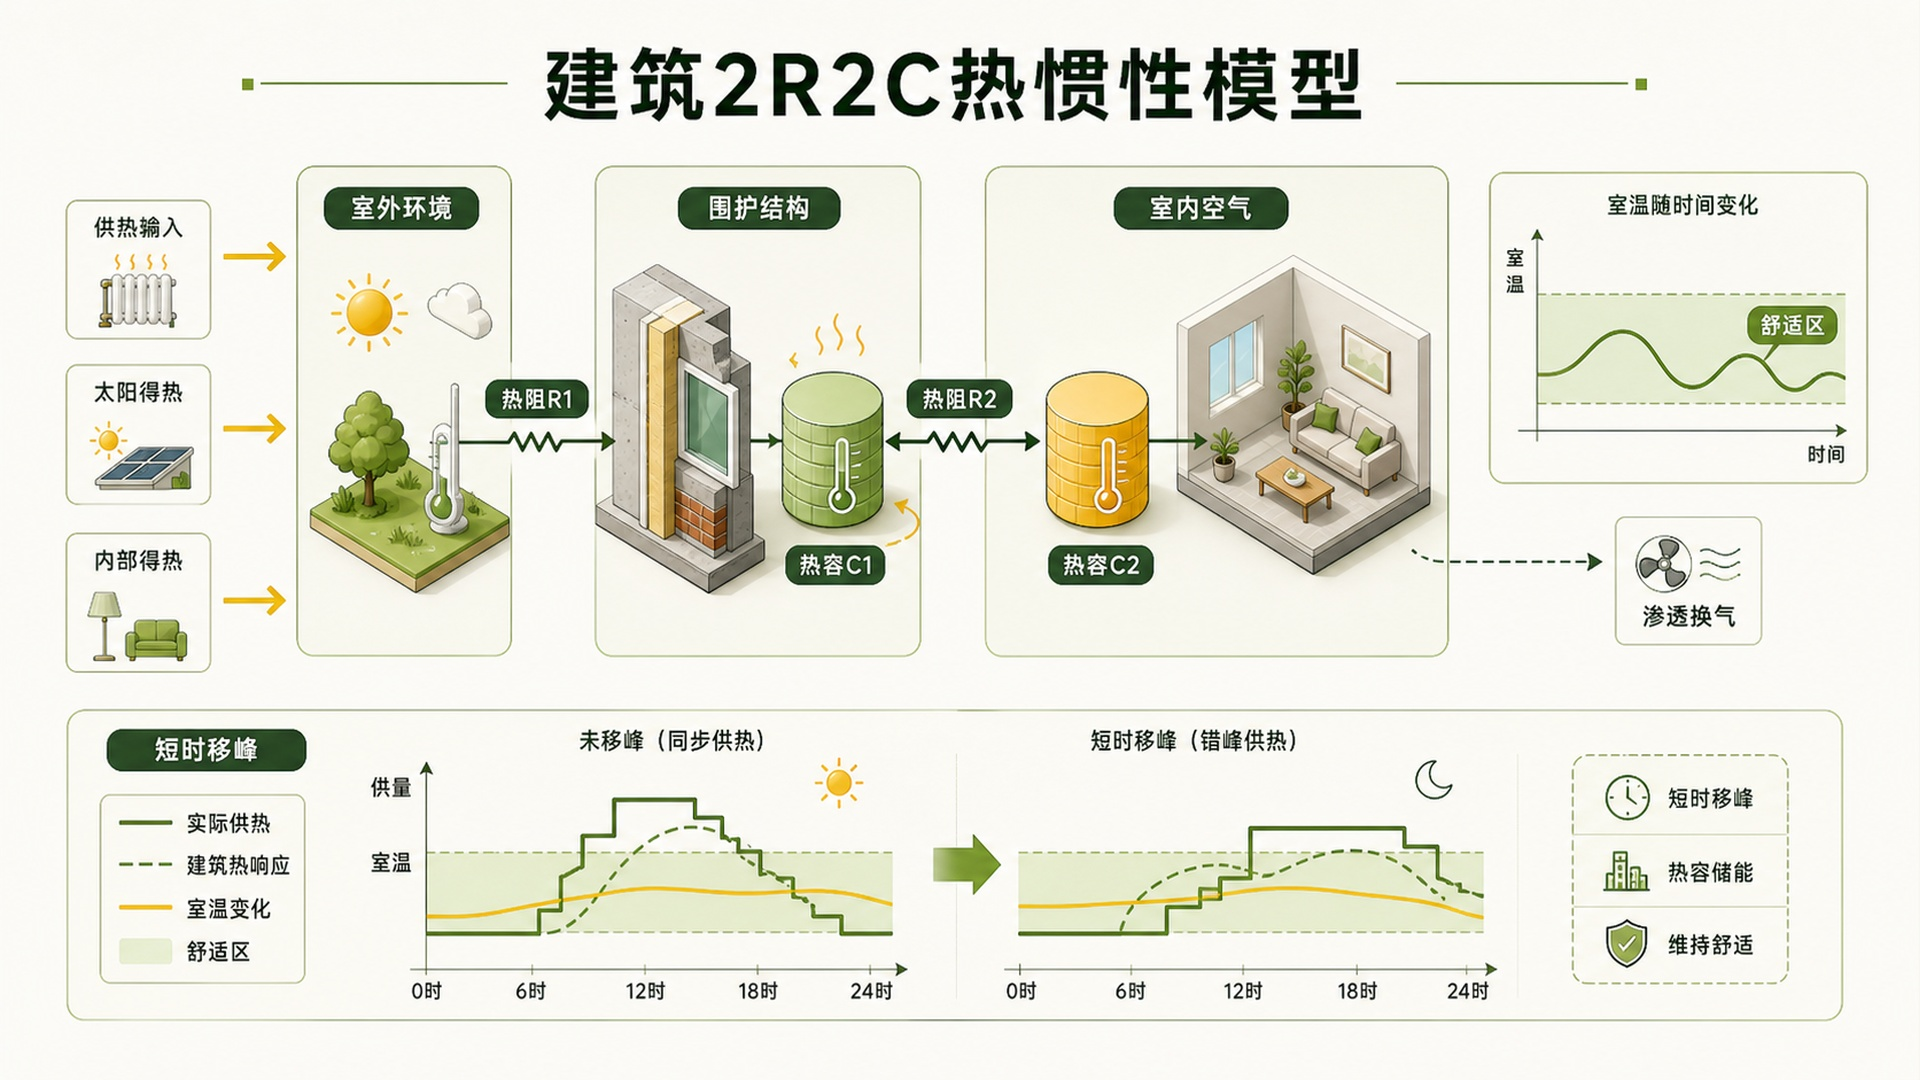
\includegraphics[width=0.76\textwidth,height=0.36\textheight,keepaspectratio]{media/model-cn/03_建筑2R2C热惯性.jpg}
\caption{建筑2R2C模型}
\label{fig:model-cn-2r2c}
\end{figure}

\subsection{协同约束}

\subsubsection{容量与出力}

设备在规划阶段的可用容量由既有、新建和退役容量共同决定：
\begin{equation}
K_{k,y}=K_k^{\mathrm{exist}}+\sum_{\tau\leq y}K_{k,\tau}^{\mathrm{new}}-\sum_{\tau\leq y}K_{k,\tau}^{\mathrm{ret}}.
\end{equation}
热源逐时出力满足
\begin{equation}
\underline Q_k u_{k,t}\leq Q_{k,t}\leq \overline Q_k u_{k,t},
\qquad Q_{k,t}\leq a_{k,t}K_{k,y},
\end{equation}
其中$u_{k,t}$为启停状态，$a_{k,t}$为可用率。锅炉和热泵的能量转换关系分别为
\begin{equation}
Q_{k,t}^{\mathrm{boiler}}=\eta_k^{\mathrm{boiler}}F_{k,t}^{\mathrm{fuel}},
\qquad Q_{k,t}^{\mathrm{HP}}=COP_{k,t}P_{k,t}^{\mathrm{HP}}.
\end{equation}

\subsubsection{热量平衡}

对节点$n$、温位$g$和时刻$t$，热源输入、上游来热和储热放热应等于用户负荷、储热充热和下游送热：
\begin{multline}
\sum_k Q_{k,n,g,t}+\sum_{e\in\delta^-(n)}\eta_eF_{e,g,t}+\sum_sQ_{s,n,g,t}^{\mathrm{dis}}\\
=D_{n,g,t}+\sum_sQ_{s,n,g,t}^{\mathrm{ch}}+\sum_{e\in\delta^+(n)}F_{e,g,t}.
\label{eq:node-heat-balance}
\end{multline}
该约束按节点、温位和时段分别建立，避免使用全系统总量平衡掩盖局部输配不足。源、网、荷、储、电之间的关系见图\ref{fig:model-cn-unified}。

\begin{figure}[H]
\centering
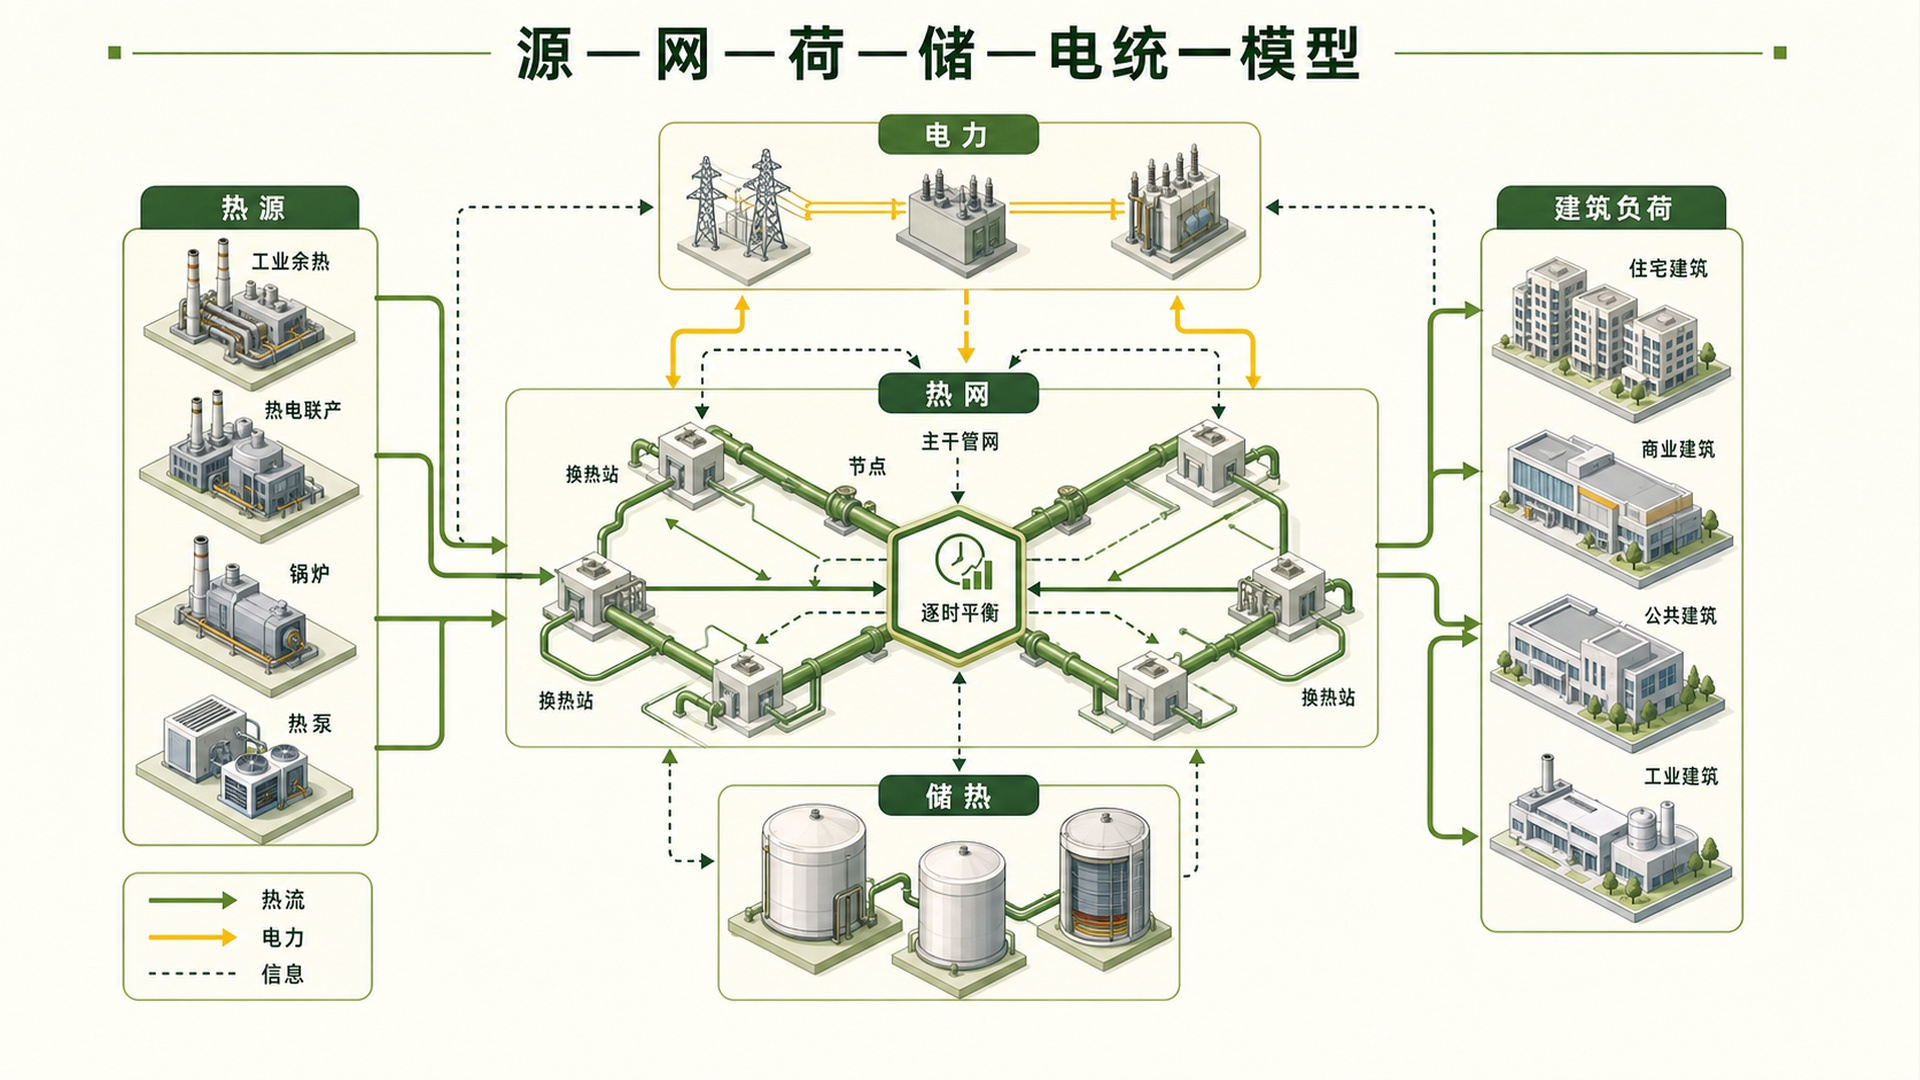
\includegraphics[width=0.76\textwidth,height=0.37\textheight,keepaspectratio]{media/model-cn/04_源网荷储电统一模型.jpg}
\caption{多能流协同关系}
\label{fig:model-cn-unified}
\end{figure}

\subsubsection{温位与管网}

热源最低供水温度应满足用户温位和换热端差要求：
\begin{equation}
T_k^{\mathrm{src,min}}\geq T_g^{\mathrm{sup}}+\Delta T^{\mathrm{hx}}.
\end{equation}
主模型采用固定温差将热流与质量流量关联：
\begin{equation}
F_{e,g,t}=c_p\Delta T_g\dot m_{e,g,t},
\qquad |F_{e,t}|\leq F_e^{\mathrm{exist}}+\sum_d\overline F_{e,d}z_{e,d}.
\end{equation}
温位不匹配的热源不得直接承担高温负荷，需要通过热泵等设备提升温度。梯级利用关系见图\ref{fig:model-cn-grade}。

\begin{figure}[H]
\centering
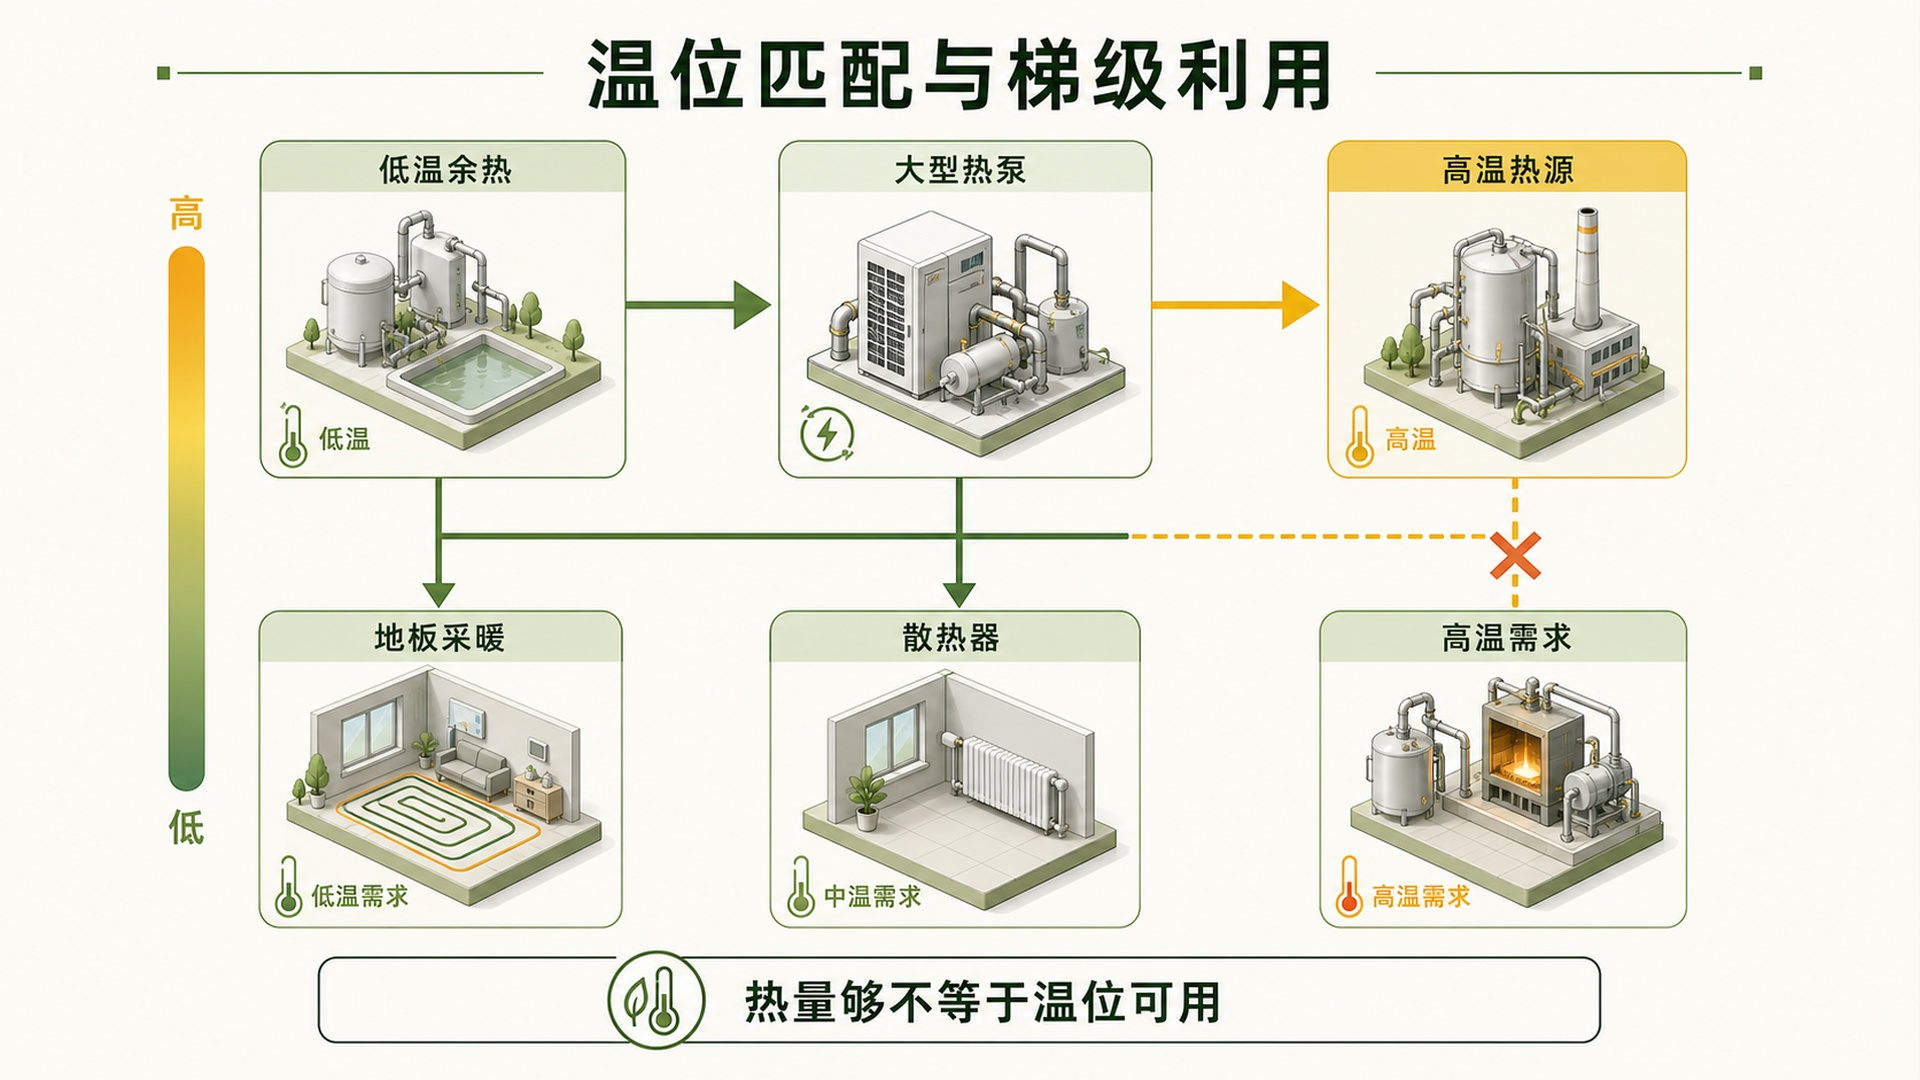
\includegraphics[width=0.76\textwidth,height=0.35\textheight,keepaspectratio]{media/model-cn/06_温位匹配与梯级利用.jpg}
\caption{温位匹配与梯级利用}
\label{fig:model-cn-grade}
\end{figure}

\subsubsection{储热与电力}

储热状态按时段递推：
\begin{equation}
E_{s,t}=(1-\mu_s)E_{s,t-1}+\eta_s^{\mathrm{ch}}Q_{s,t}^{\mathrm{ch}}\Delta t
-\frac{Q_{s,t}^{\mathrm{dis}}\Delta t}{\eta_s^{\mathrm{dis}}}.
\label{eq:storage-state}
\end{equation}
热泵、电锅炉、循环泵和储电设备共同进入节点电力平衡：
\begin{multline}
P_{n,t}^{\mathrm{imp}}+P_{n,t}^{\mathrm{RES}}+P_{n,t}^{\mathrm{CHP}}+P_{n,t}^{\mathrm{bat,dis}}\\
=P_{n,t}^{\mathrm{base}}+P_{n,t}^{\mathrm{HP}}+P_{n,t}^{\mathrm{EB}}
+P_{n,t}^{\mathrm{pump}}+P_{n,t}^{\mathrm{bat,ch}}+P_{n,t}^{\mathrm{exp}}.
\end{multline}
储热充放时序与配电峰值的关系见图\ref{fig:model-cn-storage-grid}。

\begin{figure}[H]
\centering
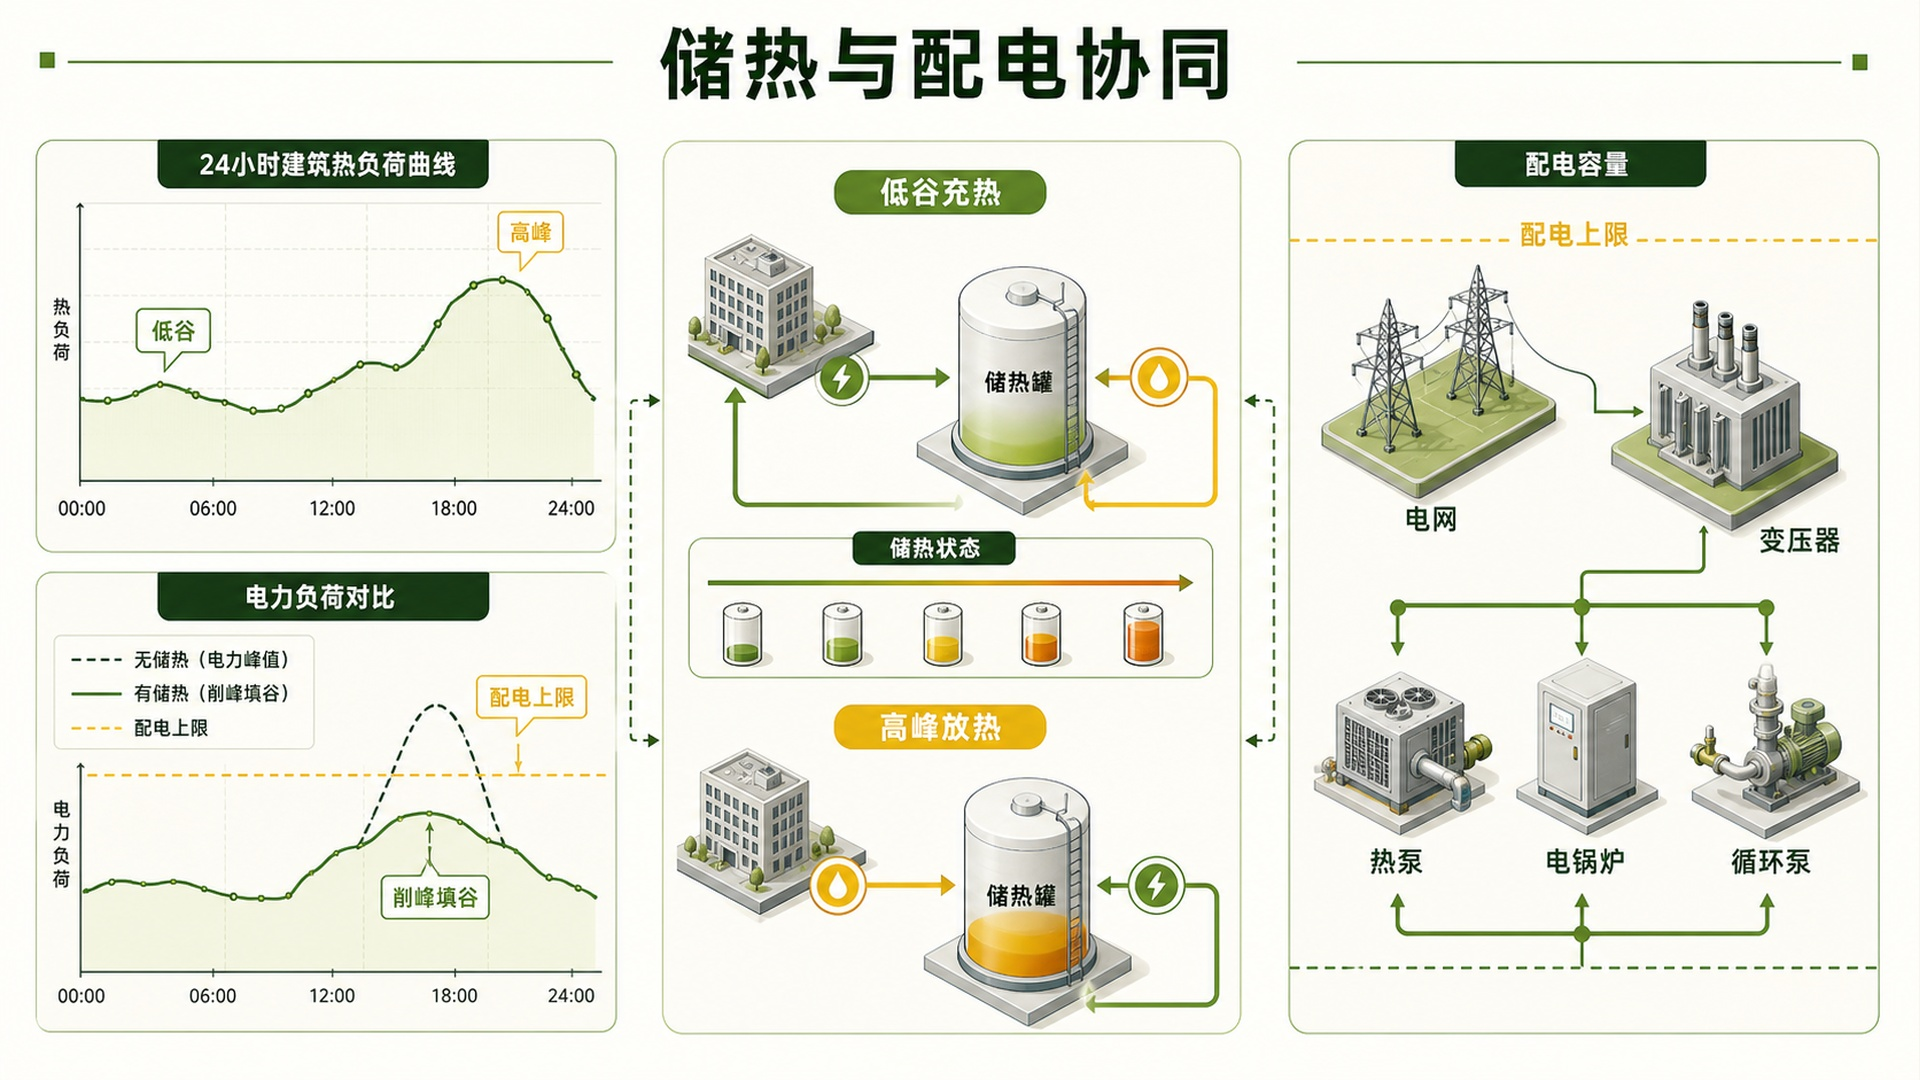
\includegraphics[width=0.76\textwidth,height=0.35\textheight,keepaspectratio]{media/model-cn/07_储热与配电协同.jpg}
\caption{储热与配电协同}
\label{fig:model-cn-storage-grid}
\end{figure}

\subsubsection{目标与可靠性}

模型以生命周期净成本$F^{\mathrm{cost}}$最小为基础目标，并通过$\varepsilon$约束控制碳排放。投资按5\%折现率和20年寿命折算为等年值，目标函数写为
\begin{align}
\min F^{\mathrm{cost}}={}&C^{\mathrm{ann,inv}}+C^{\mathrm{energy}}+C^{\mathrm{carbon}}
+C^{\mathrm{om}}+C^{\mathrm{pen}},\\
C^{\mathrm{ann,inv}}={}&\frac{r(1+r)^{20}}{(1+r)^{20}-1}C^{\mathrm{inv}},
\qquad r=5\%,\\
&F^{\mathrm{CO_2}}\leq\varepsilon_C.
\end{align}
其中$C^{\mathrm{energy}}$为能源费，$C^{\mathrm{carbon}}$为碳费，$C^{\mathrm{om}}$为运维费，$C^{\mathrm{pen}}$为火用失配与舒适偏差惩罚。实际现金成本仅包含发生的能源、运维和碳费用，不与惩罚项混合解释。
失供率定义为
\begin{equation}
U^{\mathrm{un}}=\frac{\sum_tQ_t^{\mathrm{un}}}{\sum_tD_t}\leq\overline U.
\end{equation}
推荐方案取$\overline U=0$。室温、设备出力、温位、管网、储热和配电容量均作为硬约束，成本与碳排放在可行域内比较。约束关系见图\ref{fig:model-cn-objective}。

\begin{figure}[H]
\centering
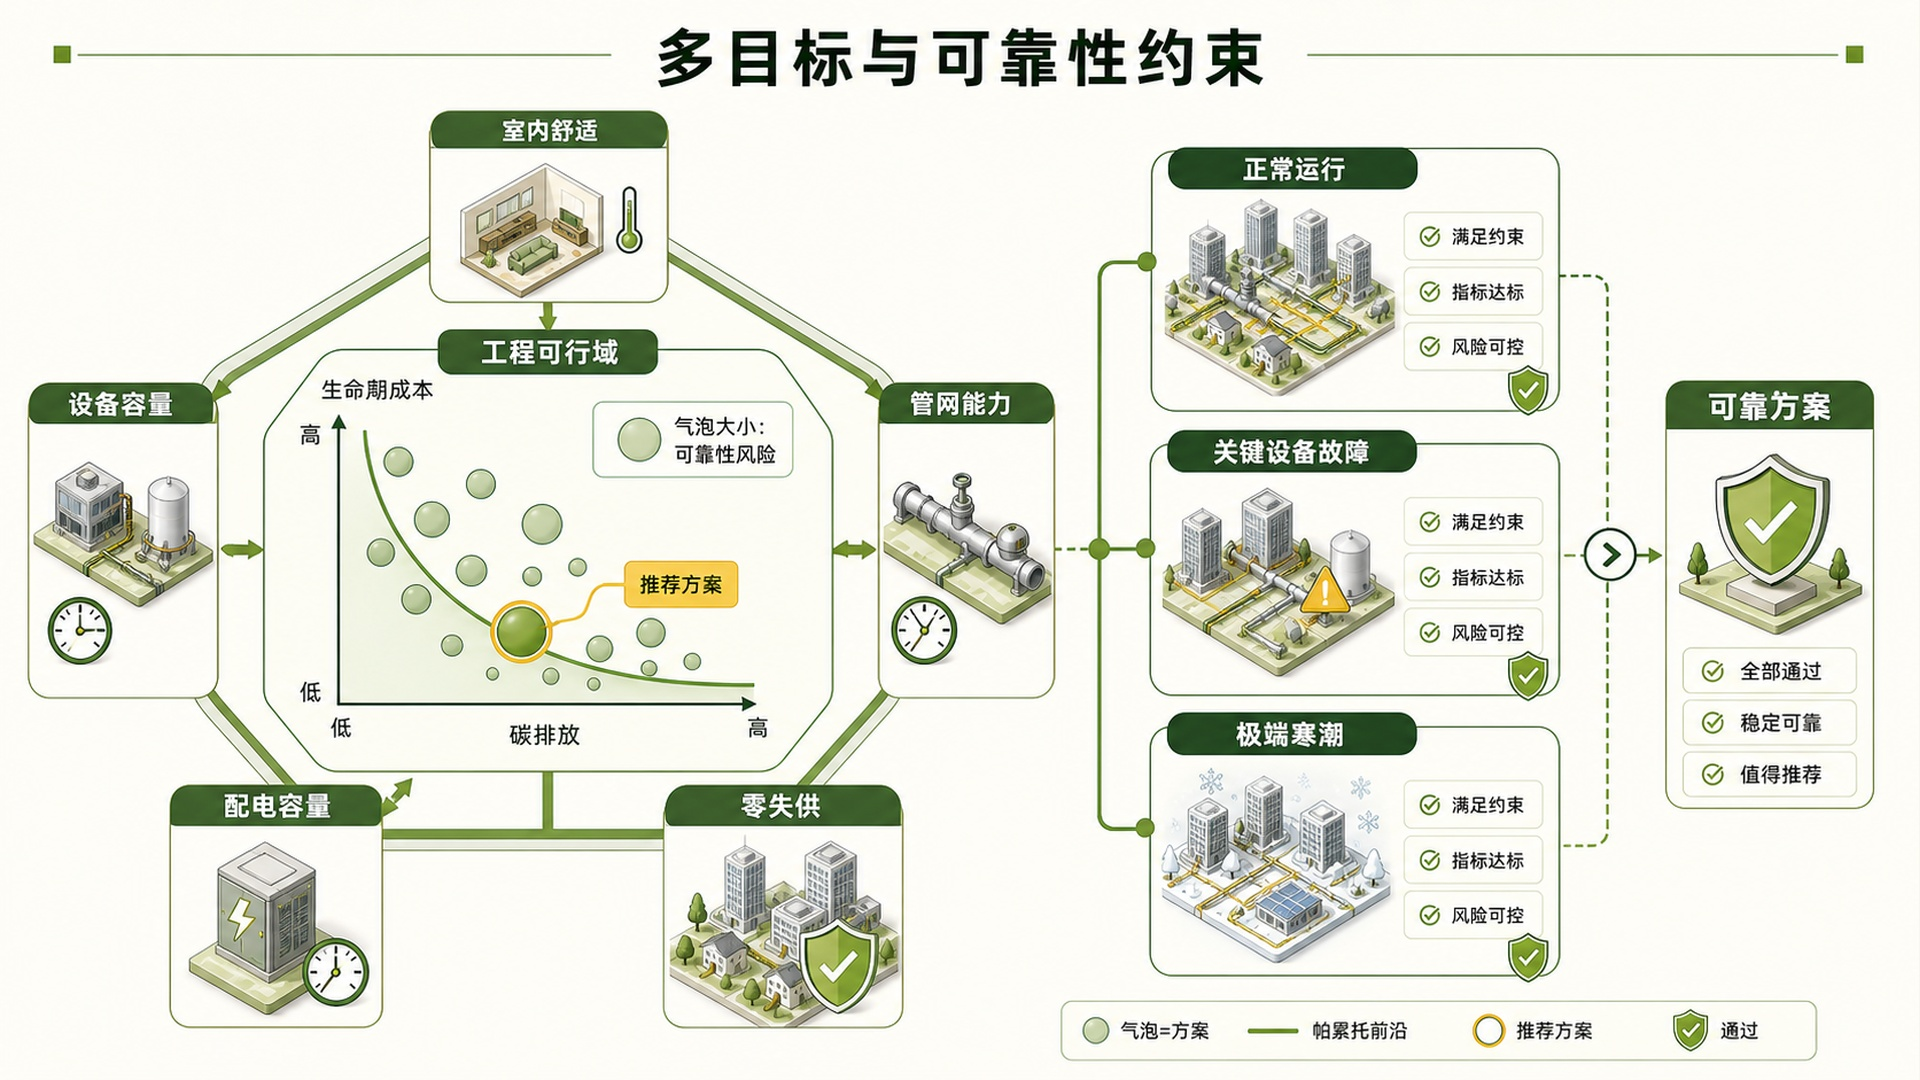
\includegraphics[width=0.76\textwidth,height=0.36\textheight,keepaspectratio]{media/model-cn/08_多目标与可靠性约束.jpg}
\caption{目标函数与可靠性约束}
\label{fig:model-cn-objective}
\end{figure}

\subsection{场景适配}

\subsubsection{乌鲁木齐场景}

乌鲁木齐以既有热电联产、骨干管网和换热站为基础，联合确定燃煤热源退役、工业余热接入、大型热泵、清洁调峰热源、储热及管网降温方案。退役容量必须由清洁热源、储热有效容量和备用容量共同补足：
\begin{equation}
K_{\mathrm{coal},y}^{\mathrm{ret}}\leq K_y^{\mathrm{clean,new}}+K_y^{\mathrm{storage,credit}}+K_y^{\mathrm{reserve}}.
\end{equation}
工业余热满足$0\leq Q_t^{\mathrm{waste}}\leq\overline Q_t^{\mathrm{waste}}$，温位不足时通过热泵升温。模型结构见图\ref{fig:model-cn-urumqi}。

\begin{figure}[H]
\centering
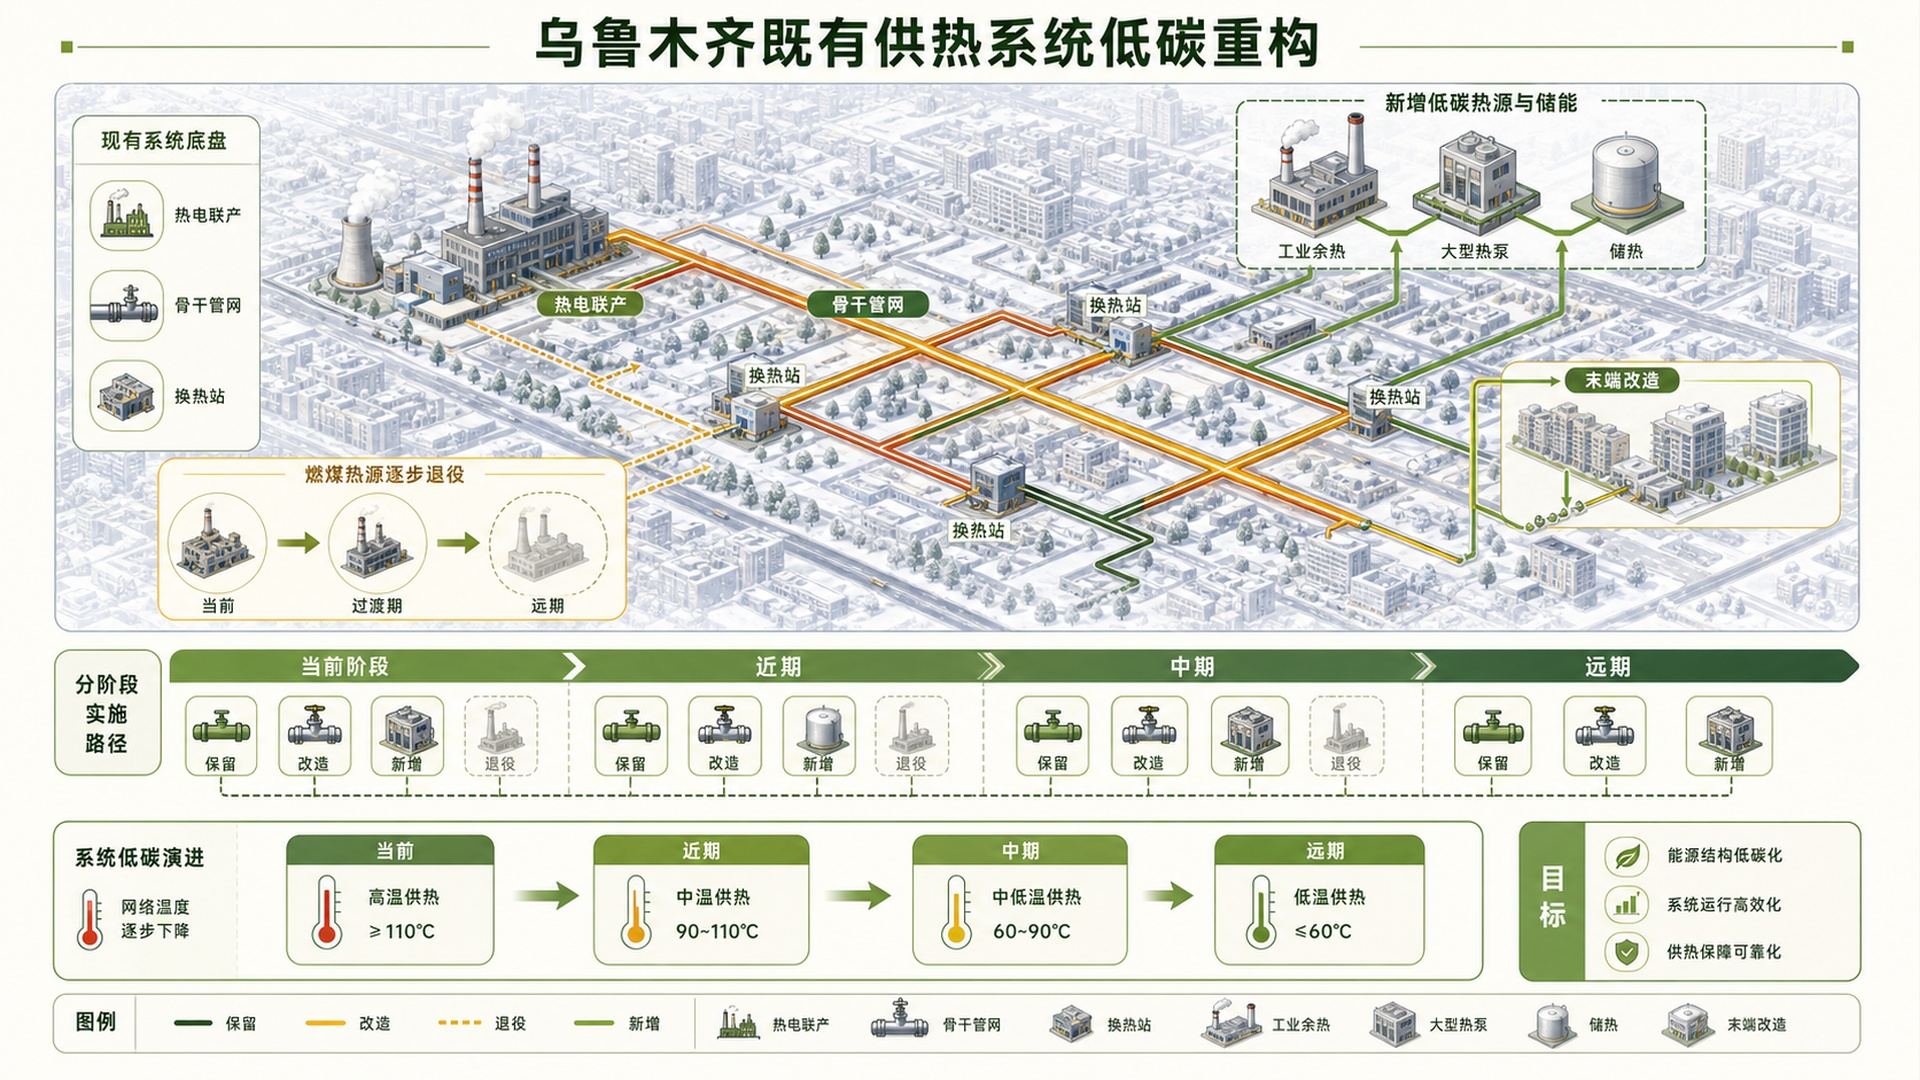
\includegraphics[width=0.77\textwidth,height=0.38\textheight,keepaspectratio]{media/model-cn/09_乌鲁木齐低碳重构.jpg}
\caption{乌鲁木齐低碳重构}
\label{fig:model-cn-urumqi}
\end{figure}

候选方案确定后，校核最远换热站供水温度、关键管段流量、回水温度、供回水温差、热源N-1、寒潮零失供以及管网降温与建筑末端改造的协调关系，见图\ref{fig:model-cn-urumqi-check}。详细约束列于附录1。

\begin{figure}[H]
\centering
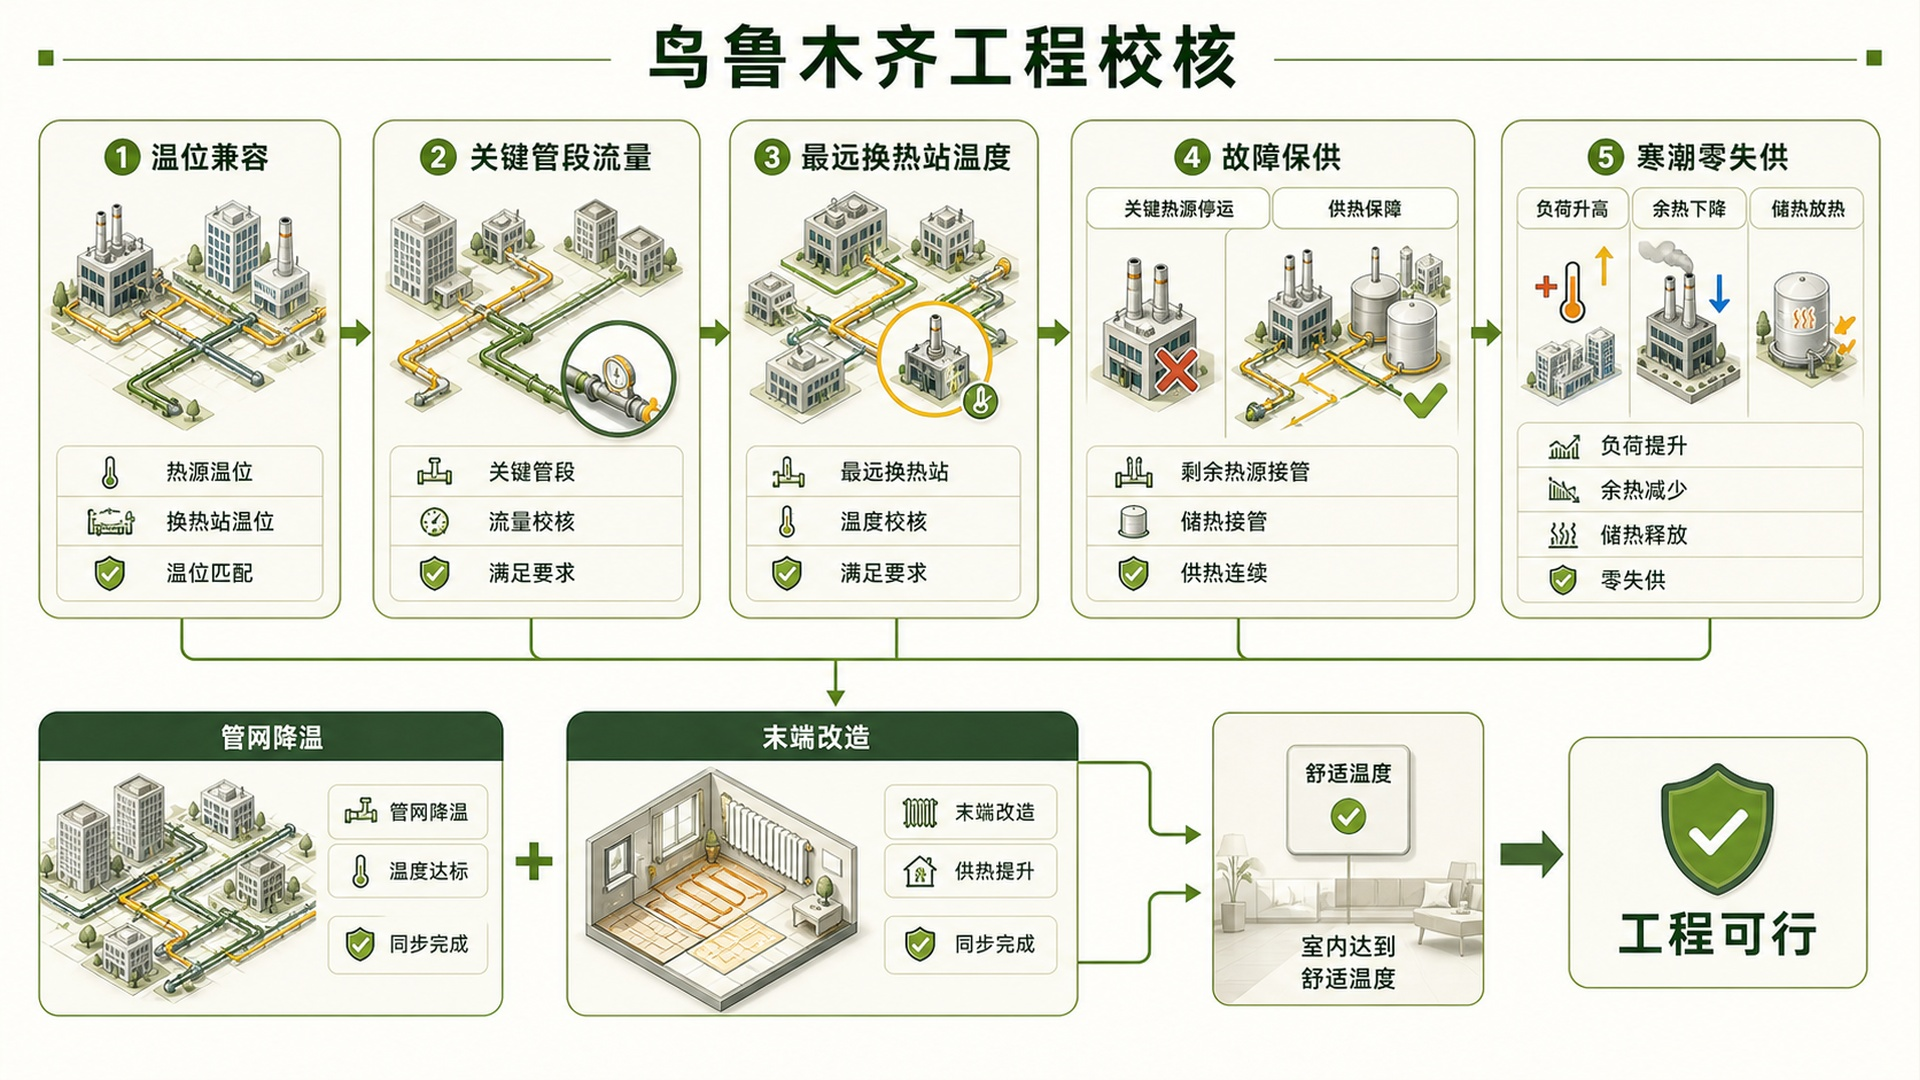
\includegraphics[width=0.76\textwidth,height=0.35\textheight,keepaspectratio]{media/model-cn/10_乌鲁木齐工程校核.jpg}
\caption{乌鲁木齐工程校核}
\label{fig:model-cn-urumqi-check}
\end{figure}

\subsubsection{固原场景}

固原以村镇、片区和区域微网为基本单元，联合优化热源选址、用户分配、微网拓扑、设备容量及燃料供应。用户分配和服务半径满足
\begin{equation}
\sum_i x_{i,b}=1,\qquad x_{i,b}\leq z_i^{\mathrm{site}},\qquad
d_{i,b}x_{i,b}\leq\overline d_i,
\end{equation}
热源容量满足$\sum_bD_b^{\mathrm{peak}}x_{i,b}\leq K_i$。空间组织和技术配置见图\ref{fig:model-cn-guyuan}。

\begin{figure}[H]
\centering
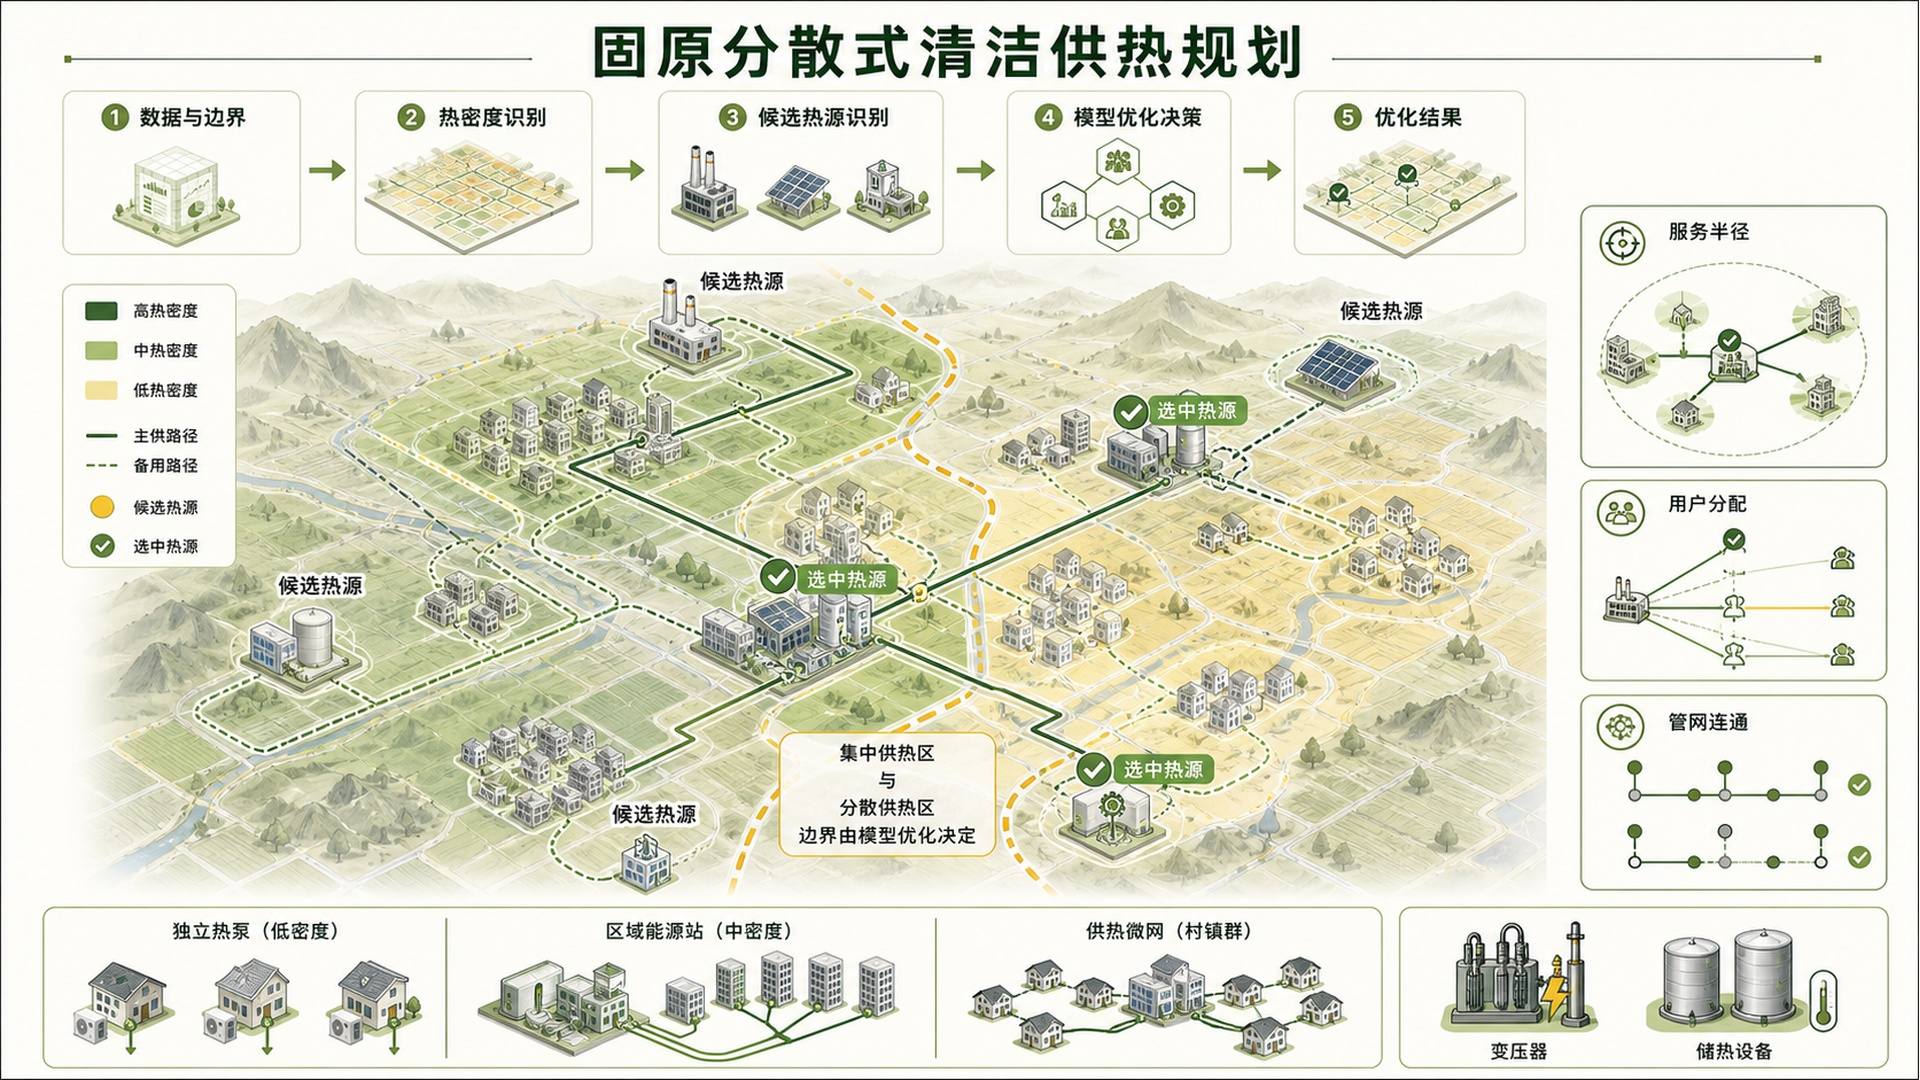
\includegraphics[width=0.77\textwidth,height=0.38\textheight,keepaspectratio]{media/model-cn/11_固原分散供热规划.jpg}
\caption{固原分散供热规划}
\label{fig:model-cn-guyuan}
\end{figure}

生物质燃料按到货、库存和消耗逐时递推，并在电网或单一热源故障下检查关键用户保供。燃料供应与孤岛运行关系见图\ref{fig:model-cn-guyuan-risk}，详细约束列于附录1。

\begin{figure}[H]
\centering
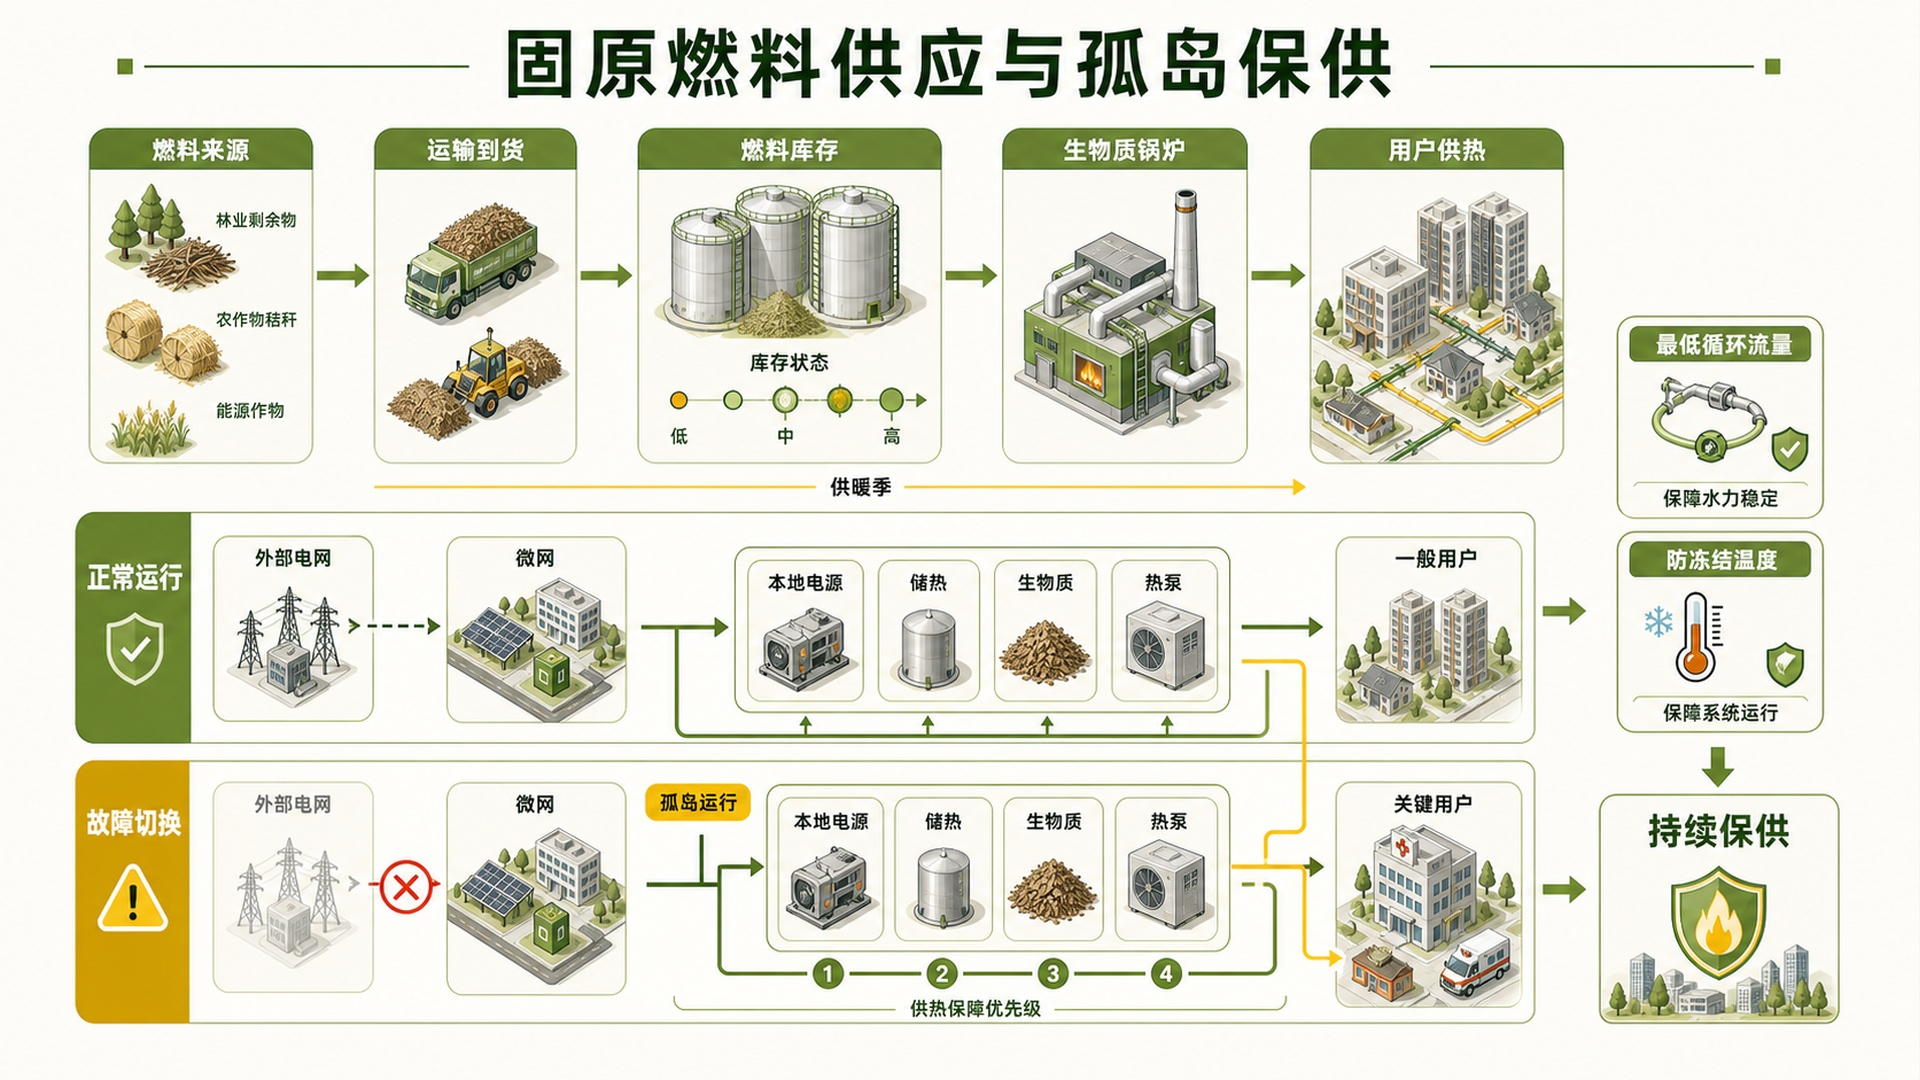
\includegraphics[width=0.76\textwidth,height=0.35\textheight,keepaspectratio]{media/model-cn/12_固原燃料与孤岛保供.jpg}
\caption{固原燃料与孤岛保供}
\label{fig:model-cn-guyuan-risk}
\end{figure}

\subsubsection{武汉场景}

武汉以楼栋和小区为主要空间单元，在独立楼宇、区域能源站、低温热网和第五代区域供热供冷系统之间进行选择：
\begin{equation}
z_i^{\mathrm{building}}+z_i^{\mathrm{station}}+z_i^{\mathrm{LTN}}+z_i^{\mathrm{5GDHC}}=1.
\end{equation}
四类形态的适用边界见图\ref{fig:model-cn-wuhan-types}。

\begin{figure}[H]
\centering
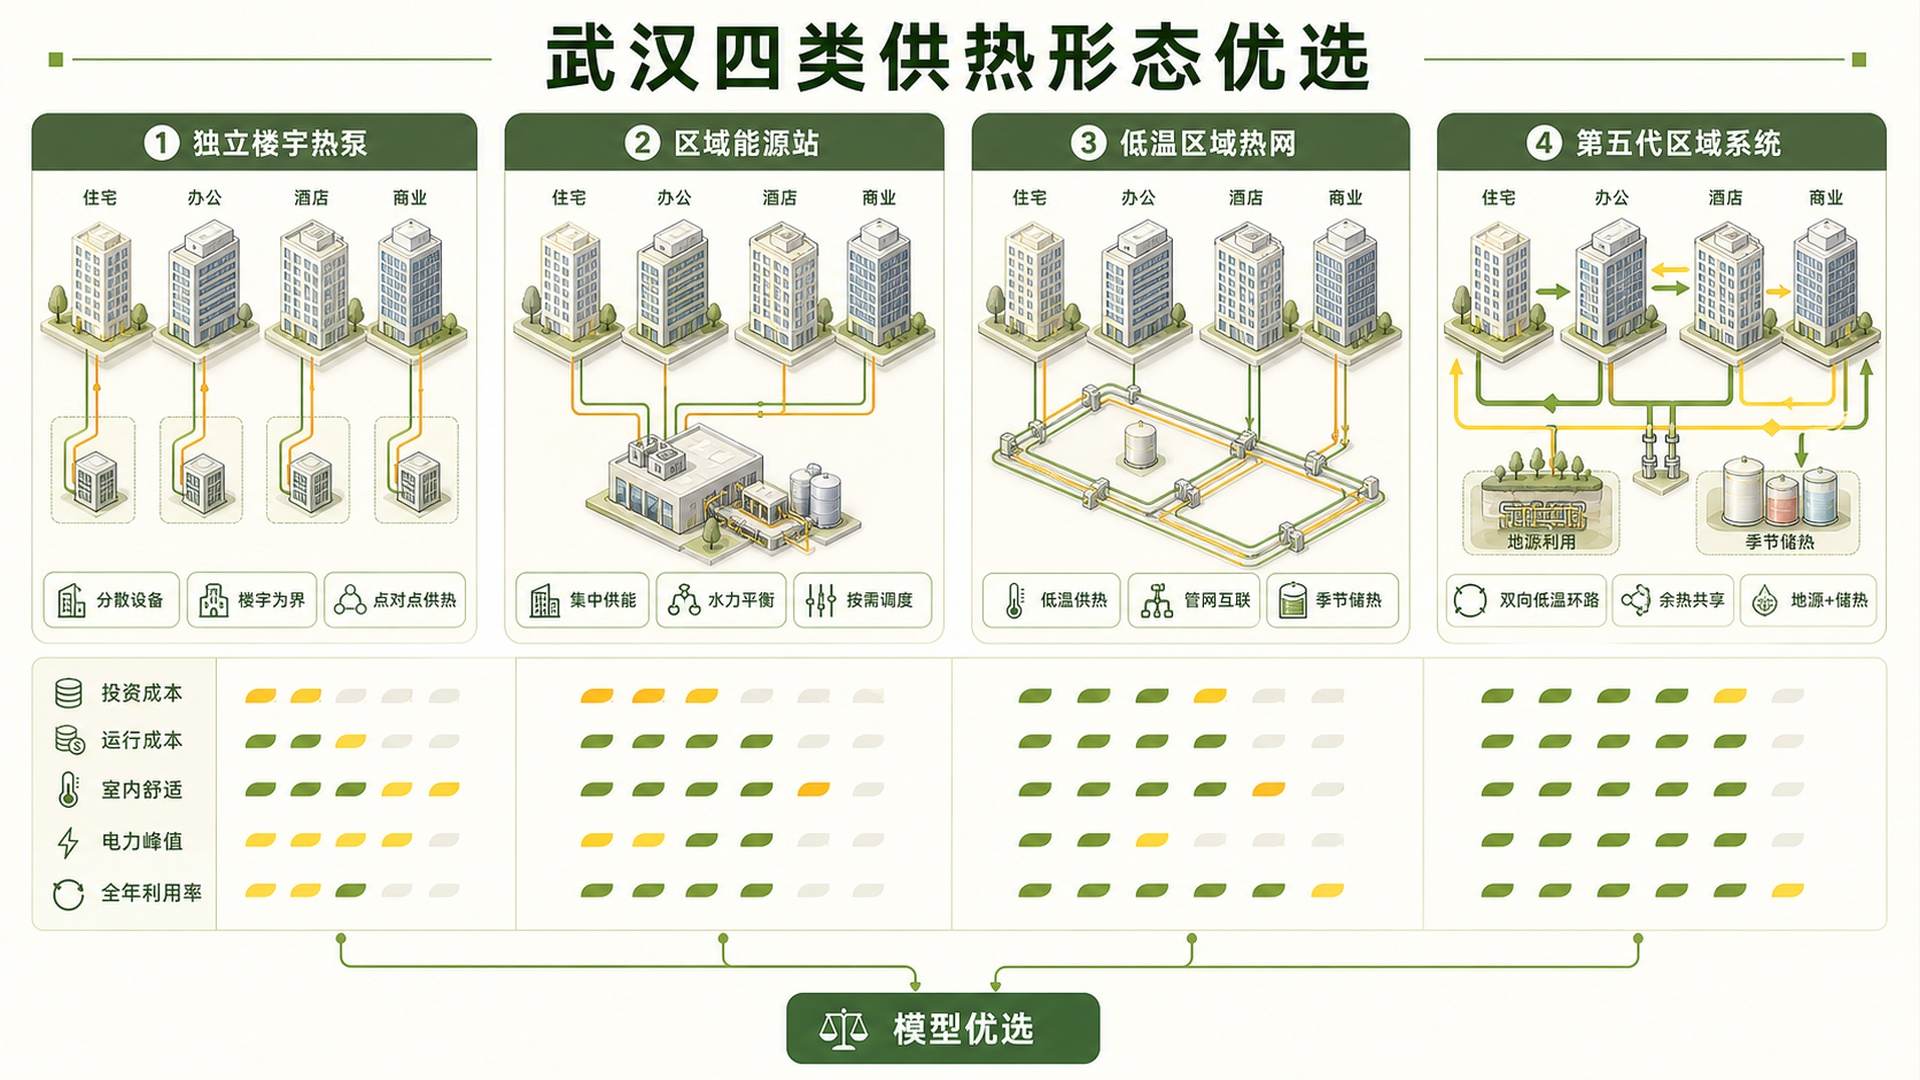
\includegraphics[width=0.76\textwidth,height=0.35\textheight,keepaspectratio]{media/model-cn/13_武汉四类供热形态.jpg}
\caption{武汉供热形态}
\label{fig:model-cn-wuhan-types}
\end{figure}

武汉场景同时考虑供热、供冷、生活热水、间歇预热、温湿度、新风、结露、除霜、地源年度平衡、噪声和楼栋配电容量。低温末端表面温度应高于露点并保留安全裕度：
\begin{equation}
T_{b,t}^{\mathrm{surface}}\geq T_{b,t}^{\mathrm{dew}}+\Delta T^{\mathrm{safe}}.
\end{equation}
主要约束见图\ref{fig:model-cn-wuhan-quality}，详细表达列于附录1。

\begin{figure}[H]
\centering
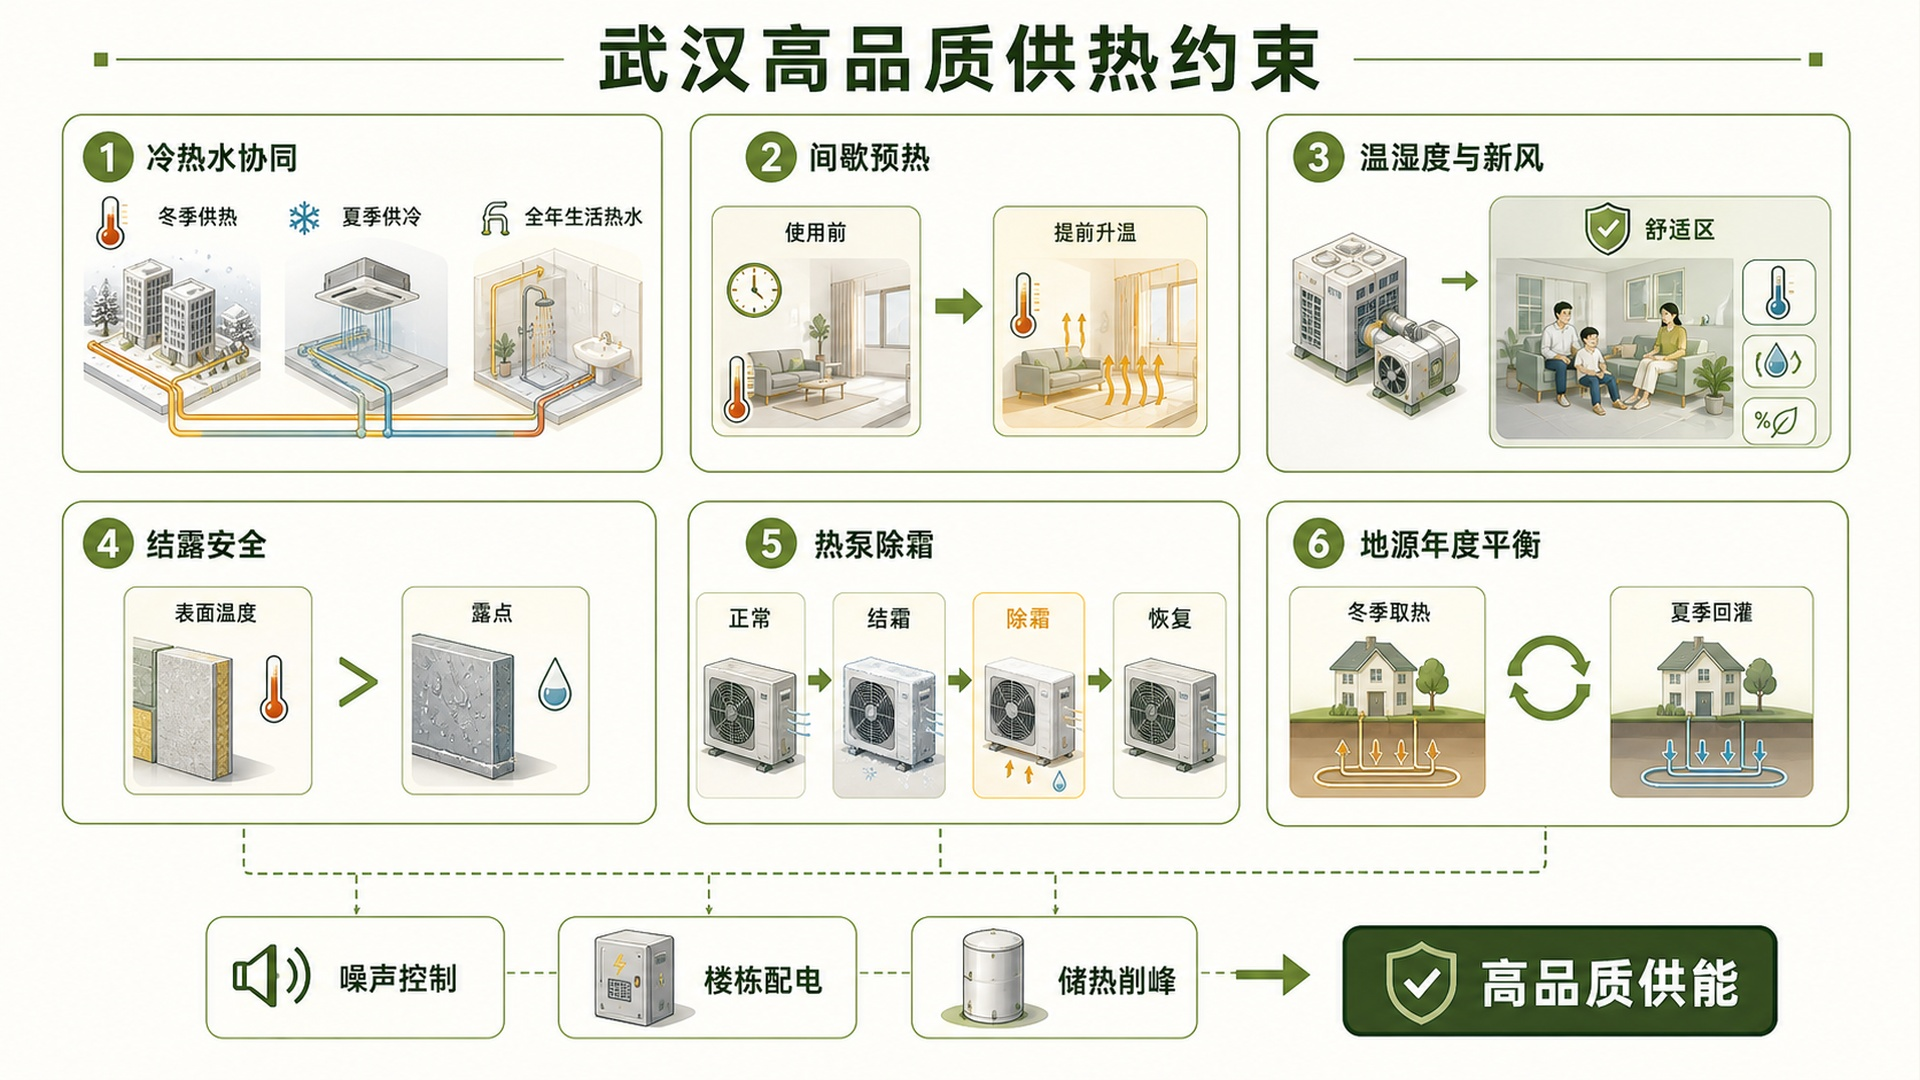
\includegraphics[width=0.76\textwidth,height=0.35\textheight,keepaspectratio]{media/model-cn/14_武汉高品质供热约束.jpg}
\caption{武汉供热约束}
\label{fig:model-cn-wuhan-quality}
\end{figure}

\subsection{场景差异}

三类场景共享负荷预测、能量平衡、容量演化、储热递推和舒适度约束，但规划对象和主导边界不同。乌鲁木齐侧重存量资产重构与极寒保供，固原侧重空间选址、燃料供应和微网可靠性，武汉侧重系统形态与多服务品质。共核与差异关系见图\ref{fig:model-cn-adapters}。

\begin{figure}[H]
\centering
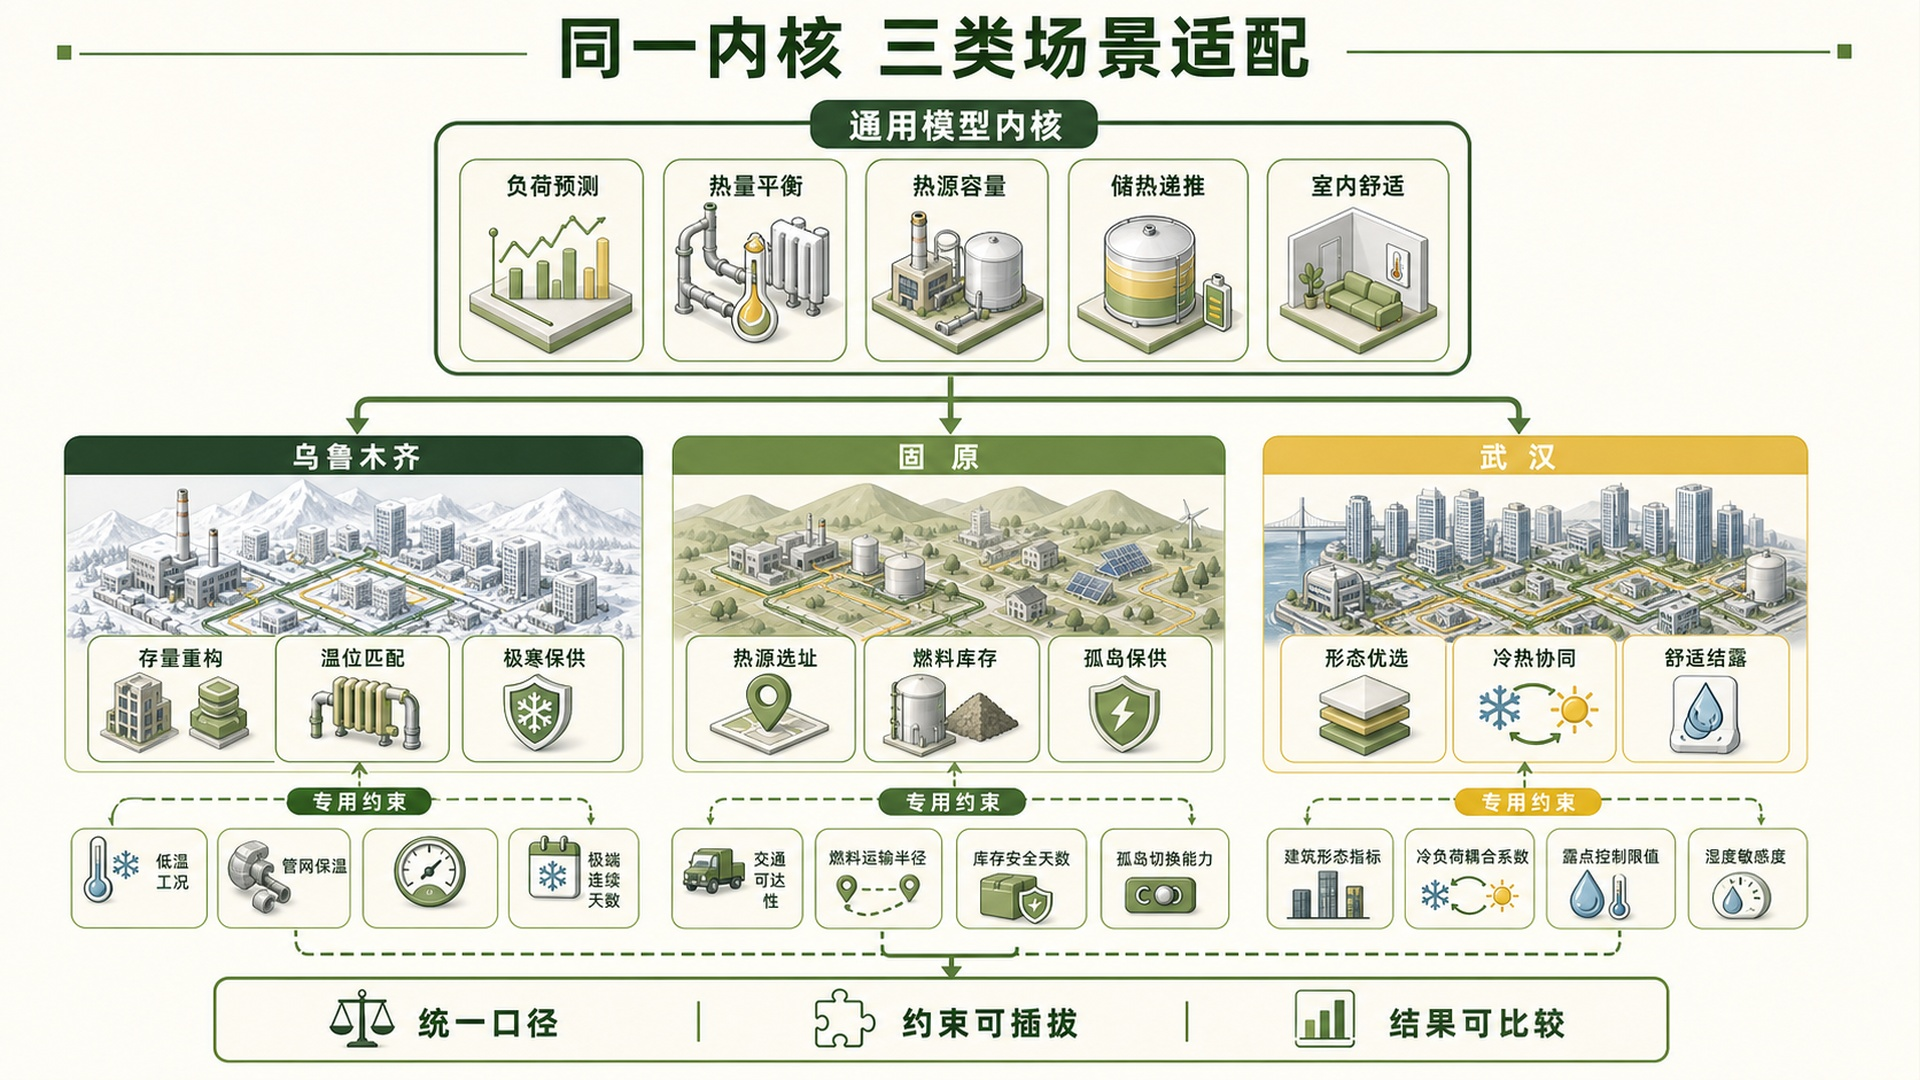
\includegraphics[width=0.76\textwidth,height=0.36\textheight,keepaspectratio]{media/model-cn/15_三城市共核异构.jpg}
\caption{三城市场景适配}
\label{fig:model-cn-adapters}
\end{figure}

\begin{table}[H]
\centering
\caption{三类场景的模型差异}
\small
\begin{tabularx}{\textwidth}{@{}p{0.13\textwidth}XXX@{}}
\toprule
维度 & 乌鲁木齐 & 固原 & 武汉\\
\midrule
初始条件 & 既有热源、骨干网和换热站 & 管网覆盖不足、分散热源较多 & 无传统集中供热资产\\
主要决策 & 热源退役、余热接入、管网降温 & 选址、用户分配、微网与燃料供应 & 供热形态、冷热水协同与配电\\
主导约束 & 温位、骨干网、N-1与寒潮保供 & 服务半径、库存、孤岛与防冻结 & 舒适、新风、结露、除霜与噪声\\
校核重点 & 远端温度、流量和回水温度 & 燃料到货、连通性和关键用户 & 温度恢复、地源平衡和配电容量\\
\bottomrule
\end{tabularx}
\end{table}

\subsection{统一校核}

三类场景采用相同的基础验收判据：逐时热量平衡残差不超过$\varepsilon_Q$，储热状态残差不超过$\varepsilon_E$，管网流量利用率不超过1，购电功率不超过接入容量，正常工况和规定压力情景下失供率为0。温度类判据按模型对象分别适用：启用楼栋级室温递推的算例验收绝对室温是否位于舒适区间；三个主算例的主链采用聚合等效热状态，其验收对象是该状态的最大温度偏移、逐时恢复损失率与舒适偏差惩罚，不表述为绝对室温达标。统一指标与场景专用指标的对应关系见图\ref{fig:model-cn-acceptance}。

\begin{figure}[H]
\centering
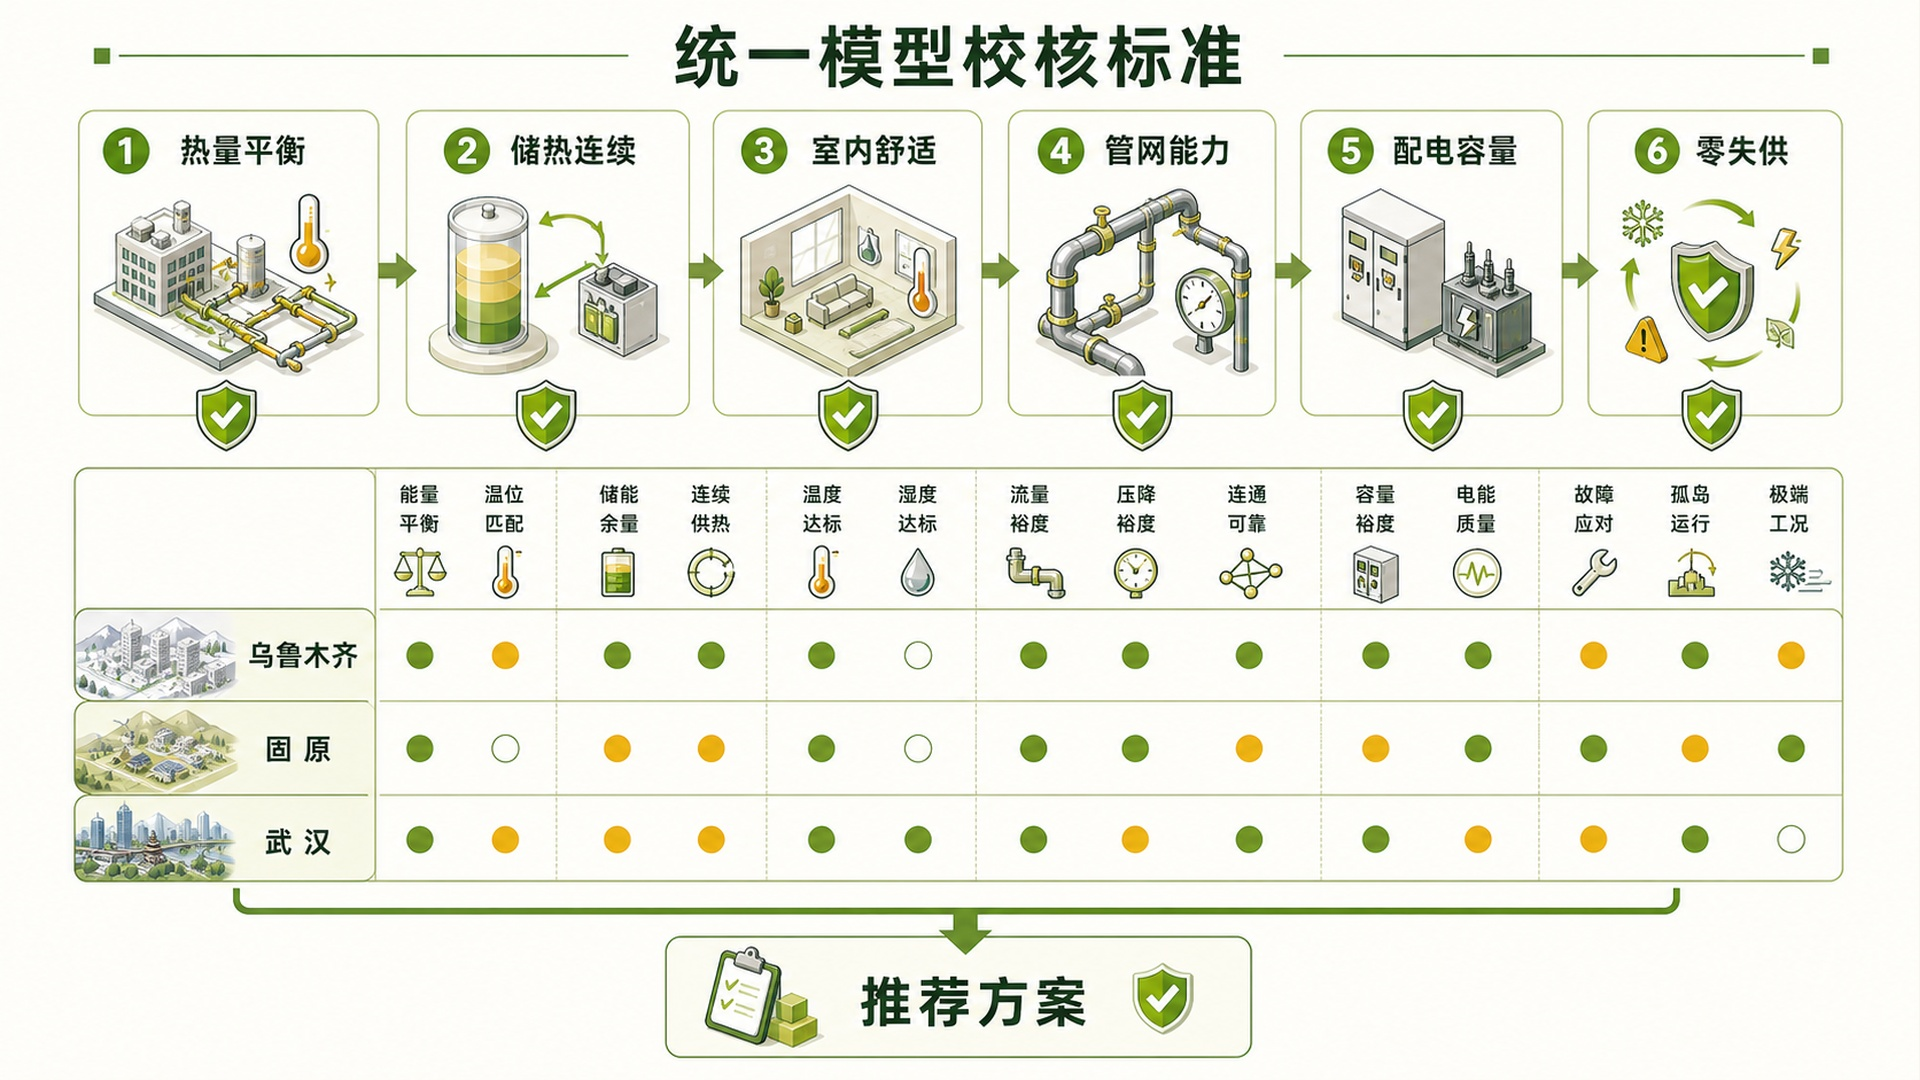
\includegraphics[width=0.76\textwidth,height=0.36\textheight,keepaspectratio]{media/model-cn/16_统一模型校核标准.jpg}
\caption{统一模型校核指标}
\label{fig:model-cn-acceptance}
\end{figure}

上述模型为后续算法提供变量、目标函数和可行域。规划变量确定资产与容量，运行变量描述供暖季逐时状态，工程校核用于确认候选方案满足连续物理边界。


\clearpage
\section{多场景多尺度源荷协同优化方法}

本节构建多目标协同求解方法，描述城市、区域和用户三个尺度的耦合关系，并从收敛性、计算效率和边界扰动等方面检验求解结果。

\subsection{方法框架与可复现性}

算法输入包括逐时气象、分时电价、设备与财务参数、城市热网和建筑群画像；输出包括投资方案与逐时调度方案。投资变量涉及设备容量、温位模式、候选管径、储热规模、配电增容和用户侧改造，运行变量包括各热源出力、管网流量与温位、储热状态、需求响应量等。评价指标覆盖成本构成、碳排放、失供量、舒适度偏差和火用损失。

模型采用1~h时间步长。2024---2025供暖季中，乌鲁木齐取[2024-10-10, 2025-04-11)的法定供热期，固原取[2024-10-15, 2025-04-16)的法定供热期，武汉取[2024-11-16, 2025-03-16)的项目服务周期；连续计算时长分别为4392~h、4392~h和2880~h，时间区间采用左闭右开形式。固原窗口依据《固原市城市供热管理办法》（固原市人民政府令第3号，2024年10月19日施行）第十三条的常规采暖供热期；该市2024---2025年度采暖费缴纳通知按当年实际计费期166天（3984~h）执行，属通知所列计费期，与本文模拟窗口分列。武汉不属于国家强制集中供暖区，其窗口只能表述为项目服务周期，不表述为全市法定供暖季。每次求解均记录配置、输入数据指纹、求解状态和相对间隙，以形成可核验的计算记录。算法总体流程如图\ref{fig:alg-overview}所示。

\begin{figure}[H]
\centering
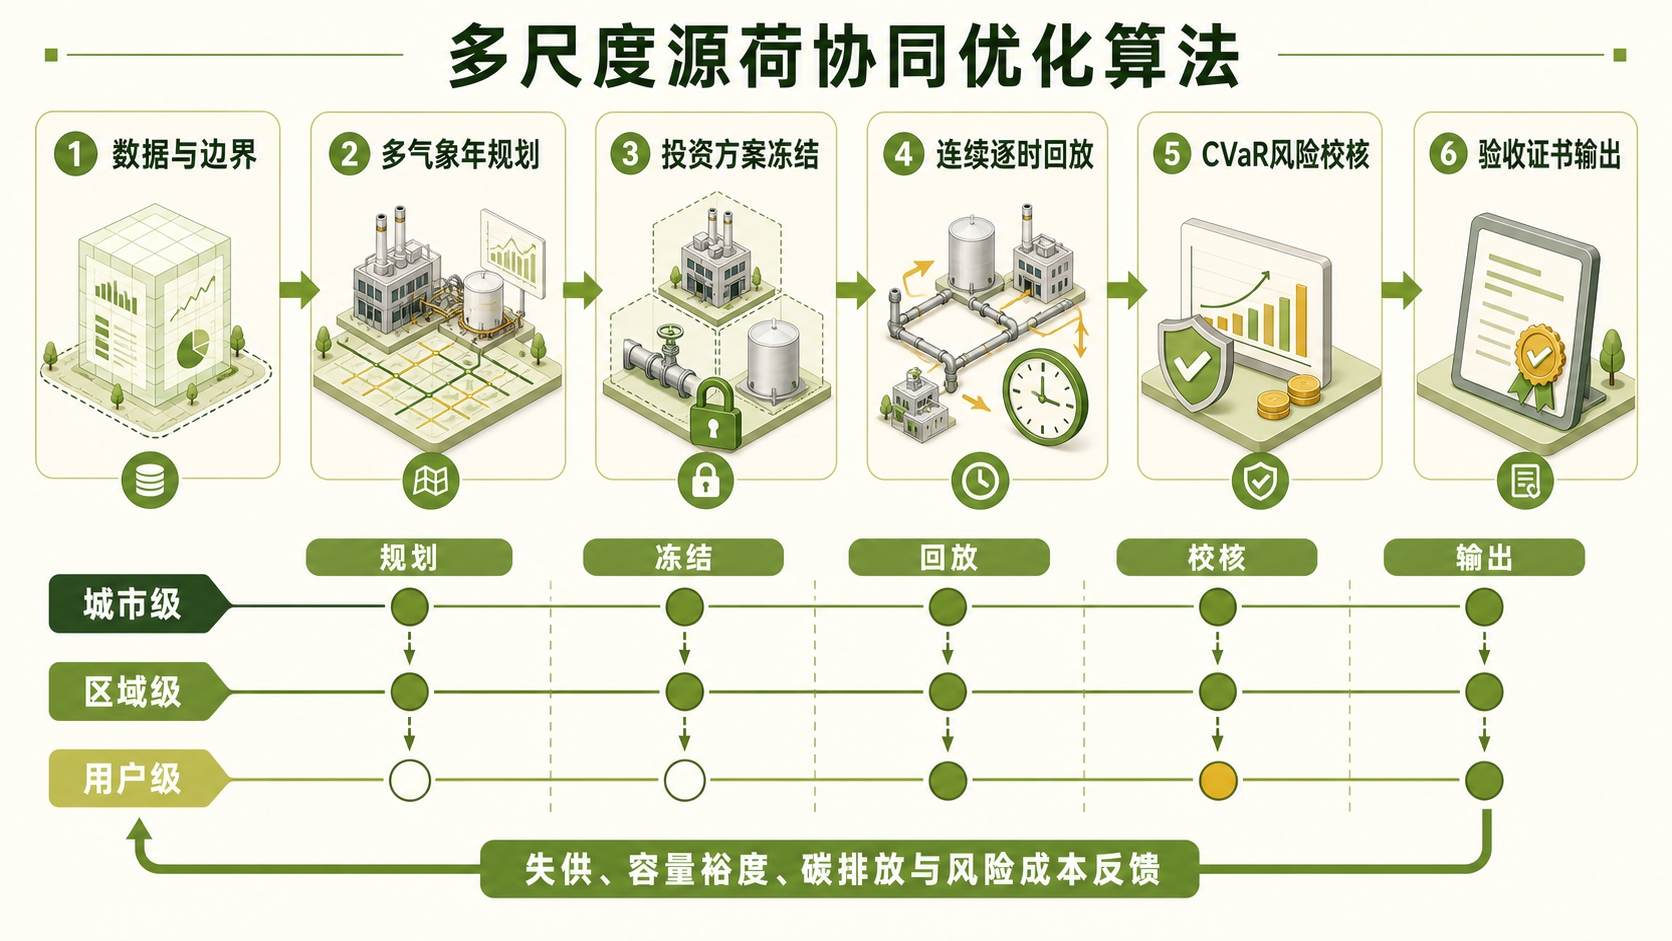
\includegraphics[width=0.76\textwidth,height=0.38\textheight,keepaspectratio]{media/algorithm-revision/fig1.png}
\caption{多尺度源荷协同优化算法总体流程}
\label{fig:alg-overview}
\end{figure}

与确定性单情景规划及工程手册式方案比选相比，本文算法的主要差异见表\ref{tab:alg-comparison}。

\begin{table}[H]
\centering
\caption{常见做法与本文算法的对照}
\label{tab:alg-comparison}
\begin{tabularx}{\textwidth}{p{0.27\textwidth}p{0.35\textwidth}X}
\toprule
常见做法 & 本文算法 & 核验依据\\
\midrule
逐时离散化、确定性单情景规划 & 1~h全季求解，并开展多情景与极端年全年回放 & 主解求解记录、极端年累计61392~h回放\\
采用规划手册指标评价方案 & 单一MILP主解，并进行$\varepsilon$-约束与风险扫描 & 求解状态、上下界和相对间隙\\
规划与运行分开处理 & 三场景同一条管线：代表时段投资---运行联合规划，再冻结投资完成全季运行校核 & 规划层与回放层分别记录状态和间隙\\
\bottomrule
\end{tabularx}
\end{table}

\subsection{多尺度模型}

模型由城市层、区域层和用户层构成，各层通过共享投资变量、逐时运行变量和状态耦合约束连接。三个算例均采用3个聚合负荷节点；乌鲁木齐、固原和武汉分别包含7、6、7类热源和3、2、1条聚合管段。城市层对应总体投资与技术路线，区域层对应热源和输配单元，用户层对应同类建筑负荷的聚合节点。其关系如图\ref{fig:alg-multiscale}所示。

\begin{figure}[H]
\centering
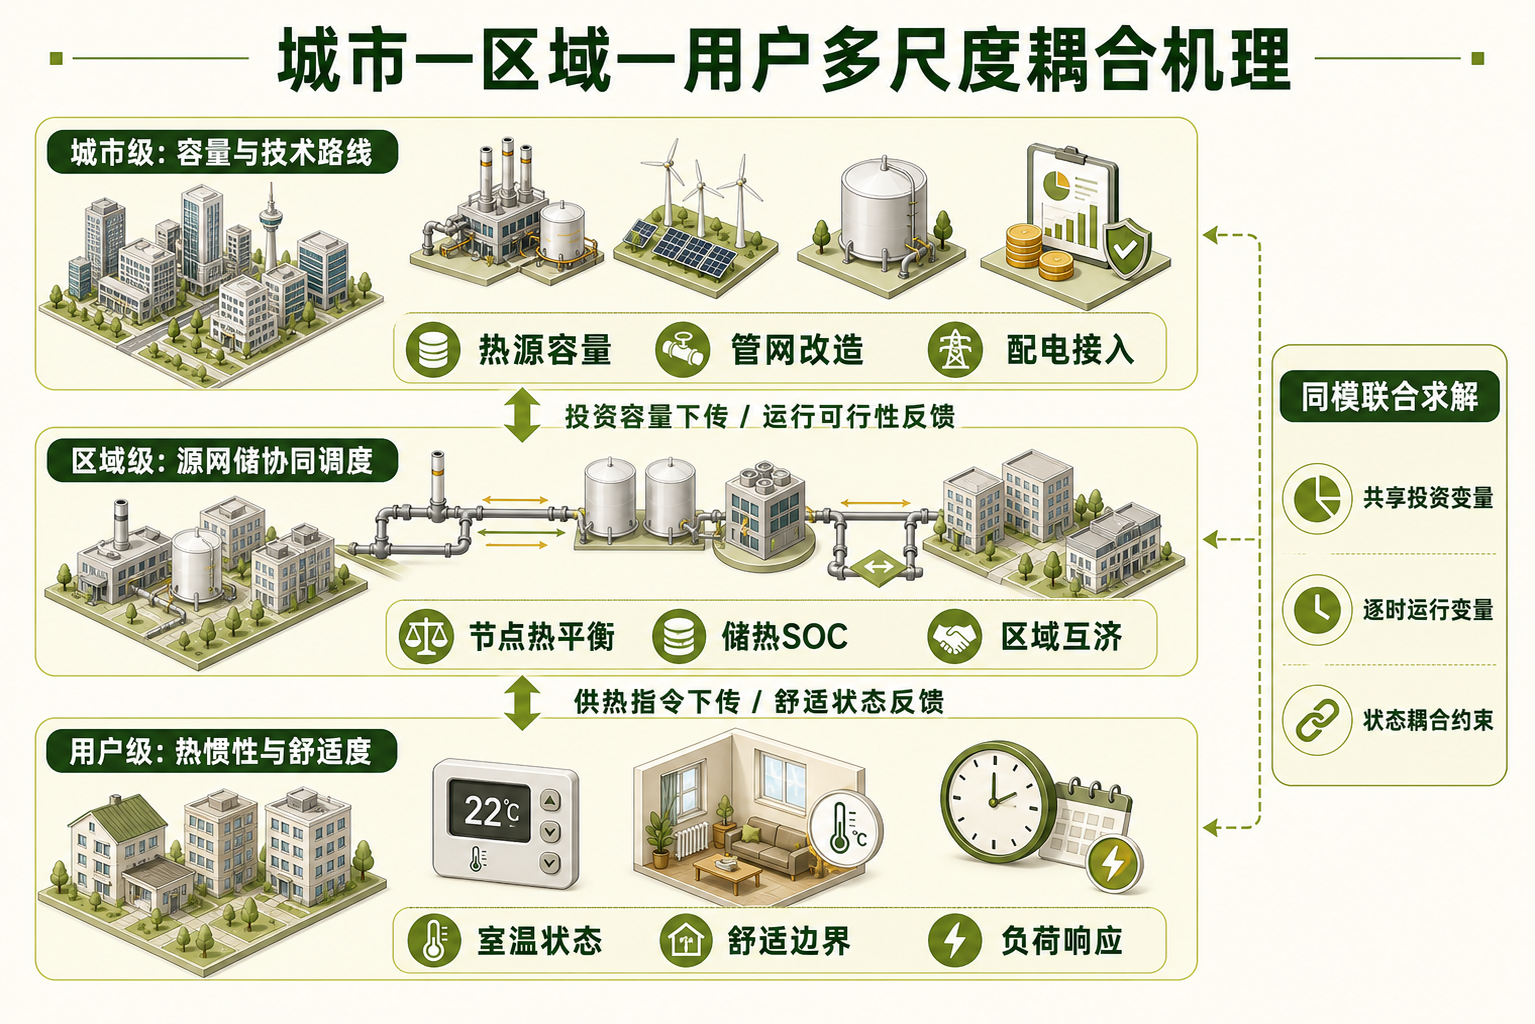
\includegraphics[width=0.76\textwidth,height=0.30\textheight,keepaspectratio]{media/algorithm-revision/fig2.png}
\caption{城市---区域---用户多尺度耦合机制}
\label{fig:alg-multiscale}
\end{figure}

城市层确定容量与技术路线，包括新增或退役机组容量、热源温位模式、候选管径、储热规模以及配电接入和增容。候选技术链依据资源、场地、配电和政策条件生成并预筛，本次计算执行容量、拓扑和温级预审。

区域层描述能流、管网与储热。模型在节点和75/45~$^{\circ}$C两级温位上建立逐时能量平衡。温位兼容约束阻止低温热源直接供应高温需求，高温热源供应低温需求时将品位损失计入火用失配惩罚：
\begin{equation}
T_{\mathrm{src}}^{\min}\geq T_{\mathrm{sup}}+\Delta T_{\mathrm{he}},
\label{eq:alg-grade}
\end{equation}
其中，$T_{\mathrm{src}}^{\min}$为热源供水温度下界，$T_{\mathrm{sup}}$为用户供水温度要求，$\Delta T_{\mathrm{he}}$为换热端差。管网采用温位线性化和双向流动互斥约束，储热状态按下式递推：
\begin{equation}
E_{s,t}=(1-\mu_s)E_{s,t-1}+\eta_{\mathrm{ch}}q_{s,t}^{\mathrm{ch}}\Delta t-\frac{q_{s,t}^{\mathrm{dis}}\Delta t}{\eta_{\mathrm{dis}}},
\label{eq:alg-storage}
\end{equation}
其中，$\mu_s$为自损失率，$\eta_{\mathrm{ch}}$和$\eta_{\mathrm{dis}}$分别为充、放热效率。

用户层描述聚合节点的热惯性与负荷调节。状态上下界、需求响应窗口守恒和参与率上限共同约束用户侧调节行为。凡启用楼栋级室温递推的算例，其室温按一时段内热输入不变条件下的精确离散递推：
\begin{align}
a_n&=\exp\!\left(-H_n\Delta t/C_n\right),\qquad \beta_n=\frac{1-a_n}{H_n},\\
\theta_{n,t}&=a_n\theta_{n,t-1}+(1-a_n)T_t^{\mathrm{out}}
+\beta_n\!\left(Q_{n,t}^{\mathrm h}-Q_{n,t}^{\mathrm c}+G_{n,t}\right),
\label{eq:alg-building}
\end{align}
其中，$\theta_{n,t}$为时段末室温，$C_n$为等效热容，$H_n$为围护与通风合并的总传热系数，$G_{n,t}$为内部与太阳得热之和。该式是时段内输入不变时的精确积分，不是差分近似。本条与式\eqref{eq:load-decomp}后的聚合等效蓄热描述的是两套不同对象：三场景主链采用聚合等效热状态，楼栋级室温用于启用该模块的算例并单独登记初末温度，两者不互相替代，也不共用初末边界。

三个尺度通过容量、温位和建筑改造三类连接相互约束：容量约束将运行出力限制在可用率及设备上下限内；温位匹配表完成“源温---网温---节点负荷”匹配；用户侧调节量先进入节点热平衡，再由热源出力与储热充放共同响应。例如在已有逐时结果中，用户侧负荷削减使同一时段节点需求下降，优先减少边际热源出力；恢复负荷出现时，储热先放热并由可调热源补足剩余需求，节点平衡在每个时段保持闭合。三个场景采用同一条求解管线：先在代表时段上完成投资---运行联合规划，再冻结投资方案进行完整时序运行校核；规划层与回放层分别报告求解状态与相对间隙。因此，推荐方案用于工程可行性比较，不将代表时段投资层的结果表述为全季最优。

\subsection{多目标协同优化}

成本与碳排放采用$\varepsilon$-约束法协调，而不直接将不同量纲的成本和碳排放加权相加。模型以全生命周期净成本的等年值最小为目标，同时设置碳排放上限；逐档收紧上限并重新求解完整供暖季，相邻两档的成本增量与减排量之比用于计算边际减排成本。

乌鲁木齐场景中，成本端点为27.49万元、27.32~t~CO$_2$，排放端点为74.81万元、10.57~t~CO$_2$。本文推荐记录采用通过全部硬约束与工程检查的方案，等年值成本为27.76万元、碳排放为27.31~t~CO$_2$；该记录与仅按目标函数排序得到的成本端点分开标注。单位供热成本由基准方案的0.078851元/kWh增至0.100681元/kWh，增加27.69\%。该增幅反映以成本增加换取减排、清洁热利用和可靠性约束的综合取舍。

零失供、清洁热比例、N$-1$容量裕度、地源年度平衡和舒适度上下限作为硬边界，不与经济性目标交换。失供率约束为
\begin{equation}
U_{\mathrm{un}}=\frac{\sum_t q_t^{\mathrm{un}}}{\sum_t Q_t}\leq U_{\max},
\label{eq:alg-unserved}
\end{equation}
其中，$q_t^{\mathrm{un}}$为失供功率，$Q_t$为热需求，$U_{\max}=0$表示推荐方案不允许失供。边界内的需求移峰和舒适偏差通过惩罚成本进行优化。

气象不确定性作为独立风险层，采用
\begin{equation}
\min\ \mathbb{E}[C]+\lambda\operatorname{CVaR}_{\alpha}(C),
\qquad \alpha=0.8,
\label{eq:alg-risk-objective}
\end{equation}
其中，$\lambda$取0、0.02、0.05和0.10四档。条件风险价值采用Rockafellar--Uryasev线性化：
\begin{equation}
\operatorname{CVaR}_{\alpha}(C)=\min_{\eta,z_s}\left\{\eta+\frac{1}{1-\alpha}\sum_s p_sz_s\right\},
\quad z_s\geq C_s-\eta,\quad z_s\geq0.
\label{eq:alg-cvar}
\end{equation}

$\lambda=0.05$作为三个场景的统一参考值。多气象年风险层中，乌鲁木齐的期望成本增加0.012万元、CVaR下降0.831万元；固原的期望成本增加0.016万元、CVaR下降0.515万元，变化约占年化成本的0.01\%。武汉场景的投资不随风险权重改变，说明其投资方案主要由硬约束决定。不同风险权重下的结构变化见表\ref{tab:alg-lambda}。

\begin{table}[H]
\centering
\caption{多气象年风险层的$\lambda$权重扫描结果}
\label{tab:alg-lambda}
\begin{tabularx}{\textwidth}{cXXX}
\toprule
$\lambda$ & 乌鲁木齐 & 固原 & 武汉\\
\midrule
0.02 & 余热源热泵、备用电锅炉和配电容量首次调整 & 投资配置不变 & 投资配置不变\\
0.05 & 继续小幅调整 & 储热与微网可再生增加，生物质调峰减少 & 投资配置不变\\
0.10 & 进一步转入风险平衡 & 与0.05档接近 & 投资配置不变\\
\bottomrule
\end{tabularx}
\end{table}

$\lambda$扫描来自2020---2024多气象年全年回放，用于风险机制专项验证；供暖季主结果中的成本---碳Pareto采用确定性单情景计算。风险层共包含12个规划案例（3个场景$\times$4档$\lambda$），全部收敛，60项年度容量审计通过，CVaR一致性核验误差为$5.59\times10^{-9}$元。图\ref{fig:alg-objectives}展示的是该专项风险层的12/12案例收敛与60/60容量审计结果，不等同于供暖季推荐方案的13道机器验收。

\begin{figure}[H]
\centering
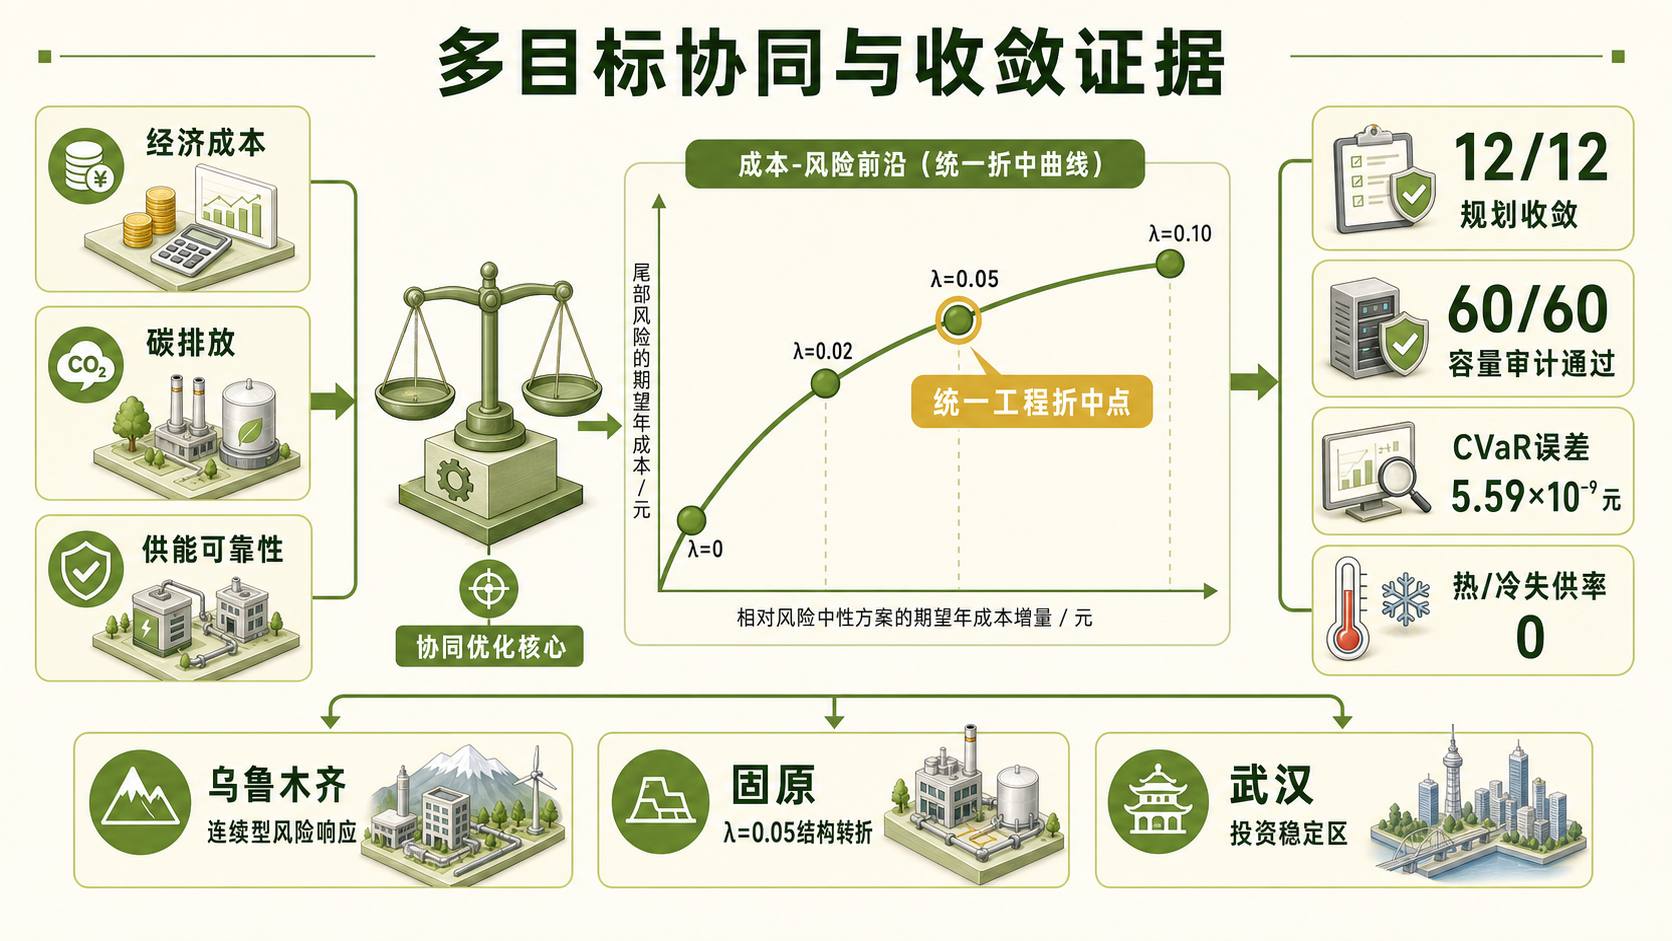
\includegraphics[width=0.76\textwidth,height=0.30\textheight,keepaspectratio]{media/algorithm-revision/fig3.png}
\caption{多目标协同与风险层收敛证据}
\label{fig:alg-objectives}
\end{figure}

\subsection{求解流程与收敛准则}

模型构造器采用Python~3.11实现，并通过SciPy的\texttt{milp}接口调用HiGHS求解。约束矩阵按CSR/CSC稀疏格式编译和缓存，模型装配约需1.6~s，未使用自定义割。机组启停采用凸包重建模，开机状态保留为二元变量，启动和停机辅助变量连续化。全年回放单城测试中，整数变量数量由26280个减至8760个。

求解流程包括四步：首先完成配置与指标初始化；其次进行候选技术链预筛；然后按$\varepsilon$-约束或风险权重批量求解；最后进行逐时回放和验收审计。收敛需同时满足以下条件：求解状态达到全局最优或允许间隙并具有上下界证明；可行解与对偶界形成可解释的相对MIP gap；约束残差不超过$10^{-6}$；逐时回放与后验复核通过。

表\ref{tab:alg-solver}登记三个场景代表时段规划阶段的求解记录。该组数值为初赛轮次的实验记录：代表时段规划层相对间隙分别为$1.53\times10^{-4}$、$1.84\times10^{-3}$和0.98\%，逐时热平衡最大绝对残差依次为$7.41\times10^{-13}$、$1.25\times10^{-10}$和$8.53\times10^{-14}$~kW。该组记录未随附可回查的求解日志，本稿以历史报告值列出，逐行核验状态见表中「来源状态」列；本次补充验证可回查的同类记录见表\ref{tab:alg-supplement}。

\begin{table}[H]
\centering
\caption{三场景代表时段规划求解记录（历史报告值）}
\label{tab:alg-solver}
\small
\begin{tabularx}{\textwidth}{@{}p{0.07\textwidth}p{0.13\textwidth}p{0.12\textwidth}p{0.08\textwidth}p{0.12\textwidth}p{0.17\textwidth}X@{}}
\toprule
场景 & 求解方法 & 整数变量 & 时间/s & 相对间隙 & 来源状态 & 验收\\
\midrule
乌鲁木齐 & 代表时段投资---运行联合规划 & 启停二元8784个 & 531.1 & $1.53\times10^{-4}$ & 初赛记录，无日志 & 原稿记载通过（未核验）\\
固原 & 代表时段投资---运行联合规划 & 启停二元4392个 & 64.0 & $1.84\times10^{-3}$ & 初赛记录，无日志 & 原稿记载通过（未核验）\\
武汉 & 代表时段投资---运行联合规划 & 0 & 31.7 & 0.98\% & 初赛记录，无日志 & 原稿记载通过（未核验）\\
\bottomrule
\end{tabularx}
\end{table}

表\ref{tab:alg-supplement}为本次修订实际执行并留存的补充验证。三个场景在同一套来源锁定的公开输入上，按“代表时段规划---冻结投资---可靠容量审计---全年连续回放”顺序求解；求解状态、可行目标值、求解下界、相对间隙、耗时、逐时残差与违约小时均取自落盘的运行记录。

\begin{table}[H]
\centering
\caption{补充验证：三场景冻结投资全年回放求解与验收登记}
\label{tab:alg-supplement}
\small
\begin{tabularx}{\textwidth}{@{}p{0.07\textwidth}p{0.05\textwidth}p{0.055\textwidth}p{0.135\textwidth}p{0.085\textwidth}p{0.115\textwidth}p{0.085\textwidth}p{0.055\textwidth}X@{}}
\toprule
场景 & 阶段 & 终止状态 & 可行值 / 下界（万元） & 相对间隙 & 最大约束违反量 & 耗时/s & 失供率 & 验收项\\
\midrule
乌鲁木齐 & 规划 & 0 & 65.788 / 65.661 & $1.93\times10^{-3}$ & $5.190\times10^{-11}$ & 0.94 & 0 & ---\\
乌鲁木齐 & 回放 & 0 & 66.065 / 66.012 & $8.13\times10^{-4}$ & $9.963\times10^{-7}$ & 49.46 & 0 & 15/15\\
固原 & 规划 & 0 & 135.774 / 135.770 & $3.17\times10^{-5}$ & $6.253\times10^{-13}$ & 14.87 & 0 & ---\\
固原 & 回放 & 0 & 138.057 / 137.410 & $4.69\times10^{-3}$ & $9.997\times10^{-7}$ & 32.60 & 0 & 16/16\\
武汉 & 规划 & 0 & 54.603 / 54.603 & 0 & $8.188\times10^{-13}$ & 0.80 & 0 & ---\\
武汉 & 回放 & 0 & 56.029 / 56.029 & 0 & $8.837\times10^{-7}$ & 74.28 & 0 & 17/17\\
\bottomrule
\end{tabularx}
\end{table}

\noindent{\footnotesize 注：「终止状态」列为求解器返回状态，0 表示按登记的绝对容差 $10^{-6}$、相对容差 $10^{-8}$ 与相对间隙阈值判定最优；相对间隙非零的行，其最优性在该登记容差内成立。「最大约束违反量」取该阶段数值审计的最大约束违反量，单位为对应约束自身的单位。储热状态方程最大残差与各储热装置的初末状态另见同包交付的《仿真结果数据表》。}

该组回放覆盖2023年完整日历年8760~h，时间步长1~h，验证同一模型与配置在完整年时间轴上的连续性与可靠性；主结果供暖季窗口的登记与核验状态见表\ref{tab:alg-solver}的「来源状态」列。武汉的两阶段求解在补齐代表时段锚点后通过全部验收项；未补齐时其冻结投资方案因并网可靠电力容量低于全年需求$0.1058$~kW而被就绪审计拒绝，该锚点修正与新旧容量对照登记于同包交付的《仿真结果数据表》。

敏感性测试的20档扰动获得有效解，其中乌鲁木齐电价高档和余热低档为时间受限近似解，相对间隙分别为7.05\%和9.44\%；另有固原负荷低档、武汉碳价高档两档未收敛。乌鲁木齐Pareto中间档的部分点在时限内间隙为13.2\%---13.7\%。固原三档采用推荐投资模式复算，全部满足碳排放上限，间隙为0.20\%、0.22\%和0.24\%，这些结果属于冻结投资模式的运行参考点，不代表完整联合MILP重新寻优。

为检验乌鲁木齐排放端点投资模式在不同碳帽下的运行可达性，固定排放最优解的投资、退役、管径、储热和末端改造模式，对23365、19136和14906~kg三档碳帽进行全季运行重算。三档实际排放均为10616.5~kg，失供率为0，求解状态均为Optimal，相对间隙为$1.90\times10^{-7}$。运行成本为11.271万元/年，仅包含运行费用，不与联合解中包含资本成本的Pareto结果直接比较。

\subsection{计算效率与扩展性}

求解效率的改善主要来自启停凸包重建模和稀疏编译缓存。固原全年回放用时由575.746~s降至86.903~s，提升6.63倍；两年度合计用时由602.483~s降至112.750~s，减少81.29\%。该结果来自多气象年全年回放的单城效率测试。单次供暖季问题约包含31万---45万个变量，乌鲁木齐场景的启停二元变量为8784个。连续温位、C\&CG、Benders分解和在线MPC作为可选扩展，本次计算未启用。逐时回放、边界检验和求解加速关系如图\ref{fig:alg-replay}所示。

\begin{figure}[H]
\centering
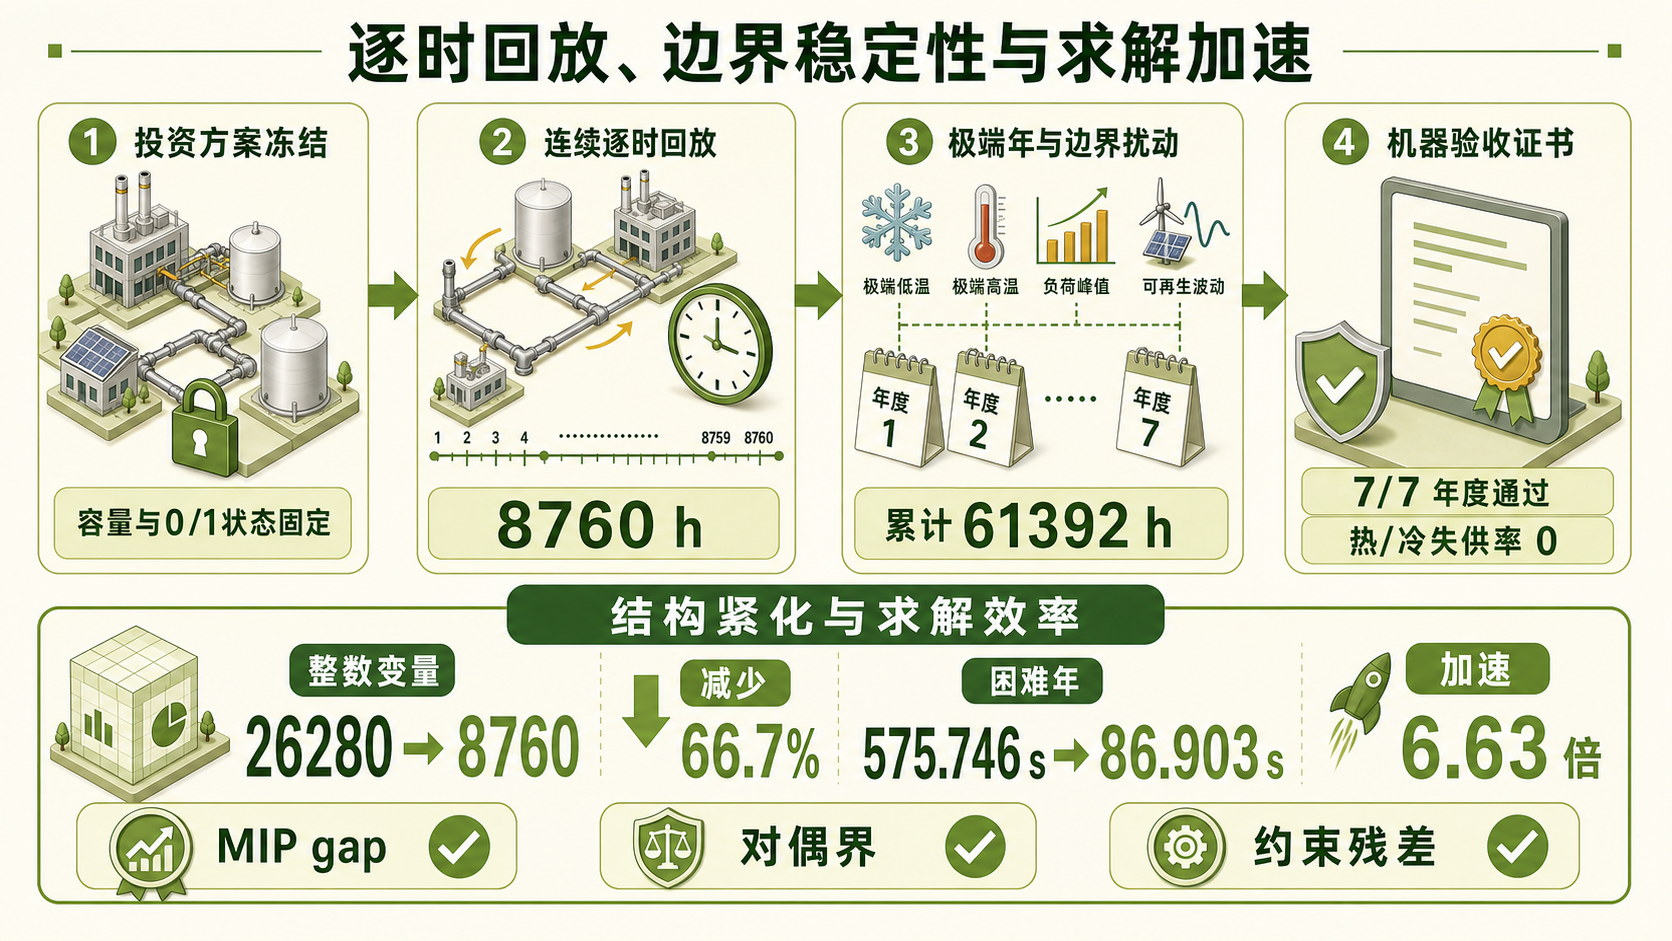
\includegraphics[width=0.76\textwidth,height=0.30\textheight,keepaspectratio]{media/algorithm-revision/fig4.png}
\caption{逐时回放、边界稳定性与求解效率}
\label{fig:alg-replay}
\end{figure}

\subsection{数值结果与敏感性}

图\ref{fig:code-kpi}比较了基准方案与推荐方案的成本、碳排放、清洁热利用和供热可靠性指标。推荐方案的取舍由成本、排放上限、清洁热占比和供热约束共同决定，因此各项指标的变化方向并不完全一致。图中成本采用年化等效值，单位供热成本按交付热量折算，二者与供暖季现金运行成本分别核算。

\begin{figure}[H]
\centering
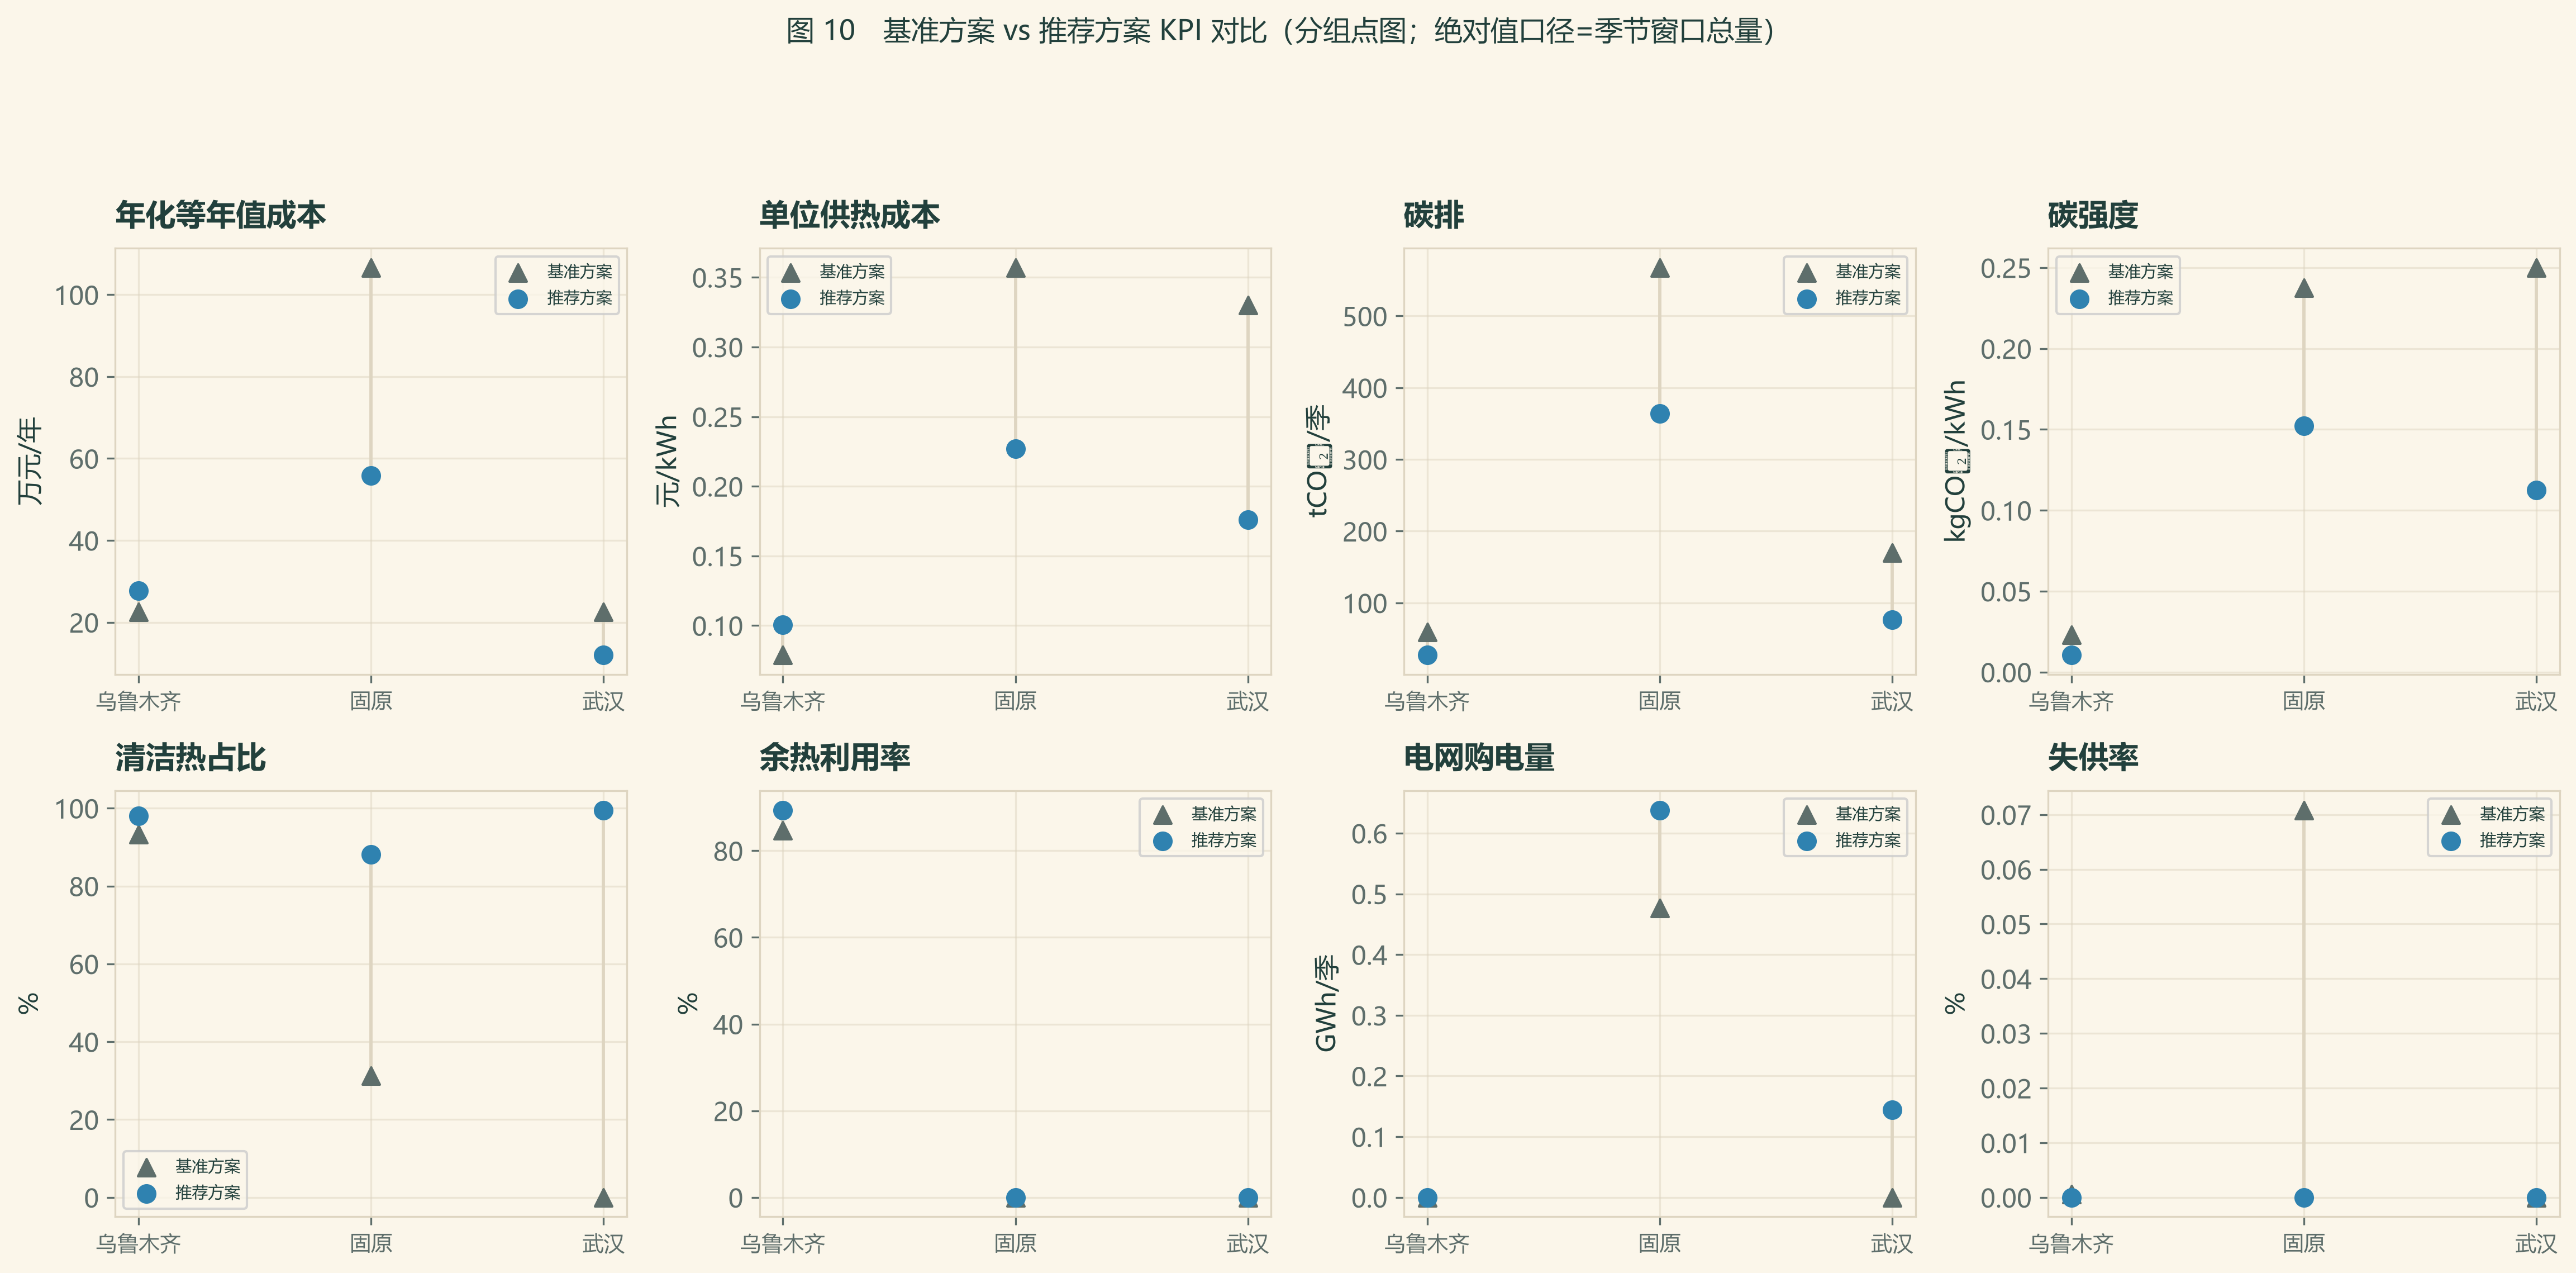
\includegraphics[width=0.98\textwidth,height=0.52\textheight,keepaspectratio,trim=0 0 0 100,clip]{media/code-results/fig10_kpi_comparison.png}
\caption{基准方案与推荐方案KPI对比}
\label{fig:code-kpi}
\end{figure}

成本与碳排放的候选解分布见图\ref{fig:code-pareto}。推荐方案从满足排放、可靠性和投资边界的候选解中选取，不必与最低成本点或最低排放点重合。部分点为固定投资模式下的运行参考点或时限内近似解，其求解状态和相对间隙以前文说明为准。

\begin{figure}[H]
\centering
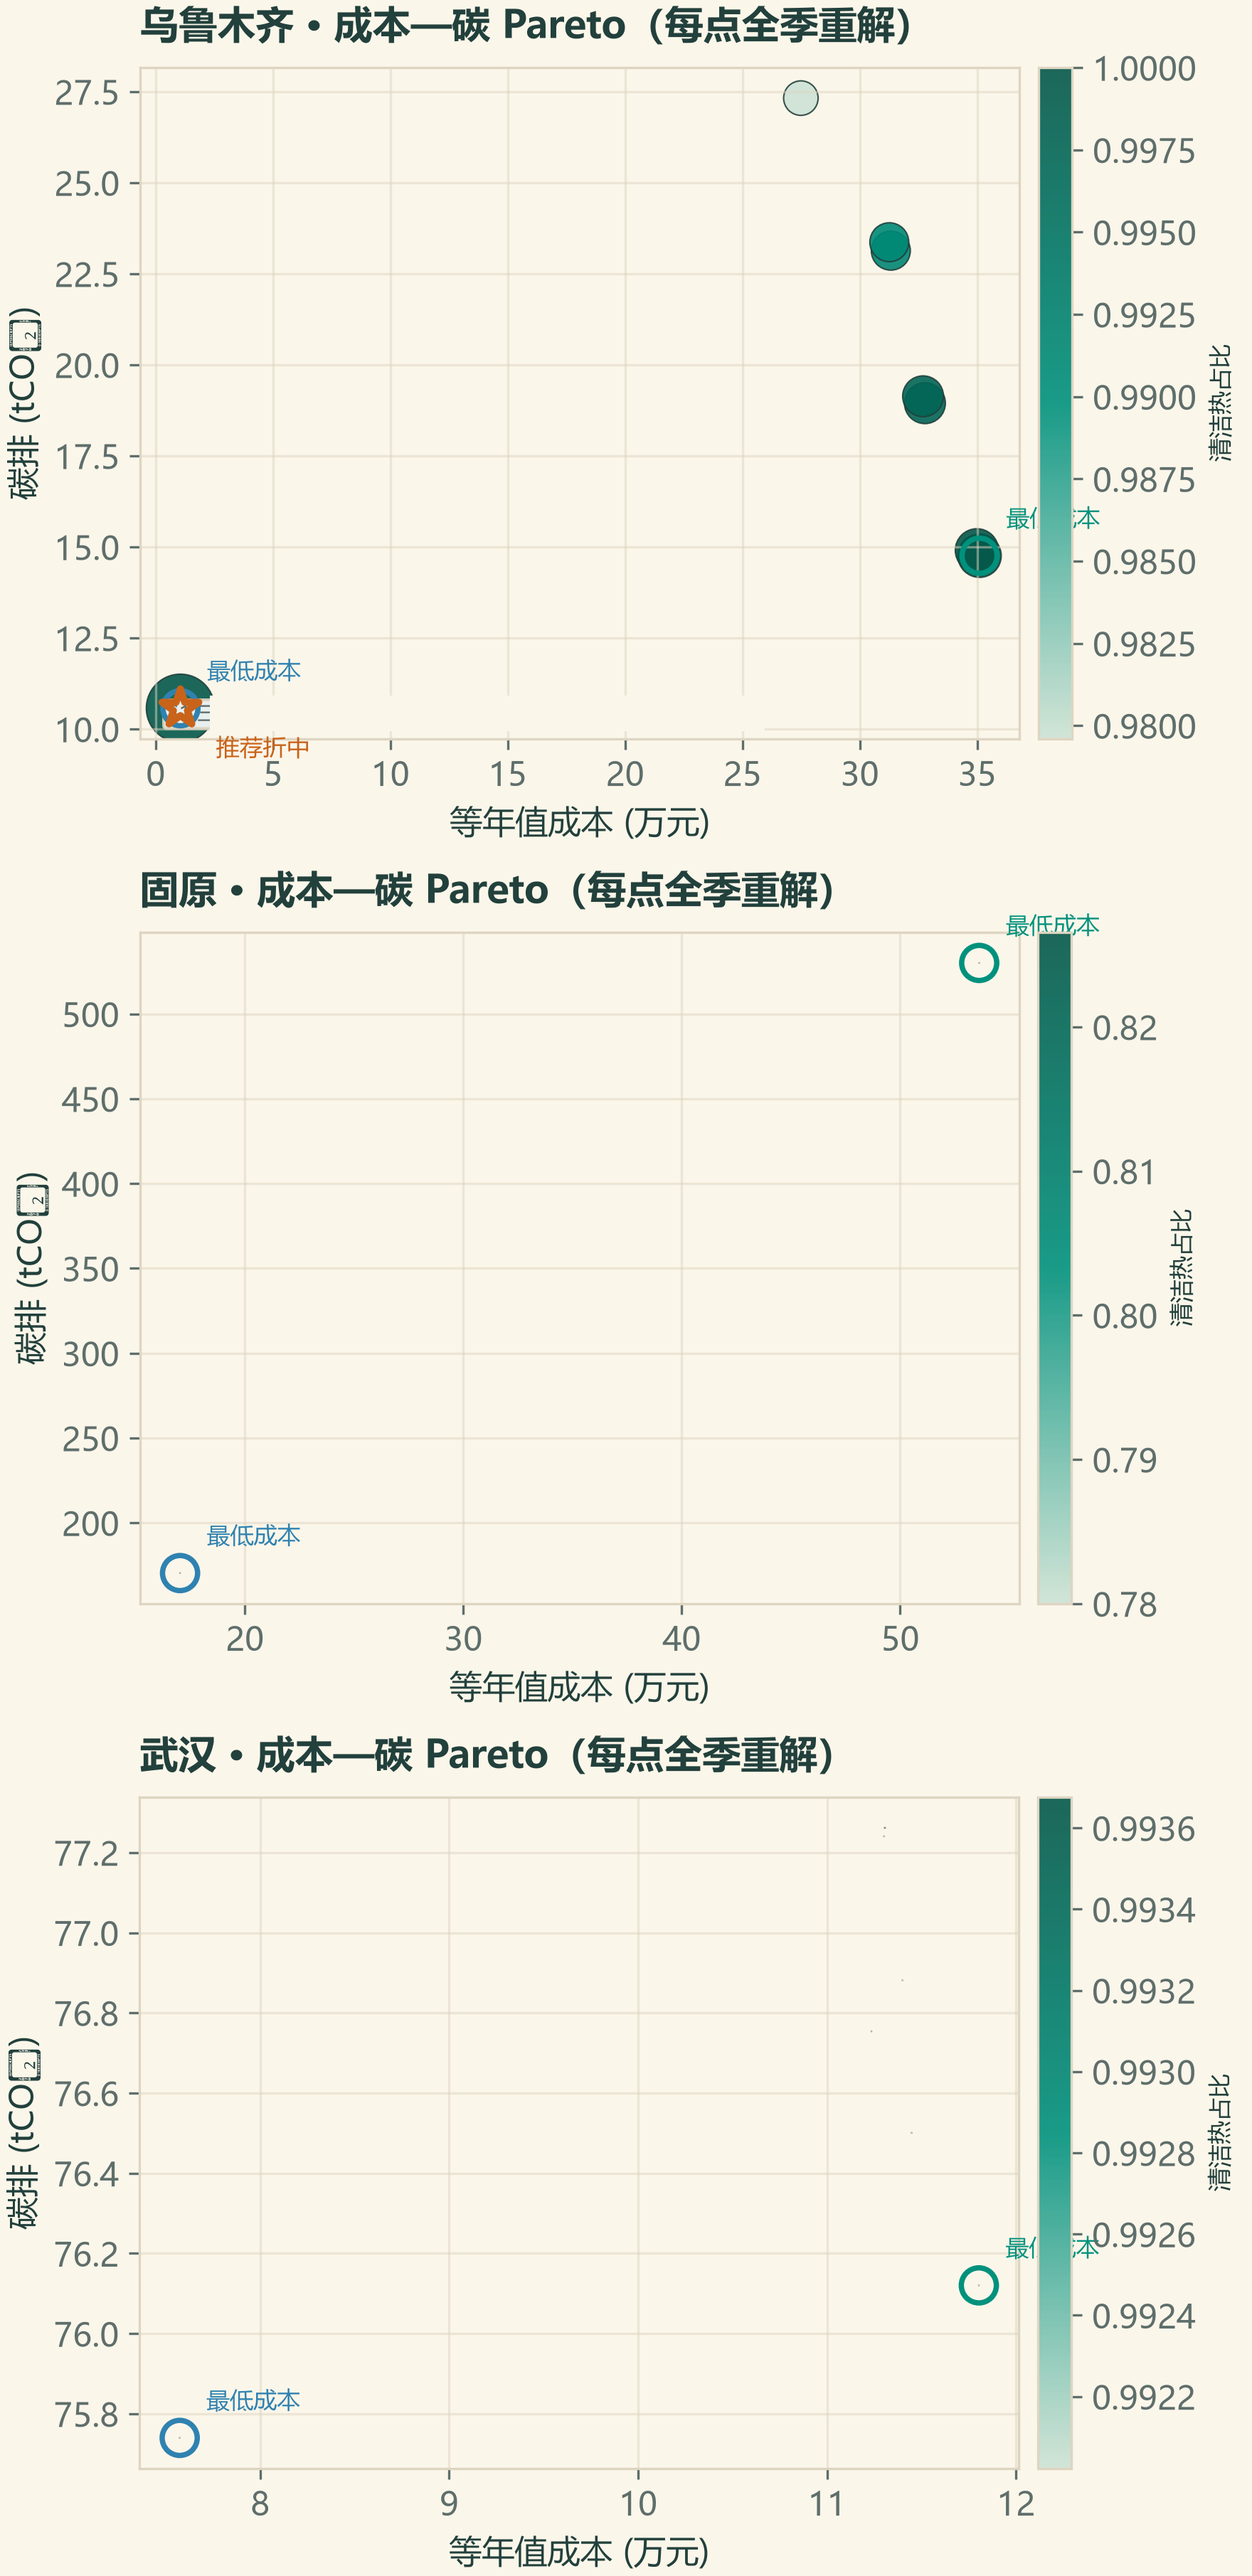
\includegraphics[width=0.82\textwidth,height=0.82\textheight,keepaspectratio]{media/code-results/fig11_cost_emission_pareto_stack.png}
\caption{三城市成本—碳排放候选方案对比（气泡大小为年化新增投资；乌鲁木齐面板左下重叠的三个标记分别为最低成本、推荐折中与同一位置上的时限内可行解，其中时限可行解的相对间隙为 13.2\%---13.7\%，最优性未证明）}
\label{fig:code-pareto}
\end{figure}

V4全年单情景消融实验沿用原时间权重，并在每次移除模块后重新求解投资与运行。完整模型的年化目标为95.620万元，碳排放为30.602万kg~CO$_2$。去掉需求响应后，年化成本增加0.09\%，购电量增加0.21\%；去掉新增储热后，年化成本增加3.55\%，碳排放增加6.05\%，购电量增加3.41\%；去掉火用失配惩罚后，火用损失增加4.90\%。该组结果用于检验V4模块贡献，与三城市供暖季推荐方案分开报告。

复合寒潮压力测试沿用V4算例，将室外温度序列整体降低8~$^{\circ}$C、负荷提高15\%、余热可用量降低15\%，并冻结投资变量。测试结果仍保持零失供；既有实验记录报告\textbf{运行目标值}增加18.55\%，购电量增加56.78\%，碳排放增加113.95\%。运行目标值含年化投资、碳成本、启停、运维与惩罚项，与能源现金支出分别核算，两者不可互相换算；该记录未随附可回查日志。逐档敏感性分析表明：乌鲁木齐对热负荷最敏感，成本变化为$+19.1\%/-17.9\%$，其次为余热下降和电价上升；固原的生物质到货扰动因库存缓冲未改变成本；武汉对电价和热负荷较敏感，变化范围分别为$+16.9\%/-14.6\%$和$+16.8\%/-13.7\%$。

最冷连续168~h的热源出力、负荷和储热状态见图\ref{fig:code-cold168}，用于检查低温持续期间的逐时供需平衡。图\ref{fig:code-worst72}进一步列出最不利72~h窗口内的可用供热能力、负荷、储热与容量裕度。两图分别反映常规极寒时段调度和压力场景下的边界状态，不据此假定三城市具有相同的储热运行模式。

\begin{figure}[H]
\centering
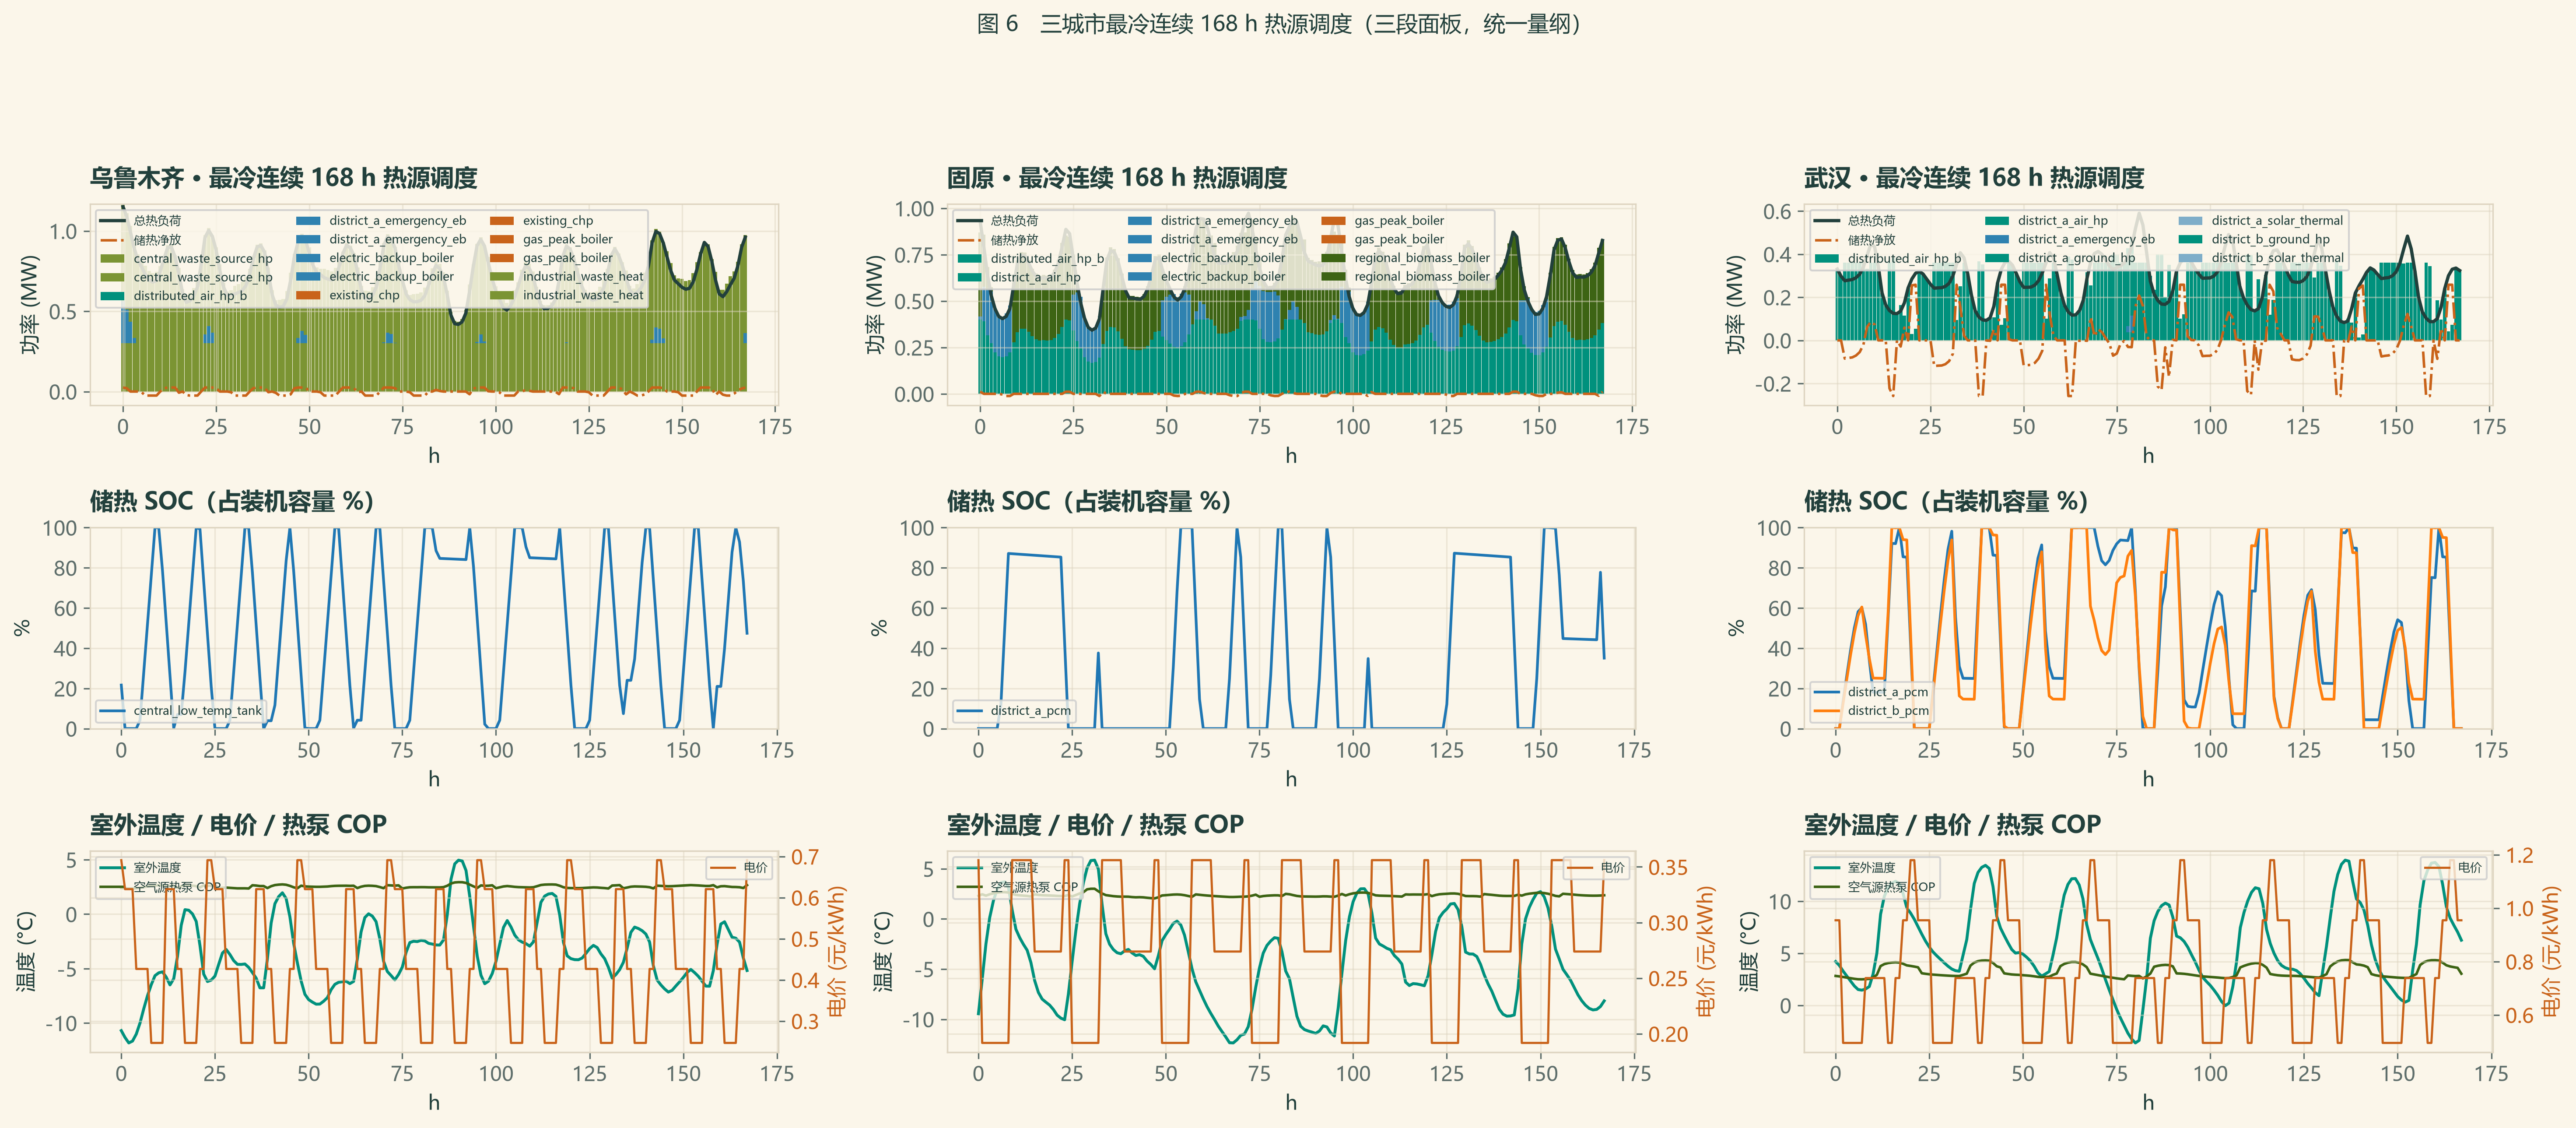
\includegraphics[width=0.98\textwidth,height=0.54\textheight,keepaspectratio,trim=0 0 0 100,clip]{media/code-results/fig06_coldest_168h_dispatch.png}
\caption{最冷连续168 h调度}
\label{fig:code-cold168}
\end{figure}

\begin{figure}[H]
\centering
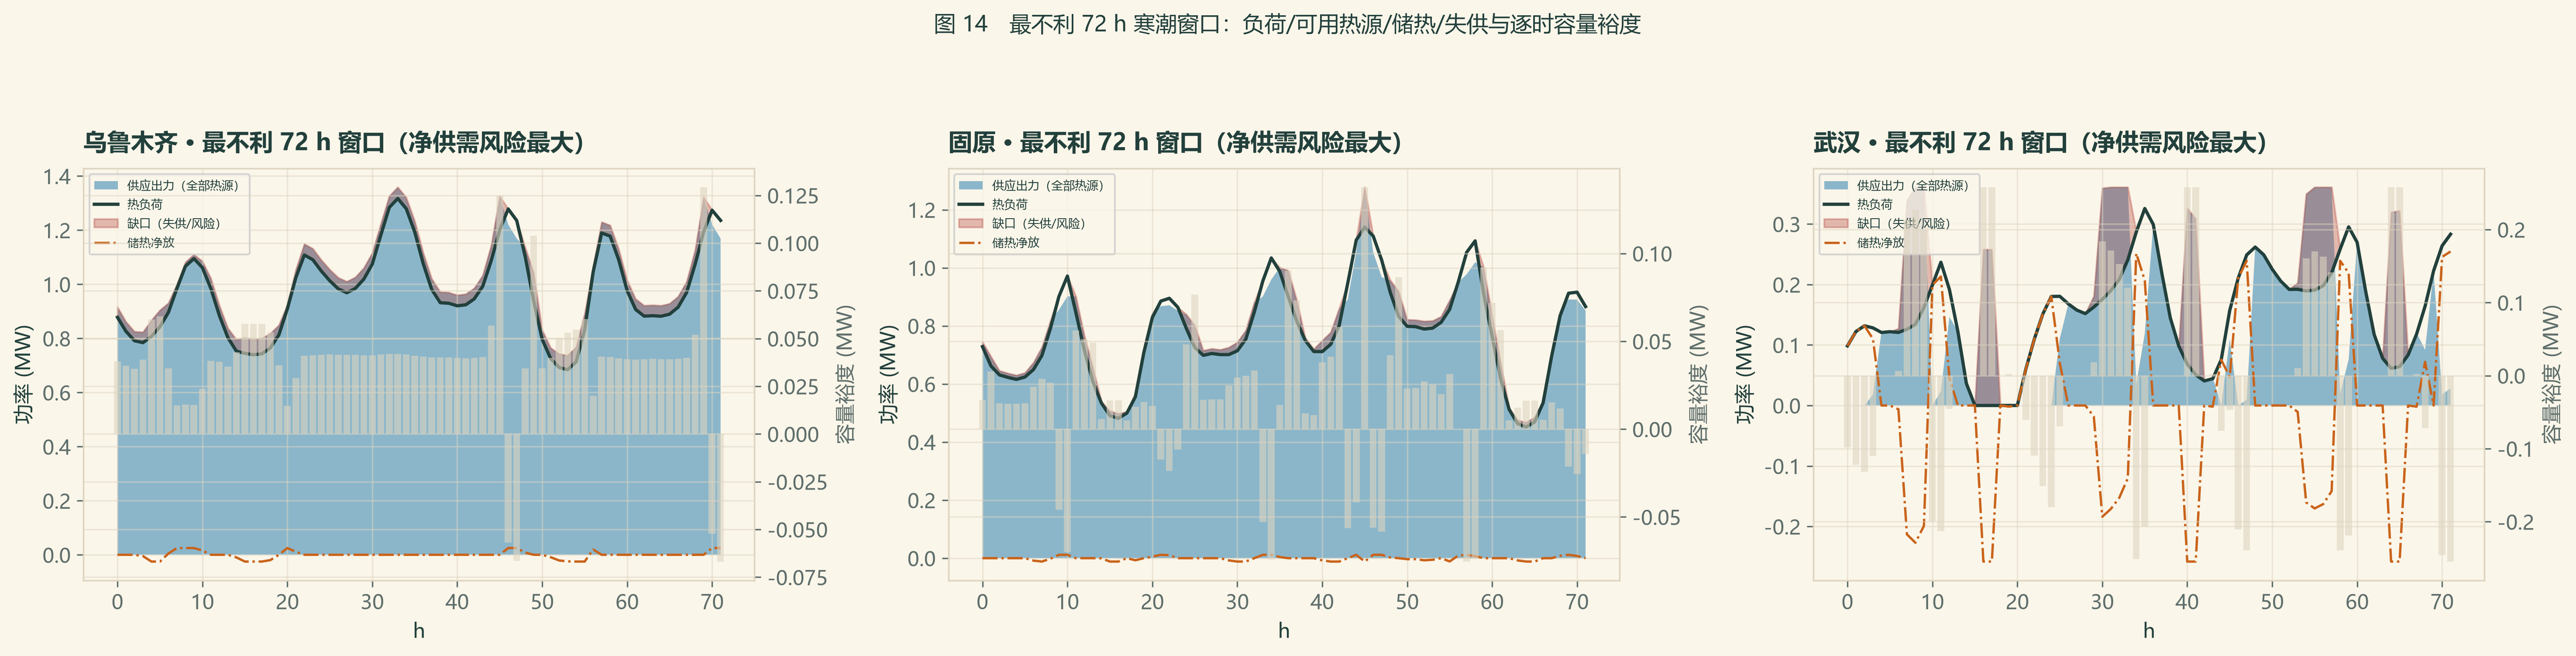
\includegraphics[width=0.98\textwidth,height=0.43\textheight,keepaspectratio,trim=0 0 0 100,clip]{media/code-results/fig14_worst_72h_resilience.png}
\caption{最不利72 h韧性窗口}
\label{fig:code-worst72}
\end{figure}

与“单年或五年聚合代表时段、最小化平均成本”的基准相比，多气象年回放使用约3---4倍代表行数，5个气象年的容量审计均通过，最差场景失供率仍为0。消融实验、压力测试和数据可靠性分级见图\ref{fig:alg-ablation}。

\begin{figure}[H]
\centering
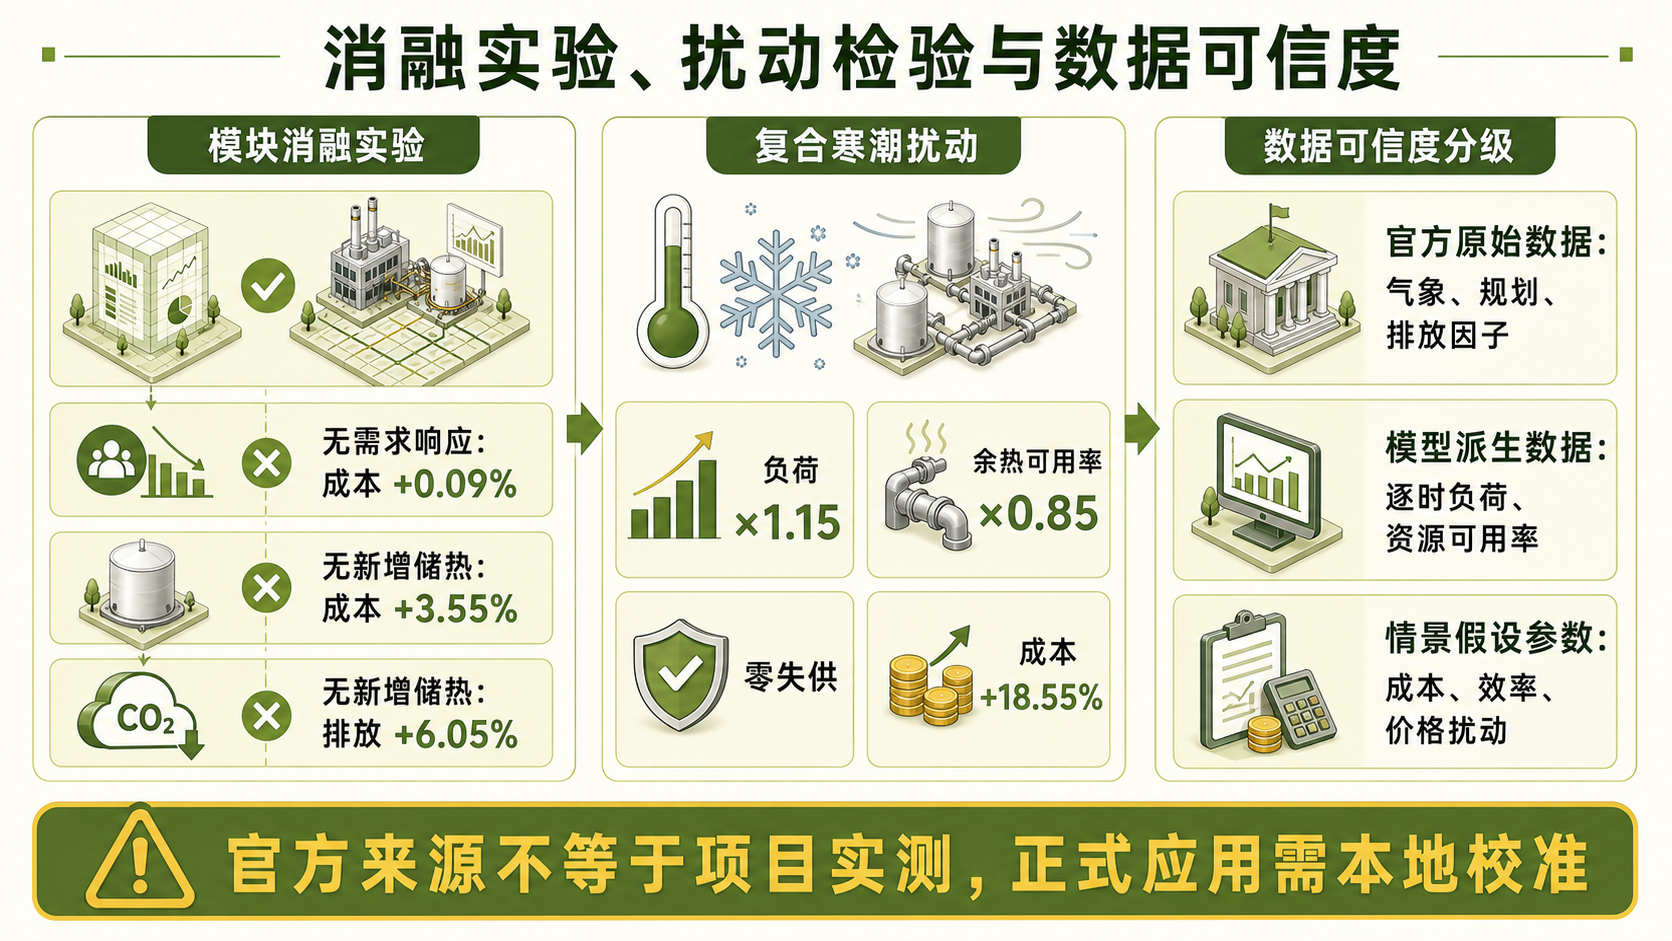
\includegraphics[width=0.76\textwidth,height=0.30\textheight,keepaspectratio]{media/algorithm-revision/fig5.png}
\caption{消融实验、扰动检验与数据可靠性}
\label{fig:alg-ablation}
\end{figure}

\subsection{数据基础与适用范围}

气象数据采用NASA POWER格点逐时数据，空间分辨率为$0.5^{\circ}\times0.625^{\circ}$，不作为地面站实测数据。热工参数、项目容量和政策边界取自标准、批复与政府文件；设备成本、燃料价格等作为情景假设并给出区间。数据记录包括来源、链接、检索时间、单位、分辨率、换算公式和适用局限。

碳排放按逐时电力排放因子计算，由输入时序列\texttt{grid\_emission\_factor}逐时读取，不作常数处理。本次补充验证三场景回放所用该列的取值个数为 17---19 个，范围为 $0.43$---$0.69$~kg~CO$_2$/kWh，全年均值约 $0.535$---$0.546$。作为参考，2023 年全国电力平均排放因子为 0.5306~kg~CO$_2$/kWh，新疆、宁夏和湖北的省级年度参考因子分别为 0.6021、0.6187 和 0.4044~kg~CO$_2$/kWh。同包交付的《仿真结果数据表》中，共享容量原型对照单独采用湖北省年度因子 0.4044，与主场景的逐时因子分属不同登记值；改用统一常数因子重算属于后续可补充的对照工作。三场景均为代表性多节点系统，缩比系数仅用于规模换算，不表示对城市地理系统的完整复刻，横向比较采用单位指标。

\subsection{小结}

算法采用$\varepsilon$-约束处理成本与碳排放的多目标关系，以硬边界约束可靠性，并以$\lambda$-CVaR描述风险态度。三个场景采用同一条“代表时段投资---运行联合规划，再冻结投资完成全季运行校核”的管线，规划层与回放层分别报告求解状态与间隙。多尺度耦合通过节点---温位聚合、用户侧等效热状态以及城市、区域与用户层之间的共享变量实现。

本次补充验证的对应记录见表\ref{tab:alg-supplement}与同包交付的《仿真结果数据表》，其中三个场景的冻结投资全年回放均取得已证最优或容差内最优解，失供率为 0。前述历史报告值的逐行核验状态见相应表格的「来源状态」列。

当前主要成果为成本---碳排放二维$\varepsilon$-约束扫描得到的候选方案集：按有限档位逐档重解，每档报告可行值与对偶界，其中乌鲁木齐中间档的部分点属时限内近似解。该集合是有限档位上的候选解，不等同于对连续前沿的完整刻画。后续可进一步开展三维Pareto扩展、省级排放因子重算，以及连续温位、C\&CG、Benders分解和在线MPC等方法的计算研究。


\clearpage
\section{数据体系与模型验证}

数据、标定与验证部分不承担优化求解任务，而用于保证输入参数可追溯、模型结果可复现以及工程结论可验证。本文按照“数据准入---参数标定---样本外验证---工程验收---结果输出”的流程组织验证体系。

如图\ref{fig:model-095}所示，数据准备、参数标定、样本外验证和工程验收形成逐层递进的可信度证据链。

\begin{figure}[H]
\centering
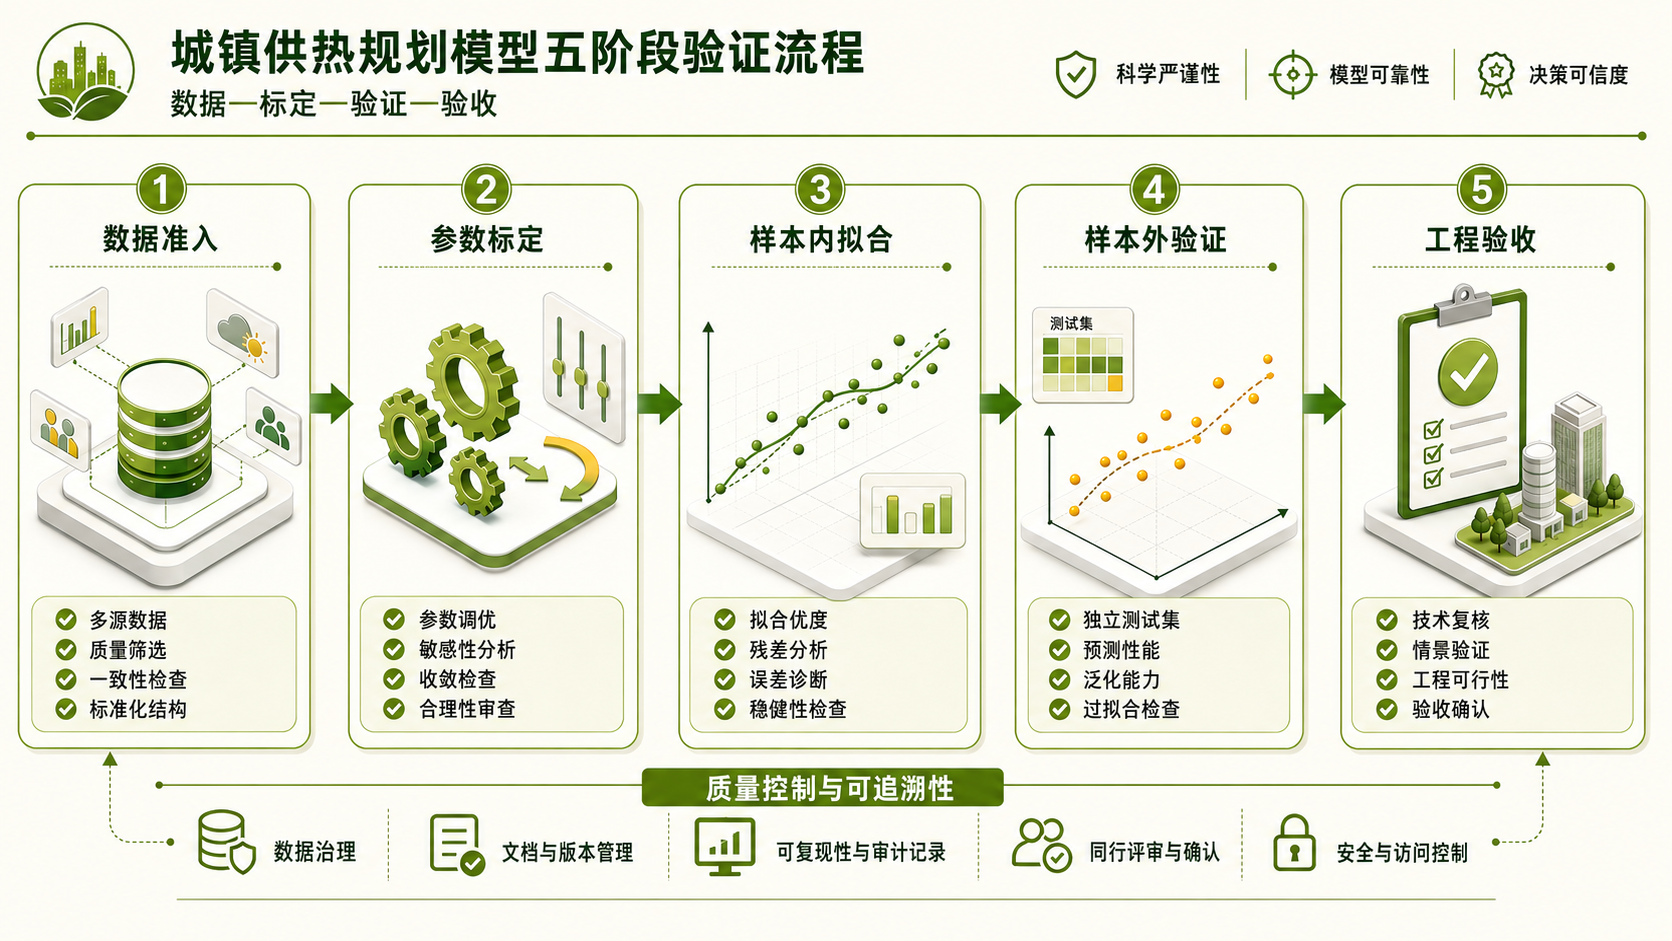
\includegraphics[width=0.714\textwidth,height=0.34\textheight,keepaspectratio]{media/model-figures/095.jpg}
\caption{数据—标定—验证—验收}
\label{fig:model-095}
\end{figure}

\subsection{场景配置清单}

\begin{longtable}[]{@{}p{0.07\textwidth}p{0.26\textwidth}p{0.14\textwidth}p{0.16\textwidth}p{0.17\textwidth}@{}}
\caption{模块启用与验证情况}\label{tab:20}\\
\toprule\noalign{}
\begin{minipage}[b]{\linewidth}\raggedright
场景
\end{minipage} & \begin{minipage}[b]{\linewidth}\raggedright
模块
\end{minipage} & \begin{minipage}[b]{\linewidth}\raggedright
代码支持
\end{minipage} & \begin{minipage}[b]{\linewidth}\raggedright
本次启用
\end{minipage} & \begin{minipage}[b]{\linewidth}\raggedright
结果验证
\end{minipage} \\
\midrule\noalign{}
\endfirsthead
\endhead
\bottomrule\noalign{}
\endlastfoot
C1 & 退役、余热、热泵、管网、储热 & 支持 & 启用 & 联合求解及全季校核 \\
C1 & BTES多年动态、连续水力 & 支持 & 未启用 & 未形成算例结果 \\
C2 & 选址、分配、燃料库存、微网 & 支持 & 启用 & 锚定投资后全季校核 \\
C2 & 污染物、可负担性、运维可达性 & 支持 & 部分启用 & 仅报告已启用指标 \\
C3 & 供热形态、热泵、储热、配电 & 支持 & 启用 & 锚定投资后全季校核 \\
C3 & 热湿、结露、噪声、地源平衡 & 支持 & 未启用 & 作为扩展模块说明 \\
\end{longtable}


\subsection{最小数据集}

\begin{longtable}[]{@{}
  >{\raggedright\arraybackslash}p{(\columnwidth - 6\tabcolsep) * \real{0.1442}}
  >{\raggedright\arraybackslash}p{(\columnwidth - 6\tabcolsep) * \real{0.1549}}
  >{\raggedright\arraybackslash}p{(\columnwidth - 6\tabcolsep) * \real{0.3237}}
  >{\raggedright\arraybackslash}p{(\columnwidth - 6\tabcolsep) * \real{0.3771}}@{}}
\caption{最小数据集}\label{tab:21}\\
\toprule\noalign{}
\begin{minipage}[b]{\linewidth}\raggedright
数据类别
\end{minipage} & \begin{minipage}[b]{\linewidth}\raggedright
建议分辨率
\end{minipage} & \begin{minipage}[b]{\linewidth}\raggedright
共用字段
\end{minipage} & \begin{minipage}[b]{\linewidth}\raggedright
场景专用字段
\end{minipage} \\
\midrule\noalign{}
\endfirsthead
\endhead
\bottomrule\noalign{}
\endlastfoot
GIS/资产 & 设备、管段、建筑级 & 坐标、道路、长度、管径、年代、地块 & C1
既有状态；C2 村镇/道路；C3 地下空间/声敏点 \\
运行监测 & 5--60 min & 热量、流量、压力、供回水温度、电功率 & C1 CHP
工况；C3 室内温湿度与启停 \\
热源资源 & 15 min--日 & 可用量、源温、检修、位置 & C1 余热停产；C2
生物质来源；C3 水源/地源许可 \\
建筑负荷 & 15 min--小时 & 面积、用途、末端、热量、室温 & C2
收入/运维；C3 占用、冷量、热水、湿度 \\
气象 & 小时 & 干球温度、风、辐照 & C3 湿球/相对湿度、结霜工况 \\
电力/碳 & 小时 & 电价、边际碳因子、变压器容量 & C2/C3
台区增容与停电影响 \\
成本/寿命 & 年度 & CAPEX、OPEX、寿命、残值、碳价 &
退役、物流、仓储、班组、声学治理 \\
\end{longtable}


\subsection{参数标定与外部验证}

参数来源按``实测监测---设备/设计资料---同行评审工程文献---合理区间假设''四级记录。能够获得的气象、负荷、资产、价格和碳因子使用目标城市数据；建筑
等效热容、管段热损、水力阻力、CHP 运行域、储热和 BTES
参数若无法实测，则采用公开工程参数作为中心值，并设置上下限开展敏感性分析。SSRN
预印本\supcite{3}用于补充相关技术信息；温位匹配、低温网和 BTES
的关键参数依据目标项目数据、工程资料或同行评审文献确定，不采用文献单点值作为全国统一参数。

有足够数据时，使用未参与参数辨识的年份或天气序列做样本外验证；数据不足时，至少保留一个寒潮连续时段和一个过渡期时段，并公开参数区间。三个场景均采用统一的守恒、求解和验收规则完成连续供暖季计算；受可用数据范围影响，各场景参数标定精度分别说明，不把代理数据表述为现场实测数据。

如图\ref{fig:model-096}所示，本图仅说明验证方法；样本内参数辨识与样本外气象回放分开实施，实际精度以求解日志和逐时记录为准。

\begin{figure}[H]
\centering
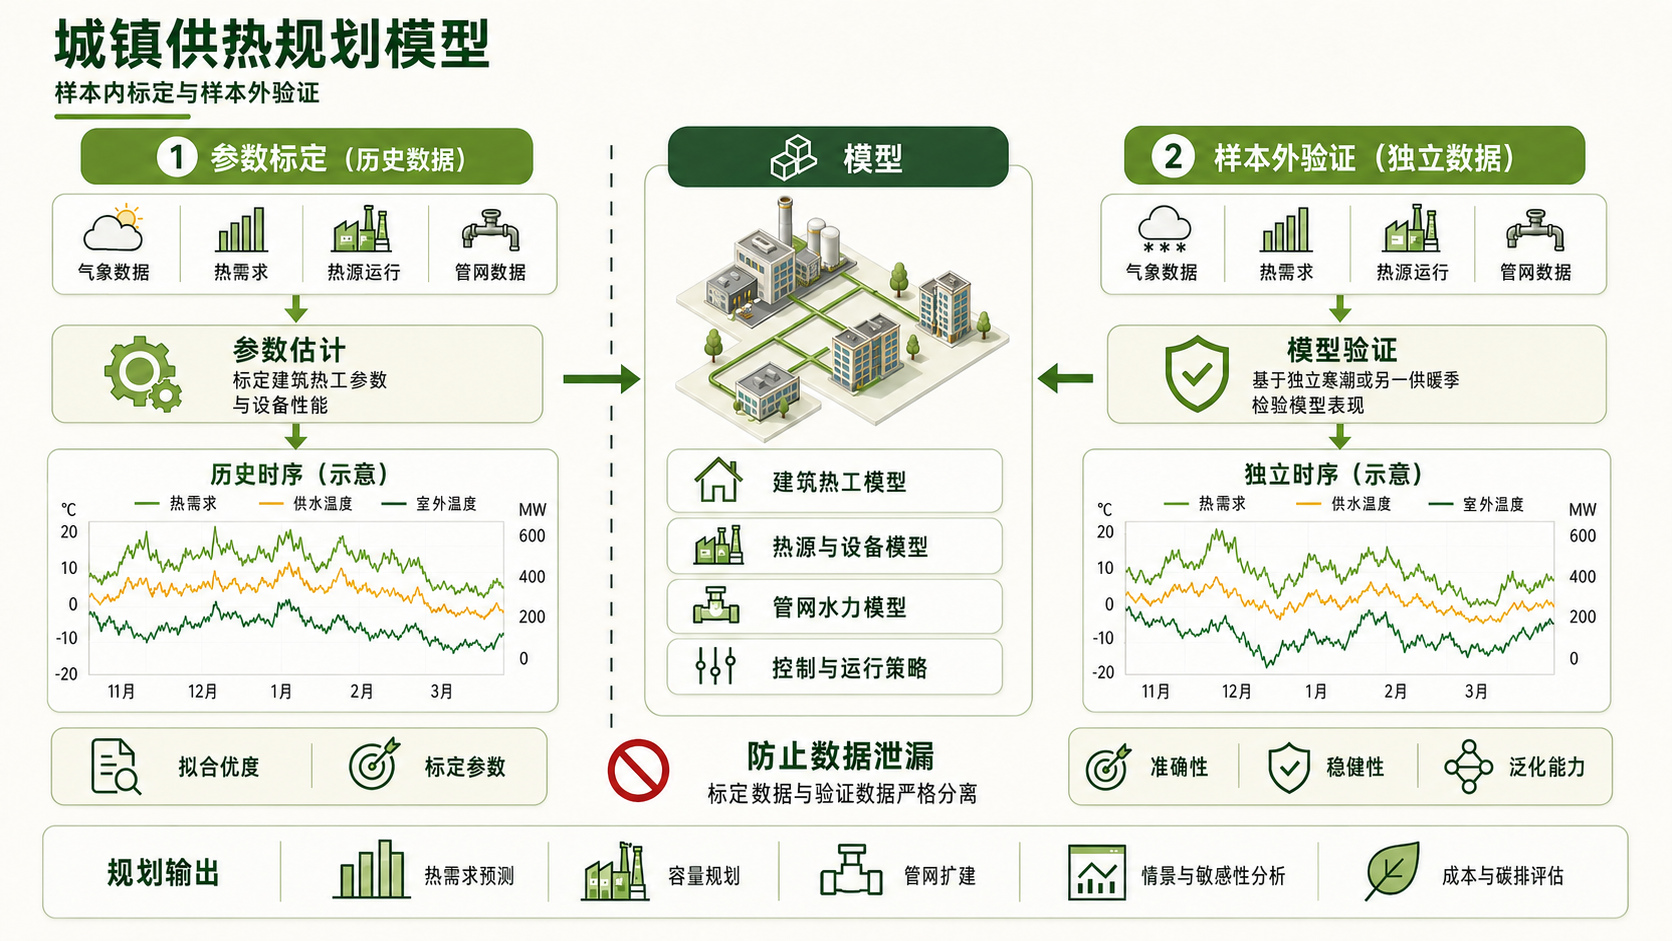
\includegraphics[width=0.714\textwidth,height=0.34\textheight,keepaspectratio]{media/model-figures/096.jpg}
\caption{样本内与样本外验证方法示意}
\label{fig:model-096}
\end{figure}

\subsection{工程验收标准}

\begin{enumerate}
\def\labelenumi{\arabic{enumi}.}
\tightlist
\item
  所有节点、载体、库存和状态方程在容差内闭合，单位和时间权重一致。
\item
  正常情景无计划外失供；已纳入测试的极端和 N−1
  情景满足应急室温、持续时间与恢复要求。
\item
  管网温度、压力、流速和泵工况通过非线性复核；对启用了启停与爬坡模块的设备，再校核最小开停时间、爬坡和部分负荷边界。
\item
  C1 的降温与末端改造同步，最大热源 N−1 通过；BTES 和关键管段 N−1
  启用时满足相应要求。
\item
  启用 C2
  对应模块时，生物质质量---热量---库存闭合，污染物达标，物流中断和微网孤岛通过，供热费用可负担。
\item
  启用 C3
  对应模块时，占用温湿度、升温时间、湿冷除霜、声环境、地源平衡与配电峰值达标。
\item
  成本、碳、资源、折现率和不确定性情景参数（或启用预算集时的\(\Gamma\)）的敏感性结论稳定，推荐方案不是单点参数偶然结果。
\item
  所有差分状态式均以 \(\Delta x/\Delta t\)
  表示变化率；孤岛、热回收、热损和储能账本不存在虚拟供给或重复计量。
\item
  政策淘汰期限、清洁供热占比、污染物总量、年度投资和供热季禁施工窗口均通过项目配置文件加载并满足。
\end{enumerate}


建筑入口热量、聚合节点等效热状态及生活热水（启用时）在时间权重下闭合。可回查的全年回放记录中，三个场景的数值审计最大约束违反量依次为$9.963\times10^{-7}$、$9.997\times10^{-7}$和$8.837\times10^{-7}$，变量界最大违反量依次为$2.629\times10^{-13}$、$1.2596\times10^{-8}$和$8.273\times10^{-7}$，均在登记的绝对容差$10^{-6}$、相对容差$10^{-8}$与缩放违反上限$1.0$之内；三场景的储热状态方程最大残差依次为$1.208\times10^{-13}$、$5.684\times10^{-13}$和$3.961\times10^{-13}$~kWh，各储热装置的初末状态与逐时极值登记于同包交付的《仿真结果数据表》。


目标温位下的节点供热、回水温度和最小供回水温差按已启用模块检查；连续水力和房间级温度属于工程扩展校核。

如图\ref{fig:model-097}所示，热量、电力、库存和状态方程的残差均需控制在统一数值容差以内。

\begin{figure}[H]
\centering
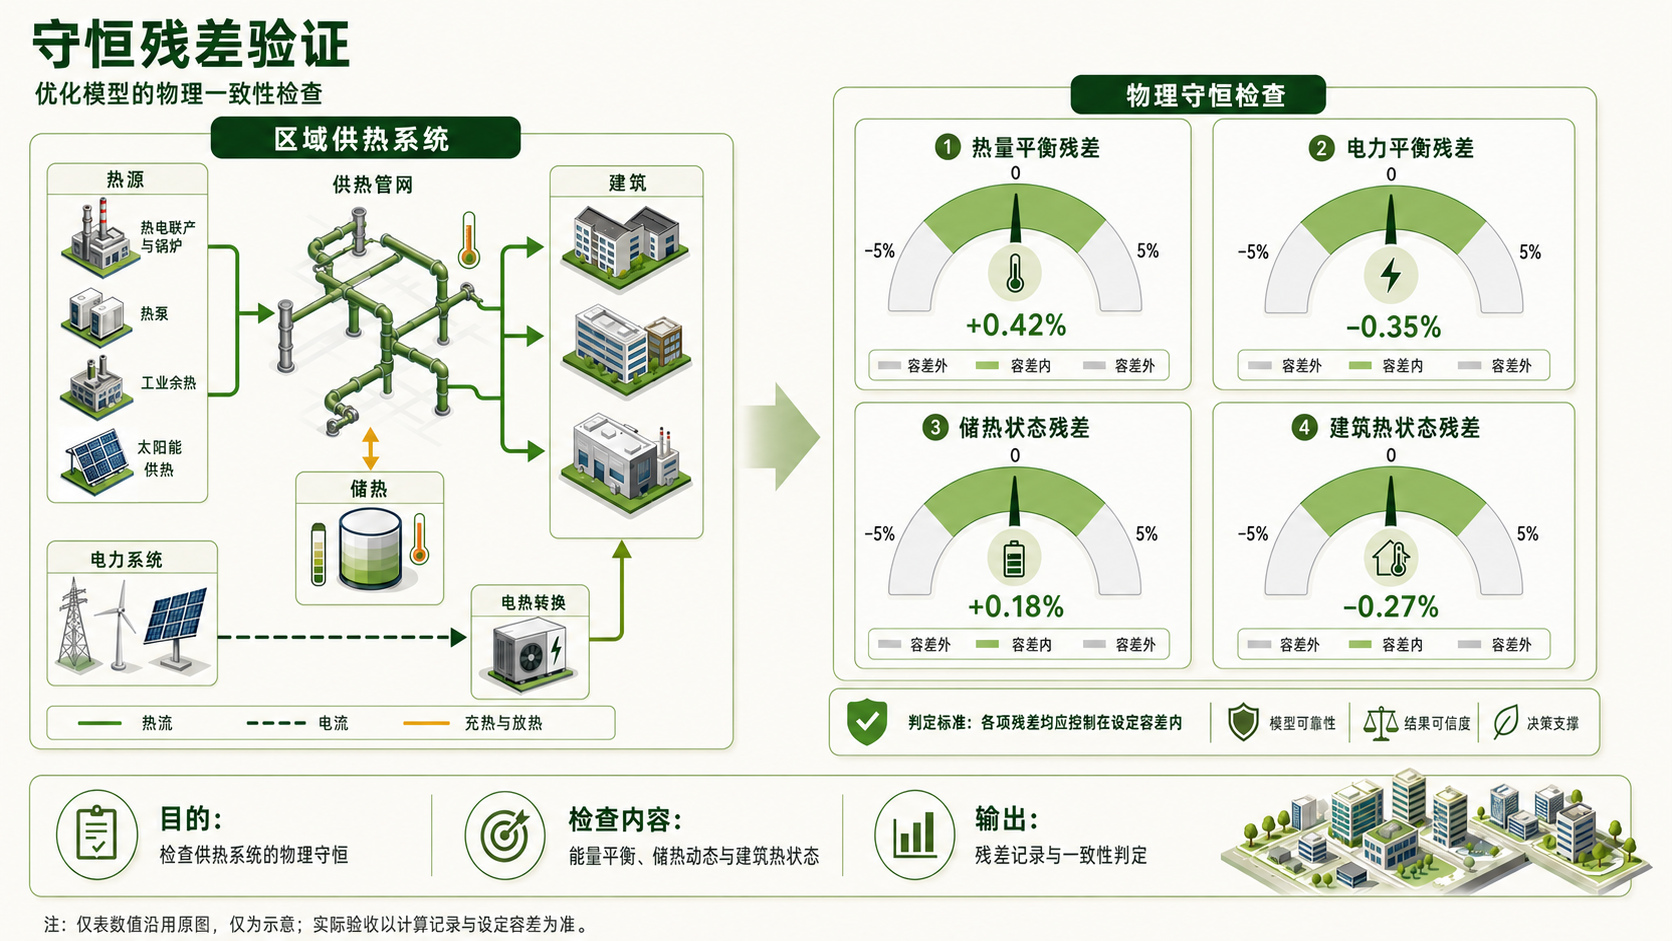
\includegraphics[width=0.714\textwidth,height=0.34\textheight,keepaspectratio]{media/model-figures/097.jpg}
\caption{守恒残差容差示意（图内仪表数值为示意，实际验收以计算记录与设定容差为准）}
\label{fig:model-097}
\end{figure}

图\ref{fig:model-097}为容差判定方式的示意，其表盘读数不是本次算例的实测残差；可回查的逐时残差与状态审计登记于表\ref{tab:alg-supplement}与原附录记录，工程复核仍以计算记录为准。

需求响应不超过计量控制覆盖和参与率，并在退出或同步恢复情景下仍可运行。


三个场景均完成完整供暖季数值结果，并分别报告规划求解、连续时序回放与压力测试的求解状态；机器验收以逐项验收记录为准。仅在连续水力、声学、地源等专业复核模块上说明实际启用范围。

如图\ref{fig:model-098}所示，最大流量管段、最远换热站和最不利建筑是工程复核的重点断面；该图为复核流程示意，四类断面的状态标识表示校核环节，实际结论以工程复核记录为准。

\begin{figure}[H]
\centering
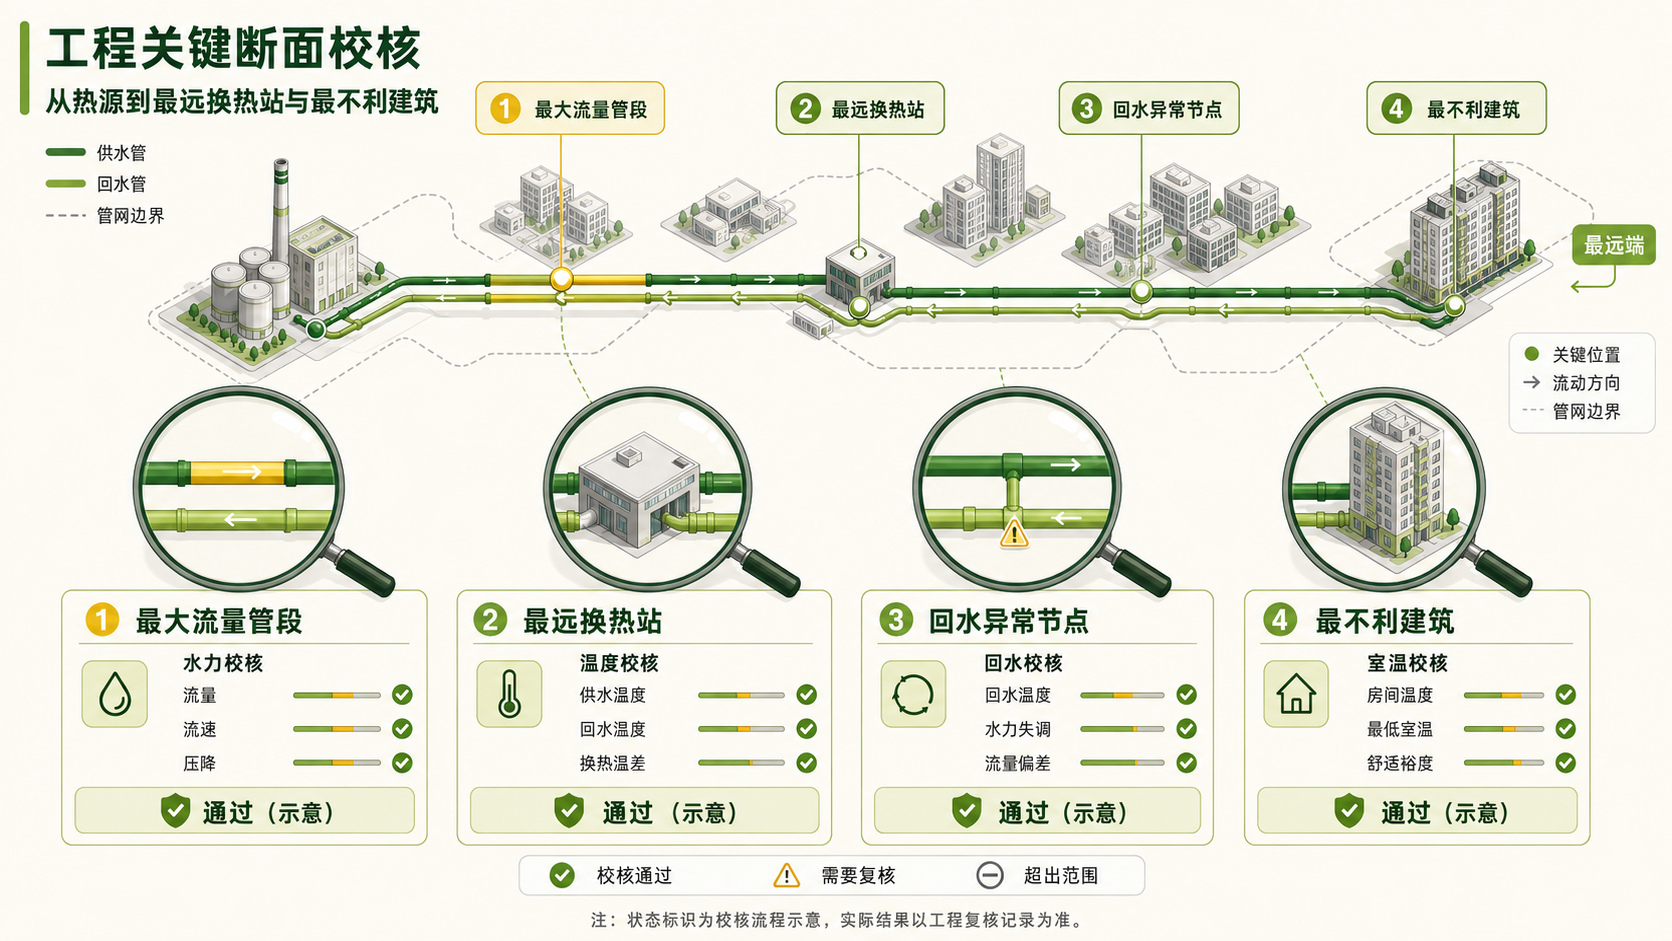
\includegraphics[width=0.714\textwidth,height=0.34\textheight,keepaspectratio]{media/model-figures/098.jpg}
\caption{工程关键断面校核流程示意（状态标识为示意，实际结果以工程复核记录为准）}
\label{fig:model-098}
\end{figure}

\subsection{对照与消融分析}

本次对照分析采用V4全年算例及其原有时间权重。每移除一个模块，均重新求解投资与运行变量，而非只在既定方案上删除相应成本项。已完成的对照包括去除需求响应、去除新增储热和去除火用失配惩罚；另对三个场景开展电价、负荷、碳价和资源可用率敏感性分析，并在冻结投资后完成复合寒潮测试。未实际求解的对照不作为结果报告。

完整模型年化目标为95.620万元。去除新增储热后，年化成本增加3.55\%，碳排放增加6.05\%；复合寒潮下运行目标值增加18.55\%，同时保持零失供。该指标含年化投资与惩罚项，与能源现金支出分别核算；该组V4结果与三城市供暖季推荐方案分开解释；两者统计范围不同，不直接比较。上述消融与压力测试数值为既有实验记录，其求解日志未随附，本表按历史报告值列出。

如图\ref{fig:model-099}所示，模型保留影响规划结论的关键机理，并将高精度局部问题放到求解后校核。

\begin{figure}[H]
\centering
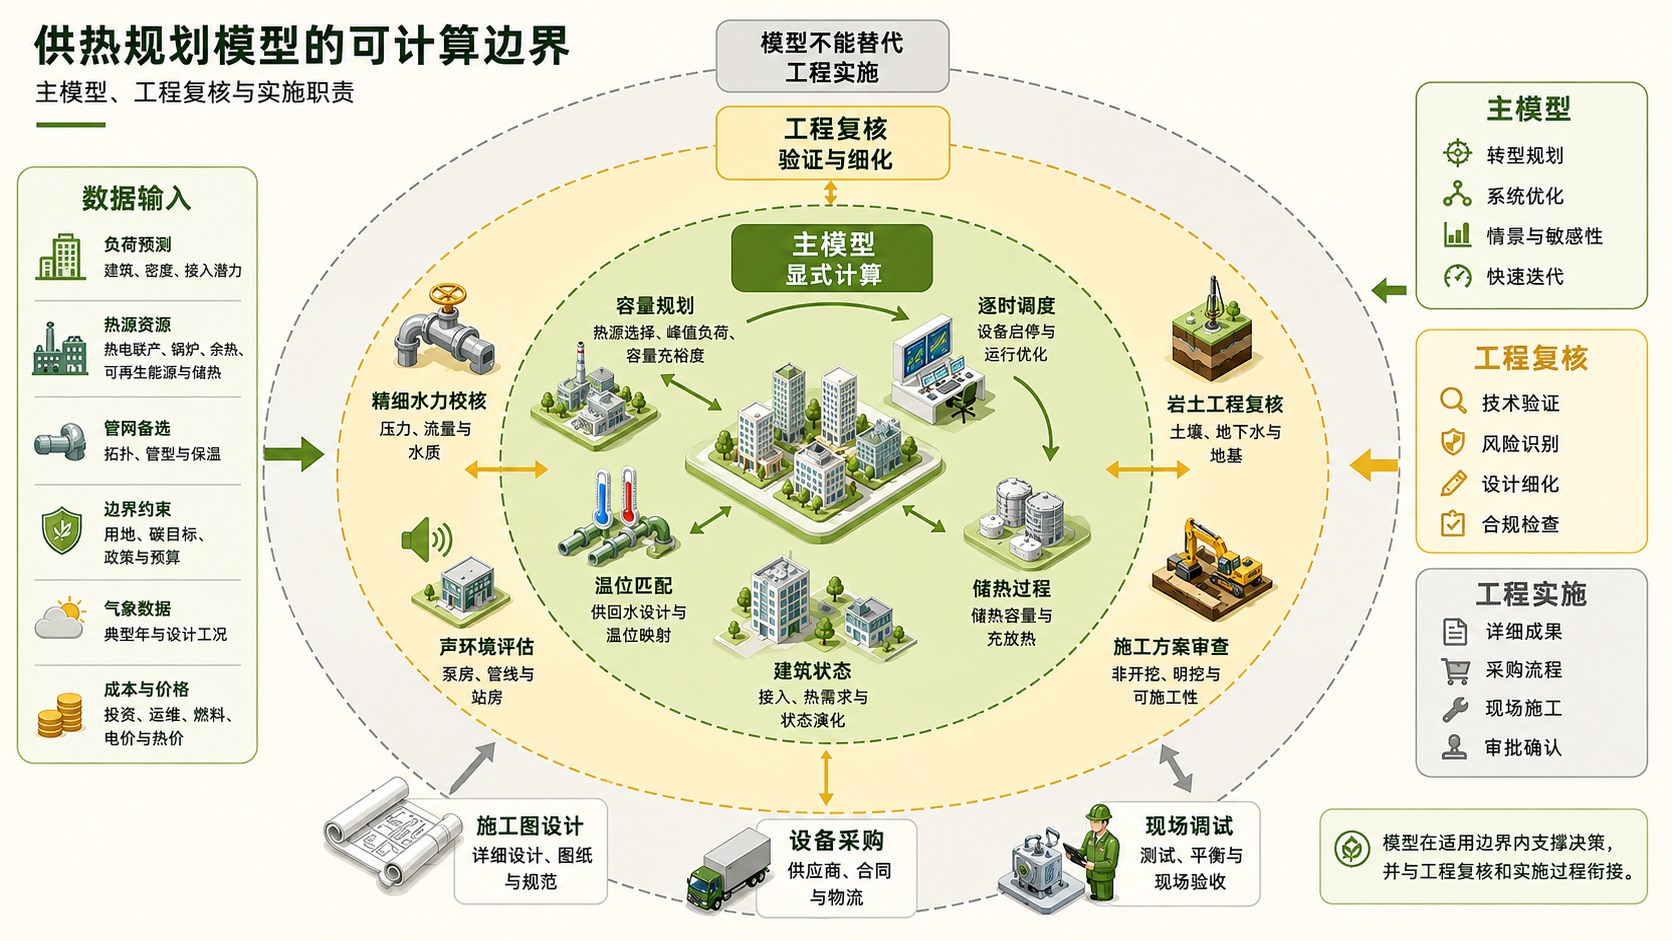
\includegraphics[width=0.714\textwidth,height=0.34\textheight,keepaspectratio]{media/model-figures/099.jpg}
\caption{可计算边界}
\label{fig:model-099}
\end{figure}

\subsection{标准化成果}

统一输出包括：数据字典与参数来源、候选链/拓扑清单、三个场景的容量配置、完整供暖季逐时调度、场景专用指标、压力测试、敏感性和校核记录。交付包根目录提供\texttt{README.md}，说明目录结构、Python依赖、Windows运行命令、三场景配置位置和供暖季输入位置；批量入口使用当前解释器调用，避免写死Python安装路径。已有结果可通过求解日志、逐时输出和验收记录交叉检查。


\subsection{结果可视化与后处理}

图表统一配色、字体和单位，主要展示系统能流与资产拓扑、节点边际热价、源荷匹配与储热状态、代表周设备出力、成本---碳排候选集，以及关键情景下的室温、回水、压力和失供量。边际热价仅根据固定整数方案重求解后能量平衡约束的对偶值解释，不采用MILP根节点对偶值。图表同时标明数据版本、场景、时间分辨率、单位和数据性质，并保留同源数据以供复核。


\clearpage
\section{模型应用与决策分析}

本文模型面向供热转型规划、项目比选、投资安排、风险评估和政策分析，输出容量配置、建设时序、运行指标及工程约束校核结果。

\subsection{区域供热转型规划}

模型可比较热源结构、管网温位、储热和建筑改造路径，并依据生命周期成本、碳排放、峰值化石依赖率与可靠性指标，确定各阶段资产的建设、保留、改造和退役安排。

\subsection{项目方案比选}

候选方案可在相同负荷、气象、价格和可靠性边界下比较，评价设备投资、运行费用、温位适配、配电容量、建筑舒适和故障保供，并识别容量余量与关键瓶颈。

\subsection{改造时序与投资安排}

在年度预算、施工能力和投产时间约束下，模型形成分年度建设清单，并分析项目延期对峰值容量、运行成本和备用需求的影响。

\subsection{极端情景与风险评估}

固定投资方案后，对寒潮、资源中断、价格变化、需求响应退出及关键故障进行重调度，检查失供、室温、配电峰值和储热状态，确定备用容量和应急运行边界。

\subsection{政策与低碳路径评估}

通过调整碳约束、清洁热比例、补贴、能源价格和可靠性门槛，可生成成本---减排Pareto候选集。政策判断仍需结合地方财政、资源条件和居民可负担性。

\subsection{应用流程与成果输出}

应用流程包括数据整理、候选方案求解、压力测试和工程校核。成果用于规划决策，不能替代施工图、水力平衡、设备选型、地质勘察和现场调试。

\clearpage
\section{模型创新、局限与结论}

\subsection{模型创新}

核心创新一：联合优化热源温位匹配、管网拓扑和输送容量，并以温位匹配率与末端适配率进行校核。

如图\ref{fig:model-125}所示，温位选择与管网拓扑同步优化，使热源品质、输送路径和终端需求在同一模型中匹配。

\begin{figure}[H]
\centering
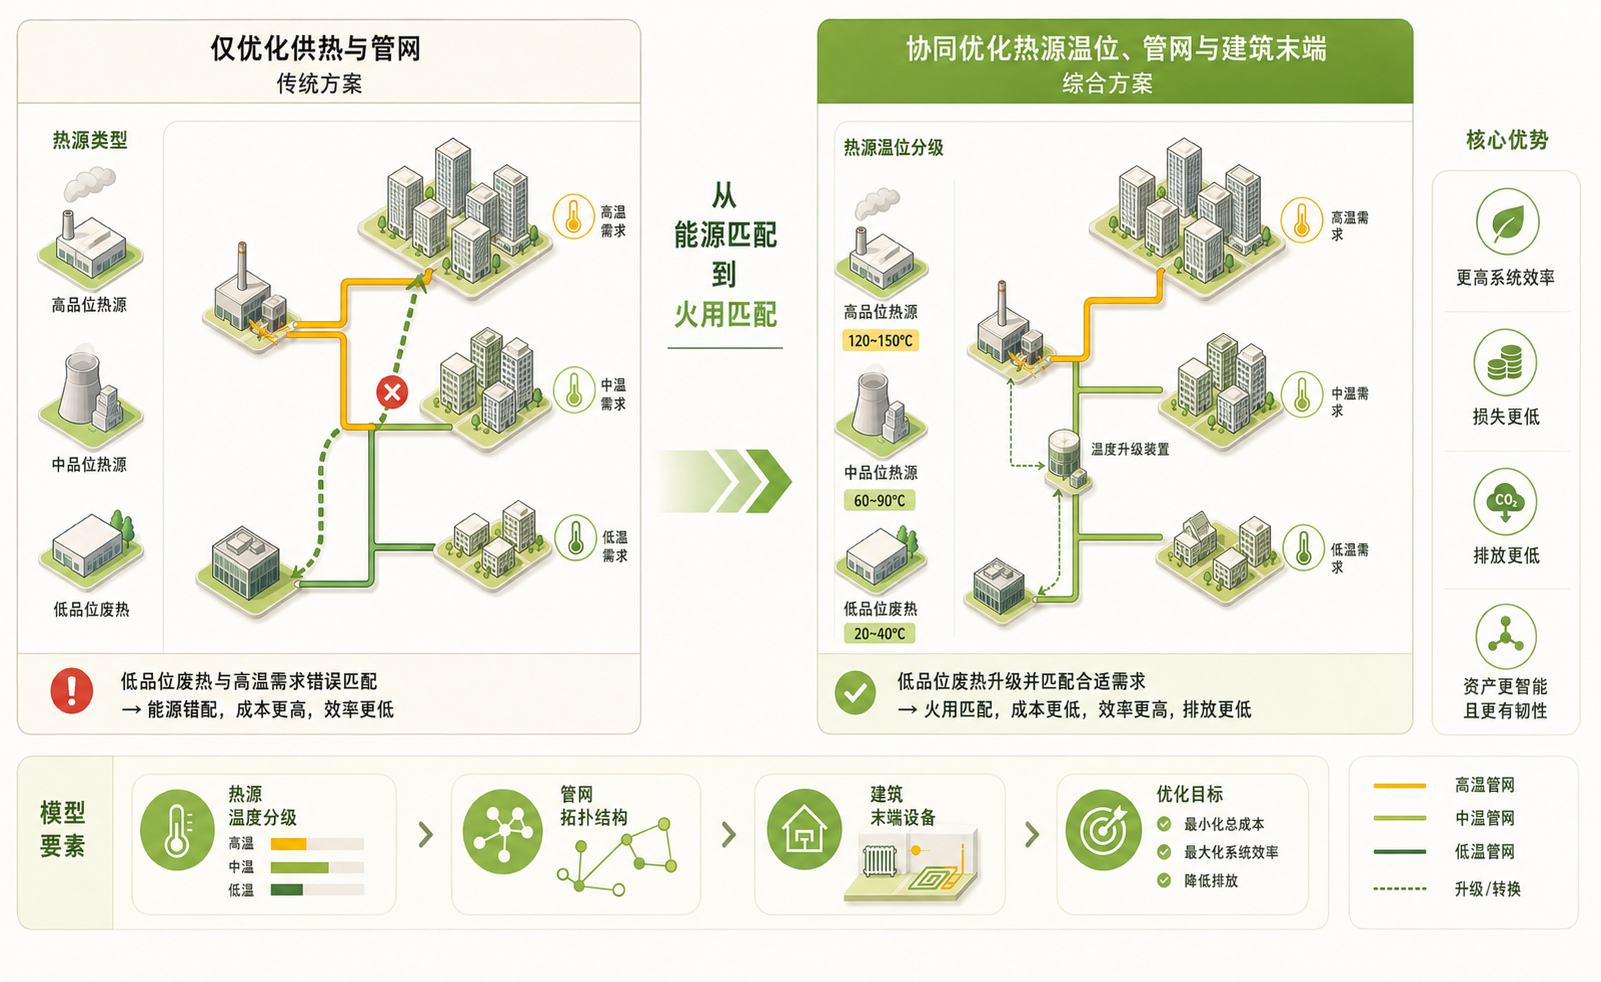
\includegraphics[width=0.714\textwidth,height=0.34\textheight,keepaspectratio]{media/model-figures/125.jpg}
\caption{创新点一：温位 + 拓扑联合优化}
\label{fig:model-125}
\end{figure}

核心创新二：设置骨干管网“保留运行---改造运行---退出主运行”三态，统一比较存量资产利用、温位迁移、热损和泵耗。

如图\ref{fig:model-126}所示，管网保留、改造和退役三种状态被内生选择，从而形成可分阶段实施的网络方案。

\begin{figure}[H]
\centering
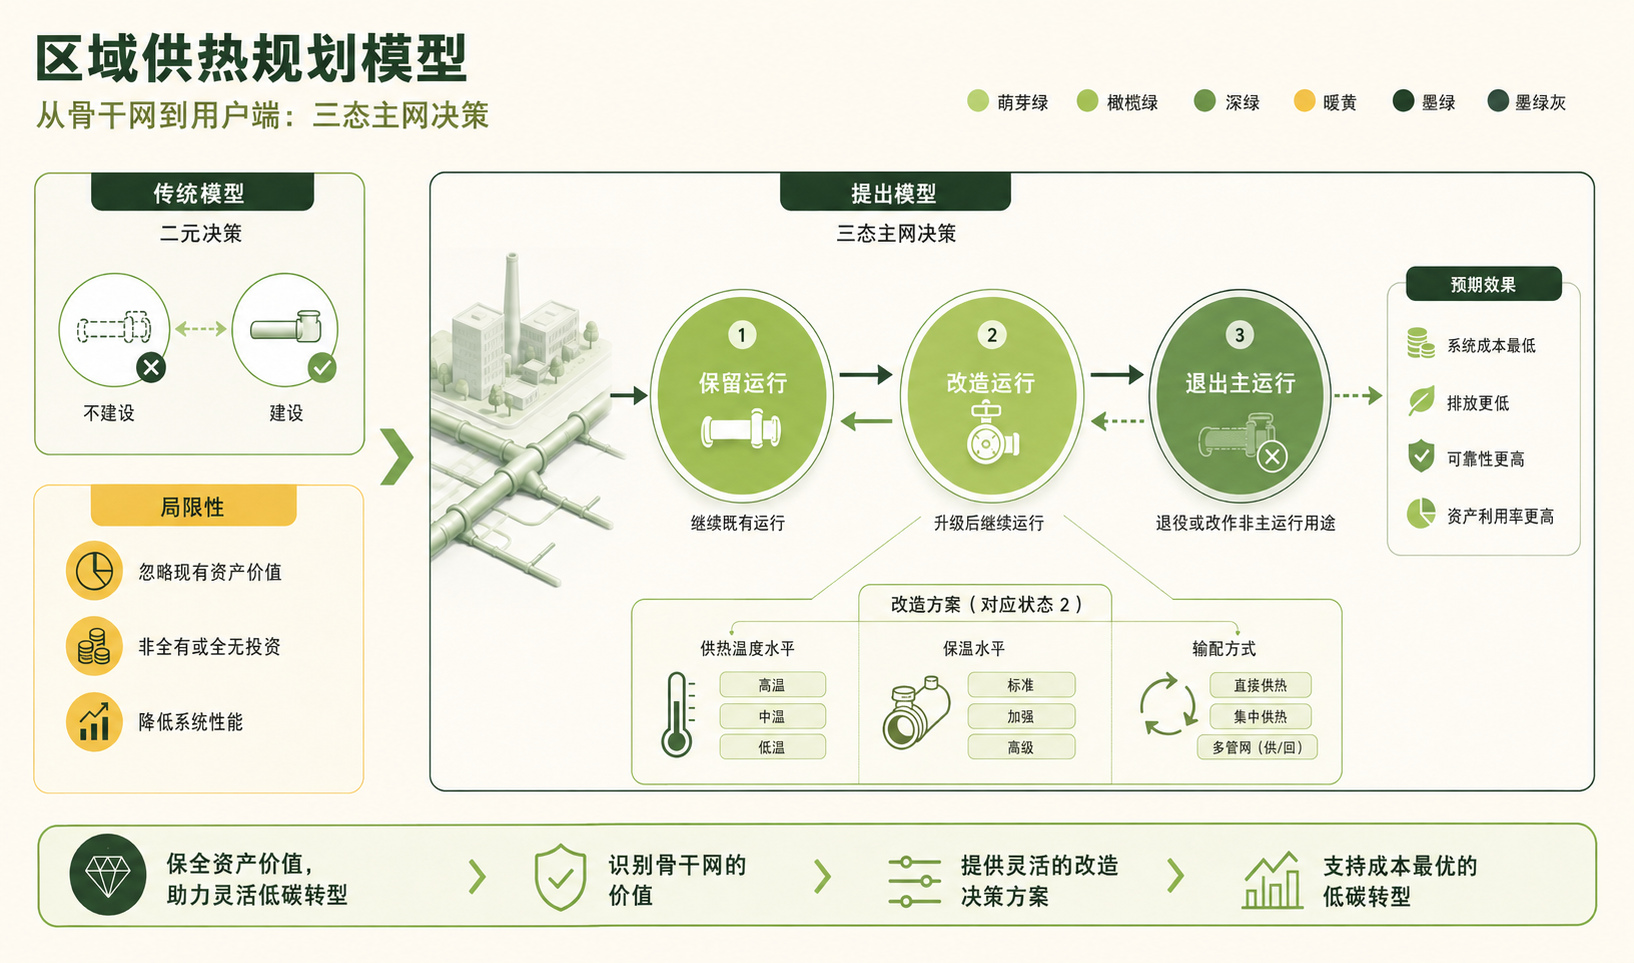
\includegraphics[width=0.714\textwidth,height=0.34\textheight,keepaspectratio]{media/model-figures/126.jpg}
\caption{创新点二：管网三态}
\label{fig:model-126}
\end{figure}

核心创新三：将化石热源改造与退役作为决策变量，以可靠容量、建筑负荷、节点供热和应急保供条件确定分年度退出路径。

如图\ref{fig:model-127}所示，化石热源退役时点由系统约束和经济权衡决定，避免人为预设替代节奏。

\begin{figure}[H]
\centering
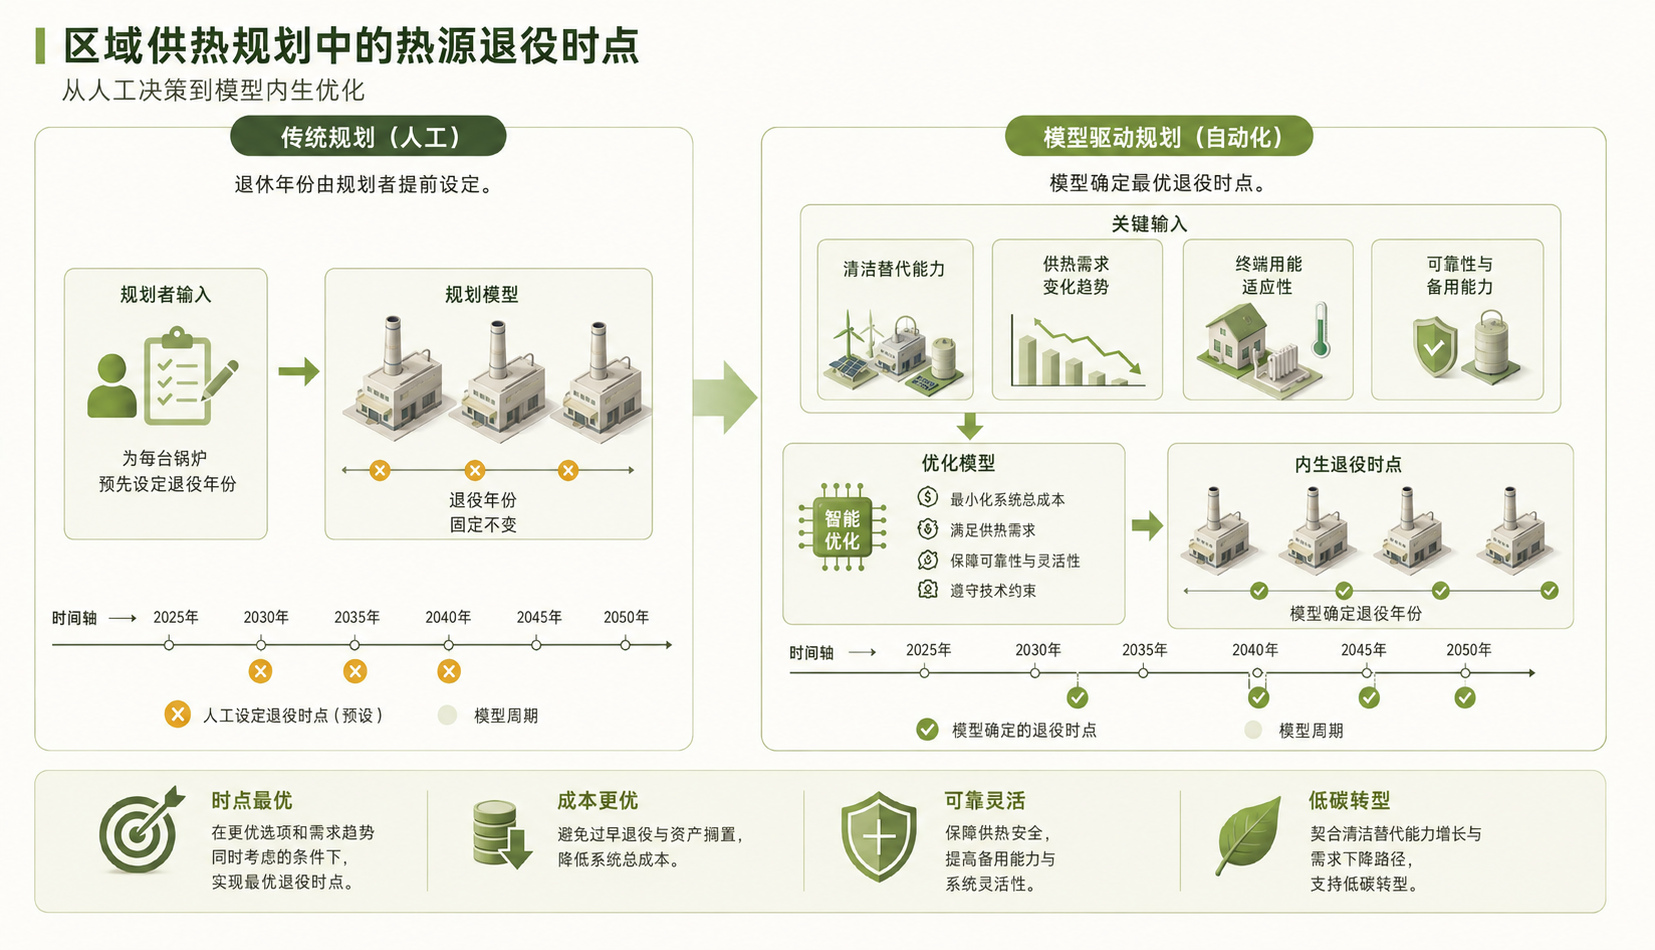
\includegraphics[width=0.714\textwidth,height=0.34\textheight,keepaspectratio]{media/model-figures/127.jpg}
\caption{创新点三：化石热源内生退役}
\label{fig:model-127}
\end{figure}
核心创新四：将源、网、荷、储运行与用户侧等效热状态置于同一逐时账本中，需求响应按允许窗口转移负荷与恢复负荷，并由热源与储热共同响应。

如图\ref{fig:model-128}所示，用户侧等效热状态与热源出力、储热充放在同一时间轴上协同。该状态记录相对基准轨迹的调节裕度，用于移峰量核对与舒适偏差惩罚，其量值受最大温度偏移与逐时恢复损失率约束。

\begin{figure}[H]
\centering
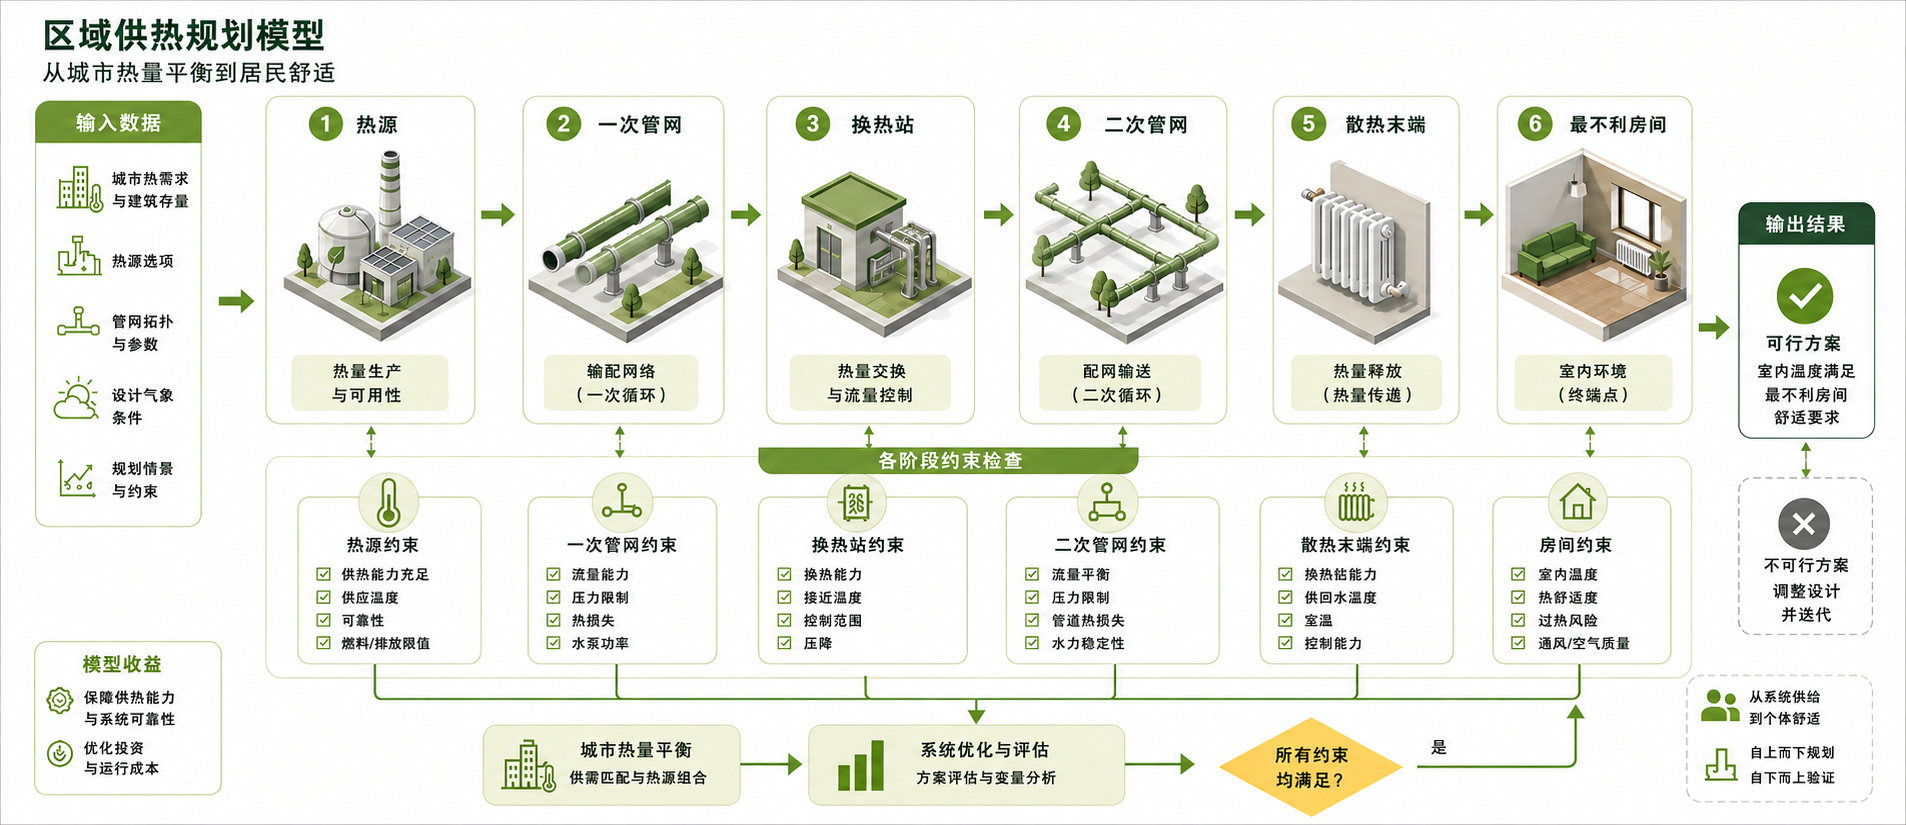
\includegraphics[width=0.714\textwidth,height=0.34\textheight,keepaspectratio]{media/model-figures/128.jpg}
\caption{创新点四：源网荷储与用户侧热惯性协同}
\label{fig:model-128}
\end{figure}

核心创新五：以“优化---压力测试---数值校核”组织求解流程，规划结果进入连续回放与逐时验收。

如图\ref{fig:model-129}所示，该图为优化---校核闭环的\textbf{流程设计}，图中列出温度、水力、回水温度与建筑动态四类校核环节。本次实现的数值校核覆盖节点热平衡、容量、储热状态、配电边界与失供；连续水力、房间级温度与校核结果自动回写作为后续扩展。

\begin{figure}[H]
\centering
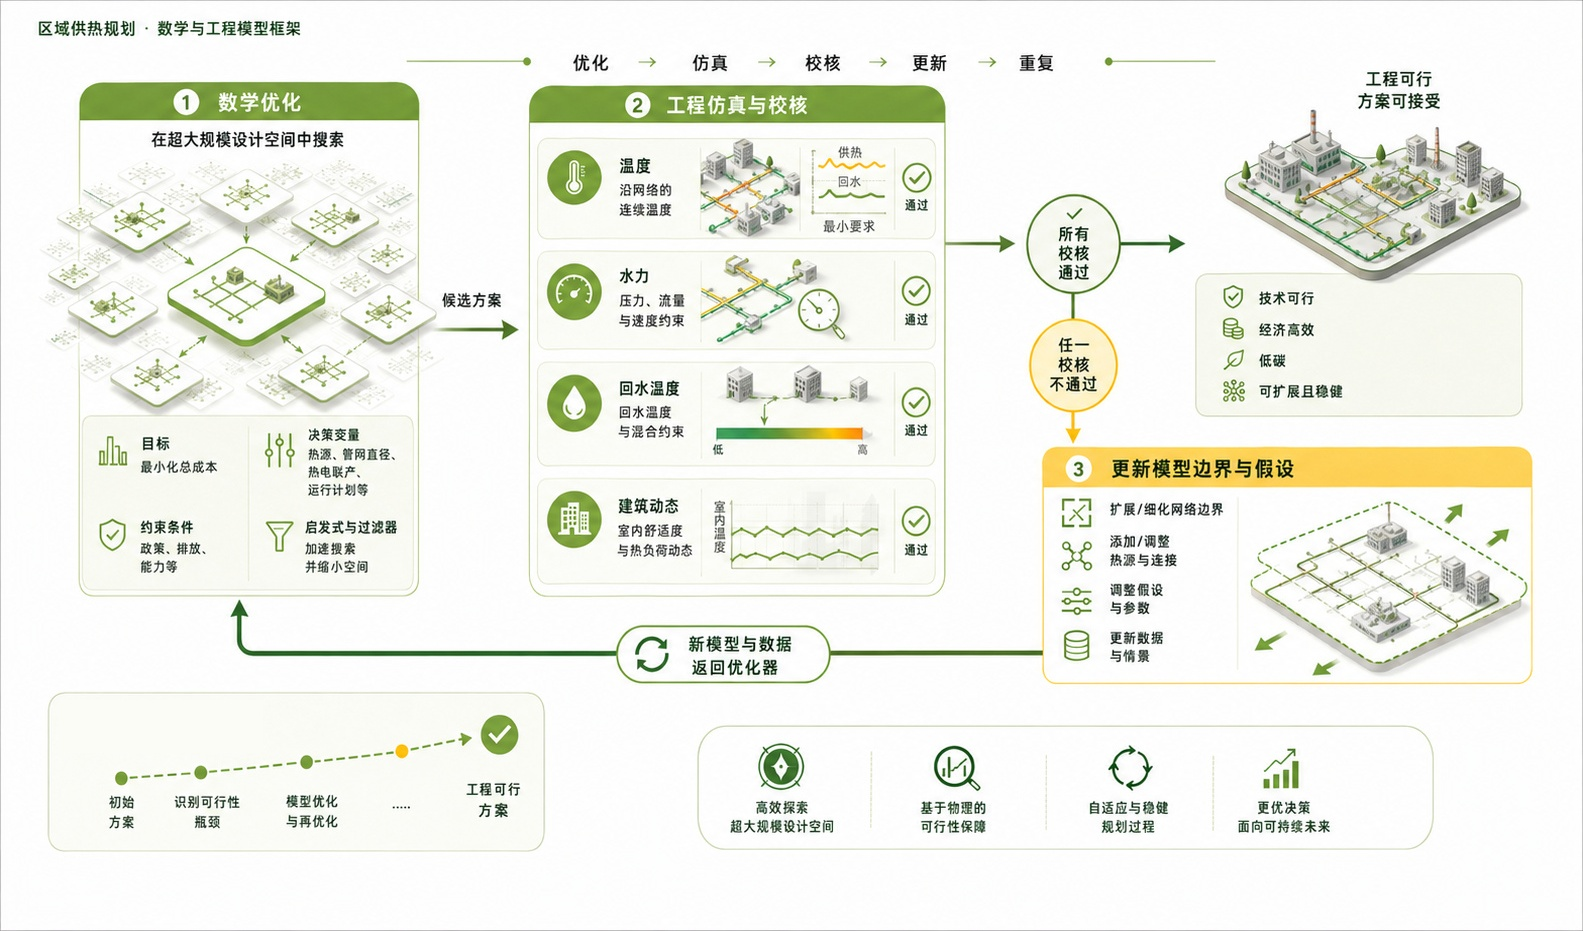
\includegraphics[width=0.714\textwidth,height=0.34\textheight,keepaspectratio]{media/model-figures/129_flow.jpg}
\caption{优化—校核闭环的流程设计}
\label{fig:model-129}
\end{figure}

三个场景采用统一的符号、配置和求解规则完成供暖季计算；连续水力、声学和地源多年动态等专业模块按场景单独复核。

如图\ref{fig:model-130}所示，三个场景共享同一变量集合与物理内核，仅通过配置切换场景专用约束。

\begin{figure}[H]
\centering
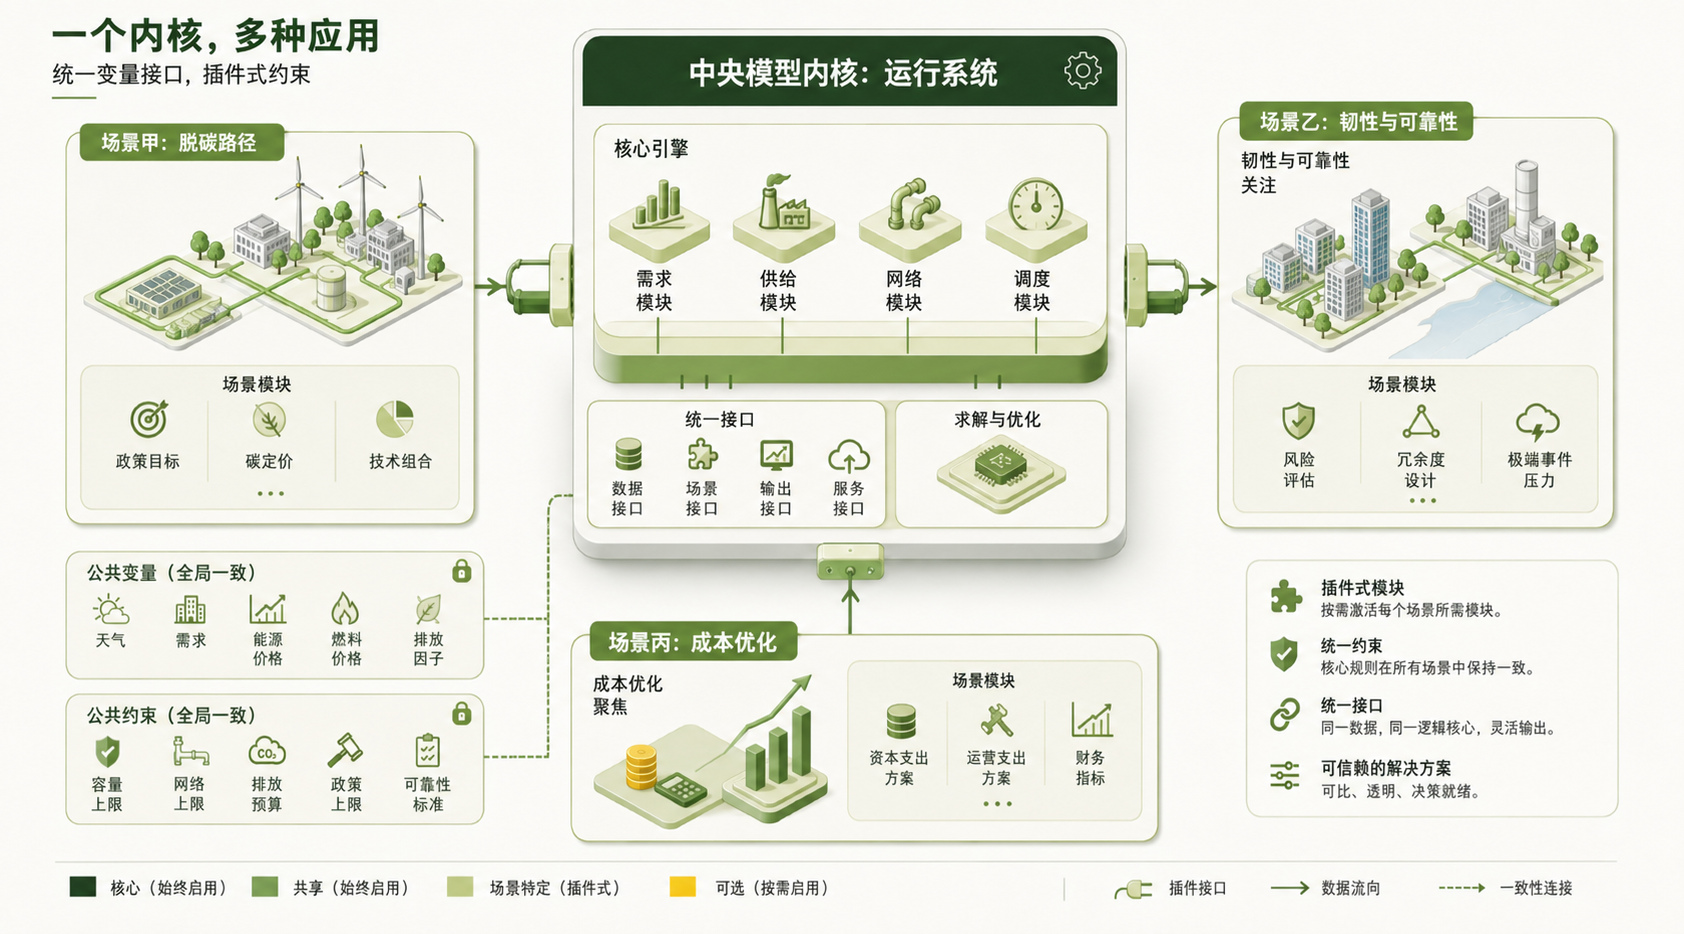
\includegraphics[width=0.714\textwidth,height=0.34\textheight,keepaspectratio]{media/model-figures/130.jpg}
\caption{创新点六：同一内核跨三场景迁移}
\label{fig:model-130}
\end{figure}

\subsection{模型局限}

模型采用固定温位的MILP、有限情景重算和关键断面校核，连续温差---流量、指数温降和非凸水力不直接纳入主模型。建筑热状态采用聚合节点的单一等效热容，未计算房间级温度；热湿、噪声、地源多年动态等模块未在本次算例中启用。模型结果用于规划比较，不能替代施工图、设备选型、地质勘察、环保审批和配电潮流校核。

\enlargethispage{2\baselineskip}
\subsection{结论}

本文将三类供热转型问题统一表述为多年度资产演化、空间组织、带温位多能流、聚合建筑热状态与储能协同优化。三个场景共享公用内核，并分别加载既有热网改造、分散设施选址和夏热冬冷地区供热形态约束。

三个场景采用同一条求解管线：先在代表时段上完成投资---运行联合规划，再冻结投资方案进行完整时序运行校核。本次补充验证在来源锁定的公开输入上重跑了三个场景的全年连续回放，规划层与回放层均取得状态 0 解、失供率为 0，并分别通过 15、16、17 项验收。

本文的一项可迁移经验是：代表时段的锚点覆盖决定了两阶段方法的有效性边界，而锚点规则必须覆盖每一个会绑定约束的极值工况，而不只是负荷峰值。三个场景中只有武汉带供冷服务，旧锚点规则只覆盖集中供热负荷列，全年供冷峰值日因此落在代表时段之外，规划据此定出的冻结容量在全年时序下差 89.6~kW，回放不可行。补齐供冷峰值、采暖最大爬坡与除霜最不利三个锚点后重新规划，供冷可靠性、构模前可靠容量与代表时段覆盖三项验收同时通过。该修正属于涉及结果的实质修订，新旧容量与逐项记录已在同包交付的《仿真结果数据表》中分列登记。

消融与压力测试的既有数值列为历史报告值，连续水力、房间级温度、热湿与噪声等模块列为工程扩展，均不列入本次结果结论。

\clearpage
\begin{center}{\heiti\sihao 参考文献}\end{center}
\addcontentsline{toc}{section}{参考文献}
\begin{refsectionflush}
\refentry{1}{中国建筑科学研究院有限公司.
面向供热格局变革的城镇供热源荷匹配与规划寻优模型构建比赛方案{[}R{]}.
2026.}
\refentry{2}{江亿, 付林, 夏建军, 谢晓云, 吴彦廷, 胡姗.
构建新型零碳热力系统{[}J{]}. 中国工程科学, 2025, 27(5): 1--18. DOI:
10.15302/J-SSCAE-2025.08.025.}
\refentry{3}{Lin Q, Lu S, Yue L, Li B, Zhu H. Research on low-carbon district
heating system planning approach based on thermal energy grade and
integrated demand response{[}EB/OL{]}. SSRN preprint 5082363,
2024/2025（未同行评审预印本）.}
\refentry{4}{Ceruti A, Lambert J, Spliethoff H. Integrating renewable energy
and thermal storage in district heating networks: A design optimization
approach{[}J{]}. Energy Conversion and Management, 2025, 345: 120323.
DOI: 10.1016/j.enconman.2025.120323.}
\refentry{5}{Chen J, Lv H, Ding L, et al.~Multi-objective optimization for
the operation of district heating systems considering flexibility and
economy{[}J{]}. Applied Thermal Engineering, 2025, 263: 125395. DOI:
10.1016/j.applthermaleng.2024.125395.}
\refentry{6}{Lyu Z, Huang M, Liu B, Liu Y. Robust optimization of regional
integrated energy systems considering thermal comfort and uncertainty in
heat networks{[}J{]}. Applied Thermal Engineering, 2025, 275: 126895.
DOI: 10.1016/j.applthermaleng.2025.126895.}
\refentry{7}{崔梦颖, 殷勇高, 赵栋霖, 黄钰希, 曹博文.
地埋管跨季节储热耦合热泵供暖系统性能与经济性分析{[}J{]}. 储能科学与技术,
2026, 15(3): 983--992. DOI: 10.19799/j.cnki.2095-4239.2026.0107.}
\refentry{8}{崔杨, 姜涛, 仲悟之, 崔成伟, 赵钰婷.
考虑风电消纳的区域综合能源系统源荷协调经济调度{[}J{]}. 电网技术, 2020,
44(7): 2474--2482. DOI: 10.13335/j.1000-3673.pst.2019.2317.}
\refentry{9}{李仲博.
基于数字孪生的城镇供热系统按需精准调控技术研究与应用{[}D{]}. 杭州:
浙江大学, 2023.}
\refentry{10}{Paule D, Pakere I, Pubule J, Blumberga D. Optimising
multi-energy community hubs for decarbonisation and energy system
flexibility{[}J{]}. Smart Energy, 2025, 20: 100214. DOI:
10.1016/j.segy.2025.100214.}
\refentry{11}{Zhang Y, Campana P E, Yang Y, et al.~Energy flexibility from
the consumer: Integrating local electricity and heat supplies in a
building{[}EB/OL{]}.}
\refentry{12}{Lu H, Khanna N, Feng W, et al.~China's Electrification
Pathways: Findings from the China Energy Outlook 2022{[}R{]}. Lawrence
Berkeley National Laboratory, 2022.}
\refentry{13}{赵丽丽. 东北农村冬季清洁供暖技术节能改造应用技术研究{[}J{]}.
节能, 2025, 44(11): 88--91. DOI: 10.3969/j.issn.1004-7948.2025.11.018.}
\refentry{14}{白孝轩, 谈润芃, 李朋, 等.
民用燃煤碳排放特征及电能替代减排路径优化{[}J/OL{]}. 环境科学研究, 2026.
DOI: 10.13198/j.issn.1001-6929.2026.06.17.}
\refentry{15}{Wang S, Su H, Chen C, et al.~Natural gas shortages during the
``coal-to-gas'' transition in China have caused a large redistribution
of air pollution{[}EB/OL{]}. arXiv:2004.09585, 2020.}
\refentry{16}{Wang X, Xia L, Bales C, et al.~A systematic review of recent
air source heat pump systems assisted by solar thermal, photovoltaic and
photovoltaic/thermal sources{[}EB/OL{]}. arXiv:2102.09797, 2021.}
\refentry{17}{Xiong C, Hassan M S. Renewable heat policy in China:
Development, achievement, and effectiveness{[}J{]}. Sustainability,
2022, 14: 9297. DOI: 10.3390/su14159297.}
\refentry{18}{Fiorentini M, Baldini L. Control-oriented modelling and
operational optimization of a borehole thermal energy storage{[}J{]}.
Applied Thermal Engineering, 2021: 117518. DOI:
10.1016/j.applthermaleng.2021.117518.}
\refentry{19}{Takam P H, Wunderlich R. Model order reduction for the
input--output behavior of a geothermal energy storage{[}J{]}. Journal of
Engineering Mathematics, 2024, 148: 12. DOI: 10.1007/s10665-024-10398-4.}
\refentry{20}{Li H, Svendsen S. Energy and exergy analysis of low temperature
district heating network{[}J{]}. Energy, 2012, 45(1): 237--246. DOI:
10.1016/j.energy.2012.03.056.}
\refentry{21}{Lund H, Werner S, Wiltshire R, et al.~4th Generation District
Heating (4GDH): Integrating smart thermal grids into future sustainable
energy systems{[}J{]}. Energy, 2014, 68: 1--11. DOI:
10.1016/j.energy.2014.02.089.}
\refentry{22}{Capone M, Guelpa E, Verda V. Potential for supply temperature
reduction of existing district heating substations{[}J{]}. Energy, 2023,
285: 128597. DOI: 10.1016/j.energy.2023.128597.}
\refentry{23}{IPCC. 2006 IPCC Guidelines for National Greenhouse Gas
Inventories, Volume 2: Energy{[}R{]}. Hayama: IGES, 2006.}
\refentry{24}{国务院办公厅. 国务院办公厅关于转发国家发展改革委、住房城乡建设部《加快推动建筑领域节能降碳工作方案》的通知{[}EB/OL{]}. https://www.mee.gov.cn/zcwj/gwywj/202403/t20240318\_1068599.shtml, 访问时间（2026年7月17日）.}
\refentry{25}{国家发展和改革委员会. 加强建筑全过程节能降碳管理，推动建筑领域绿色低碳发展{[}EB/OL{]}. https://www.ndrc.gov.cn/xxgk/jd/jd/202403/t20240321\_1365112.html, 访问时间（2026年7月17日）.}
\refentry{26}{International Energy Agency. Renewable heat: Renewables 2025{[}EB/OL{]}. https://www.iea.org/reports/renewables-2025/renewable-heat, 访问时间（2026年7月17日）.}
\refentry{27}{European Commission. Heating and cooling{[}EB/OL{]}. https://energy.ec.europa.eu/topics/energy-efficiency/heating-and-cooling\_en, 访问时间（2026年7月17日）.}
\end{refsectionflush}



\clearpage
\section*{附录1\quad 场景约束与校核式}
\addcontentsline{toc}{section}{\texorpdfstring{附录1\quad 场景约束与校核式}{附录1 场景约束与校核式}}

\subsection*{A\quad 乌鲁木齐场景}
\addcontentsline{toc}{subsection}{A 乌鲁木齐场景}

\subsubsection*{A.1\quad 热源退役与替代}

燃煤热源退役量不得超过上一阶段已投运容量；达到政策退役年限后，对应容量固定为零：
\begin{equation}
K_{\mathrm{coal},y}^{\mathrm{ret}}\leq K_{\mathrm{coal},y-1}^{\mathrm{exist}},
\qquad y\geq y^{\mathrm{deadline}}\Rightarrow K_{\mathrm{coal},y}^{\mathrm{exist}}=0.
\end{equation}
退役容量由清洁热源、储热有效容量和备用容量共同替代：
\begin{equation}
K_{\mathrm{coal},y}^{\mathrm{ret}}\leq
K_y^{\mathrm{clean,new}}+K_y^{\mathrm{storage,credit}}+K_y^{\mathrm{reserve}}.
\end{equation}
其中，$K_y^{\mathrm{storage,credit}}$表示设计峰值时段可持续提供的放热功率，不等同于储热装置的额定储能量。

\subsubsection*{A.2\quad 余热与热泵}

工业余热利用量受资源供给与回收效率限制：
\begin{equation}
0\leq Q_t^{\mathrm{waste}}\leq\eta^{\mathrm{recovery}}Q_t^{\mathrm{available}}.
\end{equation}

当直接换热设备与余热源热泵取自同一股余热时，分别按设备限出力仍可能重复占用上游热量，因此另设资源池约束。对资源池$r$，直接换热设备集合$\mathcal D_r$与热泵集合$\mathcal H_r$的上游取热合计不得超过资源侧可用热功率：
\begin{equation}
R_{r,t}^{\mathrm{use}}
=\frac{1}{\eta_r^{\mathrm{tr}}}\left[
\sum_{k\in\mathcal D_r}Q_{k,t}
+\sum_{k\in\mathcal H_r}\left(1-\frac{1}{COP_{k,t}}\right)Q_{k,t}
\right]\leq\overline R_{r,t}.
\label{eq:waste-pool}
\end{equation}
其中$\eta_r^{\mathrm{tr}}\in(0,1]$为资源端至设备端的传热效率，热泵的压缩机电力不占余热额度，$\overline R_{r,t}$须由该资源的可用热功率逐时给出。该池按温位共用同一额度，不按温位分别重置。

热泵的热量转换、出力和配电边界为
\begin{align}
Q_t^{\mathrm{HP}}&=COP_tP_t^{\mathrm{HP}},\\
0\leq Q_t^{\mathrm{HP}}&\leq\overline Q^{\mathrm{HP}}u_t^{\mathrm{HP}},\\
P_t^{\mathrm{HP}}+P_t^{\mathrm{base}}+P_t^{\mathrm{pump}}&\leq\overline P^{\mathrm{grid}}.
\end{align}
$COP_t$随热源侧温度、用户侧供水温度和部分负荷率变化。以余热为源的机组，其源侧温位不单独计入火用失配惩罚，源温通过$COP_t$进入模型。

该资源池模块独立于设备容量约束，按声明的资源可用量逐时启用；式\eqref{eq:waste-pool}中的$\overline R_{r,t}$须由资源侧可用热功率给出。本稿三个主算例的配置中，两条余热路径按各自上限取用，资源侧可用热功率的逐时记录尚未取得，现有输入只提供无量纲的可用率序列。这一差别对结论的影响可以直接量化：本次补充验证以无共同预算解的上游取热峰值$1081.53$~kW为基准做单因素额度扫描，逐档登记可行值、对偶界、相对间隙、终止状态与验收结果，详见同包交付的《仿真结果数据表》。额度收到 85\% 及以下各档时，收紧档的对偶界已高于无约束档的可行值，费用上升在 $+0.44\%$ 至 $+3.08\%$ 的区间内可被证明；峰值 100\% 档的费用差 42.65 元小于基准回放自身的相对间隙，属不可分辨的变化。碳排放则不单调，在峰值档附近上升、中段下降、最紧档回升，说明资源侧可用热量是推荐结构的有效约束条件；一旦低于该峰值，方案需要重新规划才能在费用与排放之间重新权衡，本册只登记冻结投资下的运行响应。最紧的 55\% 档在 1800~s 回放时限内未取得最优性证明，其验收未通过，数值只作为该档区间的上端使用。该扫描中的额度是研究设计参数，不是已核验的城市资源量。

\subsubsection*{A.3\quad 温位与水力}

热源$k$与温位$g$的兼容参数定义为
\begin{equation}
A_{kg}^{\mathrm{grade}}=
\begin{cases}
1,&T_k^{\mathrm{src,min}}\geq T_g^{\mathrm{sup}}+\Delta T^{\mathrm{hx}},\\
0,&\text{其他情况}.
\end{cases}
\end{equation}
直接供热量满足$0\leq Q_{k,g,t}^{\mathrm{direct}}\leq A_{kg}^{\mathrm{grade}}\overline Q_k$。关键管段的最大流量利用率为
\begin{equation}
\lambda_e^{\mathrm{flow}}=
\frac{\max_t|\dot m_{e,t}^{\mathrm{exist}}+\dot m_{e,t}^{\mathrm{new}}|}{\overline{\dot m}_e}\leq1.
\end{equation}
管段出口温度采用连续温降模型校核：
\begin{equation}
T_{e,t}^{\mathrm{out}}=T_{e,t}^{\mathrm{env}}+
(T_{e,t}^{\mathrm{in}}-T_{e,t}^{\mathrm{env}})
\exp\left(-\frac{U_eL_e}{\dot m_{e,t}c_p}\right).
\end{equation}
最远换热站的温度裕度满足
\begin{equation}
\Delta T_{n^{\mathrm{far}}}^{\mathrm{margin}}=
\min_t\left(T_{n^{\mathrm{far}},t}^{\mathrm{sup}}-T_{n^{\mathrm{far}},t}^{\mathrm{req}}-\Delta T^{\mathrm{hx}}\right)\geq0.
\end{equation}

\subsubsection*{A.4\quad 回水与可靠性}

换热站供热量、回水温度和最低温差满足
\begin{equation}
Q_{n,t}=\dot m_{n,t}c_p(T_{n,t}^{\mathrm{sup}}-T_{n,t}^{\mathrm{ret}}),
\quad T_{n,t}^{\mathrm{ret}}\leq\overline T_n^{\mathrm{ret}},
\quad T_{n,t}^{\mathrm{sup}}-T_{n,t}^{\mathrm{ret}}\geq\underline{\Delta T}_n.
\end{equation}
关键热源$k$退出时，剩余热源与储热逐时承担负荷：
\begin{equation}
\sum_{j\neq k}Q_{j,t}^{\mathrm{avail}}+Q_t^{\mathrm{storage,dis}}\geq D_t.
\end{equation}
寒潮场景同步修正室外温度、负荷和余热可用量，并要求各时段失供量为零：
\begin{align}
T_t^{\mathrm{out,cold}}&=T_t^{\mathrm{out}}-\Delta T^{\mathrm{cold}},
&D_t^{\mathrm{cold}}&=\alpha_DD_t,\\
Q_t^{\mathrm{waste,cold}}&=\alpha_WQ_t^{\mathrm{waste}},
&Q_t^{\mathrm{un,cold}}&=0.
\end{align}

\subsubsection*{A.5\quad 末端改造}

建筑末端改造变量$z_b^{\mathrm{retro}}\in\{0,1\}$决定最低供水温度：
\begin{equation}
T_b^{\mathrm{req}}=(1-z_b^{\mathrm{retro}})T_b^{\mathrm{old}}+z_b^{\mathrm{retro}}T_b^{\mathrm{new}}.
\end{equation}
管网降温方案同时满足$T_{b,t}^{\mathrm{sup}}\geq T_b^{\mathrm{req}}+\Delta T_b^{\mathrm{hx}}$、改造预算约束和室内最低温度约束。

\subsection*{B\quad 固原场景}
\addcontentsline{toc}{subsection}{B 固原场景}

\subsubsection*{B.1\quad 选址与连通}

候选热源建设、用户分配、服务半径和容量满足
\begin{align}
z_i^{\mathrm{site}}&\in\{0,1\},\qquad
\sum_i x_{i,b}=1,\qquad x_{i,b}\leq z_i^{\mathrm{site}},\\
d_{i,b}x_{i,b}&\leq\overline d_i,\qquad
\sum_bD_b^{\mathrm{peak}}x_{i,b}\leq K_i.
\end{align}
候选管段状态限制热流，热源与用户之间必须存在有效路径：
\begin{equation}
|F_{e,t}|\leq\overline F_ez_e^{\mathrm{pipe}},
\qquad x_{i,b}\leq z_e^{\mathrm{pipe}},
\quad \forall e\in\mathcal P_{i,b}.
\end{equation}
逐段约束保证被分配用户对应路径上的每一条候选管段均已建设；节点热平衡进一步保证路径上的能流连续。

\subsubsection*{B.2\quad 燃料库存}

生物质供热、到货与库存按同一时间轴计算：
\begin{align}
Q_{i,t}^{\mathrm{bio}}\Delta t&=\eta_i^{\mathrm{bio}}H_i^{\mathrm{LHV}}B_{i,t}^{\mathrm{use}},\\
I_{i,t}&=I_{i,t-1}+B_{i,t}^{\mathrm{arrive}}-B_{i,t}^{\mathrm{use}},\\
0\leq I_{i,t}&\leq\overline I_i,\qquad
0\leq B_{i,t}^{\mathrm{arrive}}\leq\overline B_i^{\mathrm{arrive}}.
\end{align}
库存不足时，锅炉出力同步受限：
\begin{equation}
Q_{i,t}^{\mathrm{bio}}\Delta t\leq\eta_i^{\mathrm{bio}}H_i^{\mathrm{LHV}}
(I_{i,t-1}+B_{i,t}^{\mathrm{arrive}}).
\end{equation}
其中$Q^{\mathrm{bio}}$以kW计，$H^{\mathrm{LHV}}$以kWh/kg计，$B^{\mathrm{use}}$以kg计，$\Delta t$以h计。

\subsubsection*{B.3\quad 微网与孤岛}

微网电力平衡及配电容量约束为
\begin{multline}
P_{i,t}^{\mathrm{imp}}+P_{i,t}^{\mathrm{PV}}+P_{i,t}^{\mathrm{bat,dis}}
=P_{i,t}^{\mathrm{base}}+P_{i,t}^{\mathrm{HP}}+P_{i,t}^{\mathrm{EB}}
+P_{i,t}^{\mathrm{pump}}+P_{i,t}^{\mathrm{bat,ch}},\\
P_{i,t}^{\mathrm{imp}}\leq\overline P_i^{\mathrm{grid}}.
\end{multline}
外部电网或单一热源故障时，可用热源与储热满足关键用户负荷：
\begin{equation}
\sum_{k\in\mathcal K_i^{\mathrm{available}}}Q_{k,t}
+Q_{i,t}^{\mathrm{storage,dis}}\geq D_{i,t}^{\mathrm{critical}}.
\end{equation}
完全孤岛状态下，本地电源还应覆盖热泵、电锅炉和循环泵的基本用电。

\subsubsection*{B.4\quad 防冻结与可负担性}

低温运行满足
\begin{equation}
\dot m_{e,t}\geq\dot m_e^{\min},\qquad
T_{e,t}^{\mathrm{ret}}\geq T_e^{\mathrm{freeze}}.
\end{equation}
同时约束运维距离$d_i^{\mathrm{maint}}\leq\overline d_i^{\mathrm{maint}}$和居民供热费用$C_b^{\mathrm{heat}}\leq\overline C_b^{\mathrm{afford}}$。

\subsection*{C\quad 武汉场景}
\addcontentsline{toc}{subsection}{C 武汉场景}

\subsubsection*{C.1\quad 系统形态与多类负荷}

每个区域选择一种基本供热形态：
\begin{equation}
z_i^{\mathrm{building}}+z_i^{\mathrm{station}}+z_i^{\mathrm{LTN}}+z_i^{\mathrm{5GDHC}}=1.
\end{equation}
供热与生活热水平衡、供冷转换和总用电分别为
\begin{align}
Q_{i,t}^{\mathrm{source}}+Q_{i,t}^{\mathrm{storage,dis}}
&=D_{i,t}^{\mathrm{heat}}+D_{i,t}^{\mathrm{DHW}}+Q_{i,t}^{\mathrm{storage,ch}},\\
Q_{i,t}^{\mathrm{cool}}&=COP_{i,t}^{\mathrm{cool}}P_{i,t}^{\mathrm{cool}},\\
P_{i,t}^{\mathrm{total}}&=P_{i,t}^{\mathrm{base}}+P_{i,t}^{\mathrm{heat}}
+P_{i,t}^{\mathrm{cool}}+P_{i,t}^{\mathrm{DHW}}+P_{i,t}^{\mathrm{pump}}.
\end{align}

\subsubsection*{C.2\quad 间歇运行与舒适度}

启动变量和最小连续运行时间满足
\begin{equation}
u_{b,t}-u_{b,t-1}\leq v_{b,t}^{\mathrm{start}},\qquad
\sum_{\tau=t}^{t+T_b^{\min}-1}u_{b,\tau}\geq T_b^{\min}v_{b,t}^{\mathrm{start}}.
\end{equation}
供暖期和供冷期分别设置室温范围，相对湿度和最低新风量满足
\begin{equation}
RH_b^{\min}\leq RH_{b,t}\leq RH_b^{\max},\qquad
V_{b,t}^{\mathrm{vent}}\geq\underline V_b^{\mathrm{vent}}.
\end{equation}

\subsubsection*{C.3\quad 结露与除霜}

室内表面和低温管网均应高于露点并保留安全裕度：
\begin{equation}
T_{b,t}^{\mathrm{surface}}\geq T_{b,t}^{\mathrm{dew}}+\Delta T^{\mathrm{safe}},
\qquad T_{e,t}^{\mathrm{sup}}\geq T_{e,t}^{\mathrm{dew}}+\Delta T_e^{\mathrm{safe}}.
\end{equation}
空气源热泵除霜期间的实际供热量和耗电量为
\begin{equation}
Q_t^{\mathrm{HP,actual}}=(1-\phi_t^{\mathrm{defrost}})Q_t^{\mathrm{HP,rated}},
\qquad P_t^{\mathrm{HP,actual}}=P_t^{\mathrm{HP,rated}}+P_t^{\mathrm{defrost}}.
\end{equation}

\subsubsection*{C.4\quad 地源、噪声与配电}

地源系统年度取热与排热比值约束为
\begin{equation}
r^{\min}\sum_tQ_t^{\mathrm{inj}}\Delta t
\leq\sum_tQ_t^{\mathrm{ext}}\Delta t
\leq r^{\max}\sum_tQ_t^{\mathrm{inj}}\Delta t.
\end{equation}
其中$Q^{\mathrm{ext}}$为从地下取热功率，$Q^{\mathrm{inj}}$为向地下排热功率，$\Delta t$为时间步长。该式属于可选约束，本次三个算例均未启用。
正常时段和夜间分别设置噪声上限。楼栋配电容量满足
\begin{equation}
P_{b,t}^{\mathrm{HP}}+P_{b,t}^{\mathrm{cool}}+P_{b,t}^{\mathrm{DHW}}+P_{b,t}^{\mathrm{base}}
\leq P_b^{\mathrm{exist}}+K_b^{\mathrm{grid,new}}.
\end{equation}

\subsection*{D\quad 统一校核}
\addcontentsline{toc}{subsection}{D 统一校核}

三类场景均检查以下基础条件：
\begin{align}
\max_t|r_t^{\mathrm{heat}}|&\leq\varepsilon_Q,&
\max_t|r_t^{\mathrm{storage}}|&\leq\varepsilon_E,\\
\theta_b^{\min}\leq\theta_{b,t}^{a}&\leq\theta_b^{\max},&
\lambda_e^{\mathrm{flow}}&\leq1,\\
P_{n,t}^{\mathrm{imp}}&\leq\overline P_n^{\mathrm{grid}},&
U^{\mathrm{un}}&=0.
\end{align}
乌鲁木齐增加资产退役、温位匹配、管网降温与寒潮保供校核；固原增加热源选址、微网连通、燃料库存、孤岛运行和防冻结校核；武汉增加冷热水耦合、热湿舒适、结露、除霜、地源平衡、噪声和楼栋配电校核。


\section*{附录2\quad 符号与缩略语说明}
\addcontentsline{toc}{section}{\texorpdfstring{附录2\quad 符号与缩略语说明}{附录2 符号与缩略语说明}}

本文仅列出模型中频繁使用的典型符号。程序输入与逐时调度采用kW、kWh和kg，汇总表可换算为MW、MWh和t；换算关系分别为$1~\mathrm{MW}=10^3~\mathrm{kW}$、$1~\mathrm{MWh}=10^3~\mathrm{kWh}$和$1~\mathrm{t}=10^3~\mathrm{kg}$。摄氏温差与开尔文温差数值相同；涉及火用计算时，绝对温度由$T(\mathrm K)=\theta({}^{\circ}\mathrm C)+273.15$换算。

\begin{table}[H]
\centering
\caption{典型符号说明}
\begin{tabular}{p{0.16\textwidth}p{0.43\textwidth}p{0.28\textwidth}}
\toprule
符号 & 含义 & 单位\\
\midrule
$c$ & 供热转型场景编号（C1、C2、C3） & --\\
$y$ & 规划阶段或年份 & --\\
$t$ & 运行时段 & h\\
$\omega$ & 不确定情景 & --\\
$n$ & 网络节点或建筑节点 & --\\
$k$ & 设备类型 & --\\
$x$ & 第一阶段规划决策变量 & --\\
$q_\omega$ & 情景$\omega$下运行变量 & --\\
$K$ & 设备容量变量 & kW（汇总时可换算为MW）\\
$SOC$ & 储能状态变量 & kWh（汇总时可换算为MWh）\\
$C$ & 聚合节点等效热容 & kWh/K\\
$R$ & 等效热阻 & K/kW\\
$\theta$ & 室温或等效温度偏移 & $^{\circ}$C\\
$H$ & 围护与通风合并的总传热系数 & kW/K\\
$\lambda$ & 逐时恢复损失率或储热自损失率 & $\mathrm h^{-1}$\\
$Q$ & 热功率 & kW\\
$D$ & 热需求 & kW\\
$u$ & 设备启停状态 & --\\
$C_{net}$ & 生命周期净成本 & 元\\
$EENS$ & 期望失供能量 & MWh\\
$COP$ & 热泵性能系数 & --\\
\bottomrule
\end{tabular}
\end{table}

常用缩略语包括：MILP（混合整数线性规划）、CHP（热电联产）、TES（储热系统）、BTES（跨季节地埋管储热）、CVaR（条件风险价值）、EENS（期望失供能量）。

\clearpage
\section*{附录3\quad 三场景推荐配置模板}\label{ux9644ux5f55-a-ux4e09ux573aux666fux63a8ux8350ux914dux7f6eux6a21ux677f}
\addcontentsline{toc}{section}{\texorpdfstring{附录3\quad 三场景推荐配置模板}{附录3 三场景推荐配置模板}}

\begin{Verbatim}[breaklines=true,breakanywhere=true,fontsize=\small]
common:
  objective: deterministic_lifecycle_cost
  time_structure: [chronological_typical_periods, extreme_design_day]
  uncertainty: post_optimization_scenarios_and_sensitivity
  validation: [key_section_hydraulics, terminal_and_return_temperature, selected_full_chronology]
scenario_C1:
  full_numerical_case: true
  modules: [temperature_grade_matching, three_state_network, endogenous_retirement, short_term_storage, building_terminal_and_deltaT]
scenario_C2:
  full_numerical_case: true
  modules: [facility_siting, user_assignment, microgrid_topology, distributed_heat_pump, biomass_logistics]
scenario_C3:
  full_numerical_case: true
  modules: [system_form_selection, heating_cooling_DHW, thermal_comfort, defrosting, grid_peak]
advanced_optional:
  modules: [C_and_CG, logic_Benders, automatic_engineering_cuts, full_BTES_multiyear, online_MPC]
\end{Verbatim}

附录配置只定义模块开关和数据字段，不提供全国默认参数。实际配置位于交付包的三场景配置目录，供暖季输入与逐时输出按场景分别存放；参数来源、年份、单位、适用区域和不确定区间应在项目数据字典中逐项记录。运行前先按\texttt{README.md}核对解释器、依赖、配置路径和输入文件，再用验收记录检查已有结果。

本次补充验证的完整实验登记（三场景输入与配置、逐方案求解与连续验收、共享容量单因素对照、工业余热共同预算扫描、代表时段锚点修正）按赛题“仿真结果数据表”一栏单独成册，与本报告同包交付，正文不再重复列出。
\end{document}
